\documentclass[a4paper,12pt]{report}
% \usepackage[table]{xcolor}
\usepackage[utf8]{inputenc}
\usepackage[T1]{fontenc}
\usepackage[portuguese]{babel}
\usepackage{hyperref}
\usepackage{tikz}
\usepackage{emoji}
\usetikzlibrary{arrows.meta, positioning, shapes}
\usepackage{amsmath}
\usepackage{tabularx} % Inclua isso no preâmbulo do seu documento
\usepackage{makecell}
\usepackage{array}
\usepackage{graphicx}
\usepackage{float}
\usepackage{multirow}
\usetikzlibrary{shapes.geometric, arrows, shadows, trees}
\tikzstyle{segment} = [rectangle, rounded corners, text centered, draw=black, fill=green!30]
\tikzstyle{arrow} = [thick,->,>=stealth]
\usepackage{pgfplots}
\usepackage{emoji}
\usepackage{makecell}

\begin{document}

\title{\textbf{Classificação de Descrições de Produtos em Português: Avaliação de Técnicas de Recuperação da Informação e o Impacto de seus Parâmetros}}
\author{Gilsiley Henrique Darú}

\date{\today}
\maketitle

\chapter*{Resumo}

	A crescente demanda por classificação de informações baseada em conteúdo na era das mídias sociais e do comércio eletrônico tem levado à necessidade de classificação automatizada de produtos com base nas suas descrições. Este estudo tem como objetivo avaliar várias técnicas para essa tarefa, com ênfase em descrições escritas em português. Uma pipeline é implementada para pré-processar os dados, incluindo conversão para minúsculas, remoção de acentos e separação por espaço de unigramas. Em seguida, o método sacola de palavras é usado para converter o texto em dados numéricos e cinco técnicas de classificação são aplicadas: argmaxtf, argmaxtfnorm, argmaxtfidf proveniente da recuperação de informação.           
				\vspace{0.15cm}
        \noindent \textbf{Palavras-chave:} aprendizado de máquina; processamento de linguagem natural; classificação de texto; descrição do produto; texto curto; sacola de palavras; frequencia de termos; frequencia inversa de documentos

	
     
% Adicione o resumo aqui.

\tableofcontents

% Conteúdo da introdução.
\chapter{Introdução}

\section{Contextualização do Problema}


% Na era atual de digitalização massiva, onde mais de 2.5 quintilhões de bytes \cite{gandomi2015137} são gerados diariamente, o crescimento acelerado de redes sociais e plataformas de e-commerce intensificou a demanda por métodos eficientes de classificação de textos. Essa necessidade não se restringe apenas à otimização da experiência do usuário, mas se estende a várias aplicações, incluindo filtragem de spam, análise de sentimento e personalização de publicidade \cite{alsmadi2019review}.

Na era atual de digitalização massiva, onde mais de 2.5 quintilhões de bytes \cite{gandomi2015137} são gerados diariamente, o crescimento acelerado de redes sociais e plataformas de e-commerce intensificou a demanda por métodos eficientes de classificação de textos. Esse vasto volume de dados exige sistemas automatizados que possam organizar e categorizar informações de maneira rápida e precisa, para otimizar a experiência do usuário e facilitar diversas aplicações, como filtragem de spam, análise de sentimento e personalização de publicidade \cite{alsmadi2019review}.


No contexto do idioma português, com suas particularidades, regionalismos e nuances entre variantes como o português do Brasil e de Portugal, a classificação textual apresenta desafios adicionais\cite{branco2012lingua}. Inclua-se o objetivo do trabalho, utilização de textos curtos, descrição curta é definida como um texto com até 200 caracteres, o que acrescenta uma camada de complexidade à tarefa, dado o conteúdo limitado disponível para análise \cite{alsmadi2019review} e \cite{song2014short}.

\subsection*{Exemplo do Problema de Categorização de Texto em Português}

Para ilustrar os desafios da categorização de textos curtos em português, considere a tarefa de identificar produtos da categoria "BISCOITO" em uma lista. A busca direta pela palavra "biscoito" retornaria resultados como "BISCOITO DUX SALGADO 648G" e "BISCOITO CRACKERS DUX 216G". No entanto, muitas descrições utilizam abreviações como "BISC LEITE MABEL 400G" e "BISC.PARATI MARIA PE 370GR", que seriam ignoradas pela busca simples.

Além disso, termos regionais ou estrangeiros como "BOLACHA", "COOKIE" e "COOKIES" também devem ser considerados, por exemplo, "BOLACHA PAPAGUARA MOTOR 400g" e "COOKIES GRAN CASTANH PARA KOBBER 150G". A complexidade aumenta quando produtos não relacionados são incluídos na busca, como "BISC PET CRACKER FORTAL 400G" (biscoitos para animais de estimação) e "CESTA SUPREME BISCOITO LIMAO 100G" (cesta de presentes), ou itens como camisetas com estampas que mencionam "BISCOITO".

\begin{figure}[h!]
    \begin{center}
    \caption{Camiseta com a palavra BISCOITO estampada}
    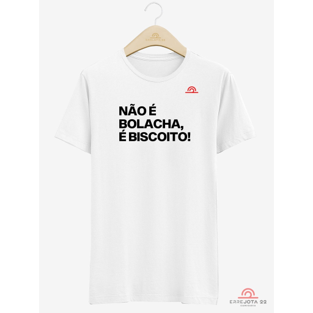
\includegraphics[scale=0.5]{images/camiseta.png}
    \label{fig:camiseta}
    \end{center}
\end{figure}

Esses exemplos demonstram a necessidade de métodos mais avançados para garantir uma classificação precisa.


% Suponha que se faz necessário encontrar, a partir de uma lista, todos os produtos que são da categoria "BISCOITO".  A primeira ideia é buscar por uma única palavra, por exemplo "biscoito".  Utilizando-se esta ideia encontra-se descrições como "BISCOITO DUX SALGADO 648G" e "BISCOITO CRACKERS DUX 216G".

% No entanto, há outras descrições de produtos onde "BISCOITO" é abreviado como "BISC LEITE MABEL 400G" e "BISC.PARATI MARIA PE 370GR", e esses resultados não seriam mostrados. Devido a este problema de abreviação e com o objetivo de realizar esta tarefa usando uma lista de palavras, seria necessário expandir a lista de palavras de busca para abranger as novas palavras "BISC" e "BISC." para serem reconhecidas como "BISCOITO".

% Também existem outras palavras completamente diferentes que deveriam retornar como resultado da busca por "BISCOITO". Essas palavras são, às vezes, termos locais ou estrangeiros e, novamente, precisaríamos expandir a lista de vocabulário. Por exemplo, "BOLACHA PAPAGUARA MOTOR 400g", "COOKIE INT BAUDUCCO AVEIA PASSAS 40G" e "COOKIES GRAN CASTANH PARA KOBBER 150G" onde as novas palavras são "BOLACHA", "COOKIE" e "COOKIES".

% Mesmo assim, essa solução aditiva não resolve completamente o problema, pois há algumas descrições contendo a palavra "BISCOITO", mas de fato não são. Por exemplo, "BISC PET CRACKER FORTAL 400G" e "BISC PET DOG CROCK 500G" são biscoitos para animais de estimação e "BISC LACTA BIS FLOWP 126G, LAKA BCO" e "CESTA SUPREME BISCOITO LIMAO 100G" são, respectivamente, chocolate e cesta de presentes. E uma camiseta estampada "NÃO É BOLACHA, É BISCOITO!" mostrada na Figura \ref{fig:camiseta} da mesma forma seria retornada pela pesquisa mas que não pertence a categoria desejada.

% \begin{figure}[h!]
%     \begin{center}
%     \caption{Camiseta com a palavra BISCOITO estampada}
%     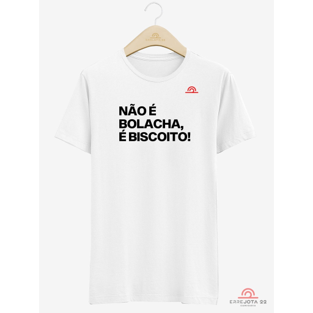
\includegraphics[scale=0.5]{images/camiseta.png}
%     \label{fig:camiseta}
%     \end{center}
%      %\small\textbf{Fonte:} Os autores.
% \end{figure}

% \section{Hipóteses}


% Diversas pesquisas têm indicado a variabilidade no desempenho dos algoritmos de aprendizado de máquina dependendo da técnica e do dataset em questão \cite{alsmadi2019review} e \cite{aggarwal2018review}. Técnicas de pré-processamento, como remoção de stopwords, stemming e lematização, podem ter um impacto significativo no desempenho dos modelos \cite{naseem2021survey}. Outro ponto a se considerar são os hiperparâmetros de cada modelo e sua otimização, que provocam significativas alterações nas medidas de avaliação de desempenho \cite{bhavani2021review}.

% \textbf{Hipótese:} Algoritmos de aprendizado de máquina, quando combinados com técnicas adequadas de pré-processamento e otimização de hiperparâmetros, podem melhorar significativamente a precisão, acurácia, recall e F1-score na classificação de descrições curtas de produtos em português.

\section{Hipóteses}

Diversas pesquisas têm indicado a variabilidade no desempenho dos algoritmos de recuperação da informação dependendo da técnica e do dataset em questão \cite{alsmadi2019review} e \cite{aggarwal2018review}. Técnicas de pré-processamento, como remoção de stopwords, stemming e lematização, podem ter um impacto significativo no desempenho dos modelos \cite{naseem2021survey}. Outro ponto a se considerar são os parâmetros de cada modelo e sua otimização, que provocam significativas alterações nas medidas de avaliação de desempenho \cite{bhavani2021review}.

\textbf{Hipótese:} Algoritmos simples de recuperação da informação, quando combinados com técnicas adequadas de pré-processamento e otimização de parâmetros, podem melhorar significativamente a precisão, acurácia, recall e F1-score na classificação de descrições curtas de produtos em português.



% Diversas pesquisas têm indicado a variabilidade no desempenho dos algoritmos de aprendizado de máquina dependendo da técnica e do dataset em questão \cite{alsmadi2019review} e \cite{aggarwal2018review}. Técnicas de pré-processamento, como remoção de stopwords, stemming e lematização, podem ter um impacto significativo no desempenho dos modelos\cite{naseem2021survey}. Outro ponto a se considerar são os hiperparâmetros de cada modelo e sua otimização provocam significativas alteração nas medidas de avaliação de desempenho \cite{bhavani2021review}.

% \section{Objetivos Gerais}

% O objetivo central deste estudo é analisar o desempenho, medido em termos de acurácia, precisão, recall e F1-score, de diferentes algoritmos de aprendizado de máquina na classificação de descrições curtas de produtos em português, utilizando o dataset DARU como referência.

% \subsection{Objetivos Específicos}

% Dentro deste escopo, busca-se:

% \begin{enumerate}
%     \item Avaliar o desempenho de algoritmos tradicionais e modernos, incluindo SVMs, regressão logística e redes neurais, na classificação de textos curtos.
%     \item Analisar o impacto de diferentes técnicas de pré-processamento, como remoção de stopwords, stemming e lematização, na eficácia dos modelos.
%     \item Determinar e otimizar os hiperparâmetros mais adequados para cada algoritmo.
% \end{enumerate}

\section{Objetivos Gerais}

O objetivo central deste estudo é analisar o desempenho, medido em termos de acurácia e F1-score macro, de diferentes algoritmos de recuperação da informação adaptados para a classificação de descrições curtas de produtos em português, utilizando o dataset DARU como referência.

\subsection{Objetivos Específicos}

Dentro deste escopo, busca-se:

\begin{enumerenumerate}
    \item Adaptar métodos de recuperação da informação, como sacola de palavras, TF e TF-IDF, para servirem como classificadores de descrições curtas de produtos.
    \item Avaliar o desempenho de algoritmos simples de recuperação da informação, como TF e TF-IDF com métricas de similaridade, na classificação de textos curtos em português.
    \item Analisar o impacto de diferentes técnicas de pré-processamento, como normalização e diferentes abordagens de tokenização, na eficácia dos modelos de recuperação da informação.
    \item Determinar e otimizar os parâmetros mais adequados para cada algoritmo, visando maximizar a acurácia e o F1-score macro.
    \item Adaptar uma métrica que unifique a acurácia e o F1-score macro para a avaliação de desempenho.
\end{enumerenumerate}

% \section{Justificativa e Relevância}

% A classificação apropriada de descrições de produtos é importante para a experiência do usuário, empresas e profissionais de e-commerce. Esta pesquisa, ao avaliar diferentes técnicas, oferece resultados consistentes para a área de processamento de linguagem natural e aprendizado de máquina, servindo como guia inicial para implementações mais eficazes.

\section{Justificativa e Relevância}

A classificação apropriada de descrições de produtos é relevante para a experiência do usuário, empresas e profissionais de e-commerce. Para os usuários, uma classificação eficiente facilita a busca por produtos, melhora a navegabilidade e personaliza as recomendações. Para as empresas, um sistema de classificação robusto otimiza a organização do catálogo de produtos, melhora a precisão das campanhas de marketing e aumenta a eficiência operacional.



% No contexto do idioma português, com suas particularidades, regionalismos e variações, a tarefa de classificação de textos curtos torna-se ainda mais desafiadora. Este estudo, ao adaptar e avaliar diferentes técnicas de recuperação da informação, oferece soluções práticas e aplicáveis para o mercado brasileiro, contribuindo para a melhoria das ferramentas de e-commerce e processamento de linguagem natural.


% \section{Metodologia}

% Nesta pesquisa, é adotada uma abordagem quantitativa para investigar o desempenho dos algoritmos de aprendizado de máquina na classificação de descrições curtas de produtos em português. O dataset DARU é utilizado como material principal, devido à sua relevância e abrangência no contexto brasileiro.

% A garantia da integridade e qualidade dos dados é obtida através da \textbf{Preparação dos Dados}. Esta etapa engloba o pré-processamento dos dados, no qual é feita a limpeza para remover qualquer inconsistência ou ruído, é realizada a remoção de stopwords - palavras comuns que podem não agregar valor significativo ao texto, e são aplicadas técnicas como stemming e lematização, que respectivamente reduzem as palavras à sua raiz e transformam palavras em sua forma base. Essa fase é essencial para assegurar que os algoritmos operem eficientemente e produzam resultados consistentes.

% Após a preparação, é realizada a \textbf{Seleção de Modelos}. Nesta etapa, são explorados diferentes algoritmos de aprendizado de máquina, desde abordagens tradicionais, como Máquinas de Vetores de Suporte (SVM) e regressão logística, até métodos mais contemporâneos como redes neurais. A escolha desses modelos é baseada em sua popularidade, eficácia comprovada e relevância para a tarefa de classificação de textos.

% Com os modelos selecionados, é feito o \textbf{Treinamento e Teste}. Os algoritmos escolhidos são treinados utilizando uma porção do dataset DARU. Para evitar o sobreajuste e garantir que os modelos tenham uma boa generalização, é empregada a técnica de validação cruzada estratificada. Esta abordagem envolve a divisão do dataset em múltiplos subconjuntos de forma que cada subconjunto seja usado tanto para treinamento quanto para teste, garantindo que todas as classes sejam representadas proporcionalmente.

% Finalmente, após o treinamento e teste dos modelos, é realizada a \textbf{Avaliação}. Nessa fase, o desempenho dos modelos é avaliado com base em métricas padrão, como acurácia, precisão, recall e F1-score. Estas métricas ajudam a entender o desempenho dos algoritmos, permitindo identificar os mais adequados para a tarefa em questão e fornecer insights sobre possíveis ajustes e otimizações.


\section{Metodologia}

Nesta pesquisa, é adotada uma abordagem quantitativa para investigar o desempenho dos algoritmos de recuperação da informação na classificação de descrições curtas de produtos em português. O dataset DARU é utilizado como material principal, devido à sua relevância e abrangência no contexto brasileiro.

\subsection{Preparação dos Dados}
A garantia da integridade e qualidade dos dados é obtida através do pré-processamento dos dados. Esta etapa inclui a limpeza para remover inconsistências ou ruído, normalização para padronizar os textos, e a aplicação de diferentes abordagens de tokenização. Essas técnicas asseguram que os algoritmos operem eficientemente e produzam resultados consistentes.

\subsection{Seleção e Adaptação de Algoritmos}
Nesta etapa, são adaptados diferentes métodos de recuperação da informação, como sacola de palavras, TF e TF-IDF, para servirem como classificadores. A adaptação envolve agrupar as descrições em um documento, onde cada documento representa uma categoria, e a aplicação de métricas de similaridade para determinar a categoria mais provável de cada descrição de produto.

\subsection{Treinamento e Teste}
Os algoritmos escolhidos são treinados utilizando uma porção do dataset DARU. Para evitar o sobreajuste e garantir uma boa generalização, é empregada a técnica de validação cruzada estratificada. Esta abordagem envolve a divisão do dataset em múltiplos subconjuntos, garantindo que todas as classes sejam representadas proporcionalmente.

\subsection{Avaliação}
O desempenho dos modelos é avaliado com base em métricas padrão, como acurácia e F1-score macro. Estas métricas ajudam a entender o desempenho dos algoritmos, permitindo identificar os mais adequados para a tarefa em questão e fornecer insights sobre possíveis ajustes e otimizações.

\subsection{Proposta de Métrica Unificada}
Além das métricas padrão, é proposto a adaptação de uma métrica que unifique a acurácia e o F1-score macro para a avaliação de desempenho dos algoritmos de recuperação da informação.

% \section{Contribuições}

% As principais contribuições deste trabalho são:

% \begin{itemize}
%     \item Uma análise aprofundada do desempenho de diferentes algoritmos de aprendizado de máquina na classificação de textos curtos em português.
%     \item Diretrizes sobre as técnicas de pré-processamento mais eficazes para esta tarefa.
%     \item Recomendações para otimização de hiperparâmetros para diferentes algoritmos.
% \end{itemize}

\section{Contribuições}

As principais contribuições deste trabalho são:

\begin{itemize}
    \item Uma análise aprofundada do desempenho de diferentes algoritmos de recuperação da informação na classificação de textos curtos em português.
    \item Diretrizes sobre as técnicas de pré-processamento mais eficazes para esta tarefa.
    \item Recomendações para otimização de parâmetros para diferentes algoritmos de recuperação da informação.
    \item Adaptação de uma métrica unificada que combina acurácia e F1-score macro.
\end{itemize}


% \section{Estrutura do Trabalho}

% Este trabalho é estruturado da seguinte forma:

% \begin{enumerate}
%     \item \textbf{Introdução:} Contextualização do problema, objetivos, justificativa e relevância.
%     \item \textbf{Revisão Literária:} Discussão sobre trabalhos anteriores, técnicas e algoritmos relevantes.
%     \item \textbf{Metodologia:} Descrição detalhada da abordagem adotada na pesquisa.
%     \item \textbf{Resultados:} Apresentação e discussão dos resultados obtidos.
%     \item \textbf{Conclusão:} Resumo dos achados, contribuições e sugestões para trabalhos futuros.
% \end{enumerate}

\section{Estrutura do Trabalho}

Este trabalho é estruturado da seguinte forma:

\begin{enumerate}
    \item \textbf{Introdução:} Contextualização do problema, objetivos, justificativa e relevância.
    \item \textbf{Revisão Literária:} Discussão sobre trabalhos anteriores, técnicas e algoritmos relevantes.
    \item \textbf{Metodologia:} Descrição detalhada da abordagem adotada na pesquisa, incluindo a adaptação de algoritmos de recuperação da informação.
    \item \textbf{Resultados:} Apresentação e discussão dos resultados obtidos.
    \item \textbf{Conclusão:} Resumo dos achados, contribuições e sugestões para trabalhos futuros.
\end{enumerate}



% \section{CIMO - Contexto, Problema, Objetivo, Método e Contribuição}

% \subsection{Contexto}
% Na era atual de digitalização massiva, a classificação textual tornou-se uma ferramenta essencial, especialmente no domínio do e-commerce e redes sociais. Com a crescente quantidade de dados gerados diariamente, métodos eficazes de categorização são cruciais.

% \subsection{Problema}
% Dada a rica complexidade do idioma português e a necessidade de classificar textos curtos, como descrições de produtos, existe uma demanda por algoritmos de aprendizado de máquina eficientes e precisos para esta tarefa.

% \subsection{Objetivo}
% O estudo visa analisar e otimizar o desempenho de diferentes algoritmos de aprendizado de máquina na classificação de descrições curtas de produtos em português.

% \subsection{Método}
% Serão utilizados diversos algoritmos, desde abordagens tradicionais até técnicas mais modernas, avaliando o impacto de diferentes técnicas de pré-processamento e otimização de hiperparâmetros.

% \subsection{Contribuição}
% Esta pesquisa espera contribuir para a área de processamento de linguagem natural e aprendizado de máquina, fornecendo diretrizes e práticas recomendadas para a classificação de textos curtos em português.

\section{CIMO - Contexto, Problema, Objetivo, Método e Contribuição}

\subsection{Contexto}
Na era atual de digitalização massiva, a classificação textual tornou-se uma ferramenta essencial, especialmente no domínio do e-commerce e redes sociais. Com a crescente quantidade de dados gerados diariamente, métodos eficazes de categorização são necessários.

\subsection{Problema}
Dada a complexidade do idioma português e a necessidade de classificar textos curtos, como descrições de produtos, existe uma demanda por algoritmos de recuperação da informação eficientes e precisos para esta tarefa.

\subsection{Objetivo}
O estudo visa analisar e otimizar o desempenho de diferentes algoritmos de recuperação da informação na classificação de descrições curtas de produtos em português.

\subsection{Método}
Serão utilizados diversos algoritmos de recuperação da informação, como sacola de palavras, TF e TF-IDF, avaliando o impacto de diferentes técnicas de pré-processamento e otimização de parâmetros.

\subsection{Contribuição}
Esta pesquisa espera contribuir para a área de processamento de linguagem natural, fornecendo diretrizes e práticas recomendadas para a classificação de textos curtos em português, além de adaptar uma métrica unificada que combina acurácia e F1-score macro.


\chapter{Revisão Sistemática}

\section{Introdução}

Esta revisão sistemática tem como objetivo identificar e analisar os estudos mais relevantes sobre técnicas de classificação de textos curtos, com um foco particular em descrições de produtos em português. A pesquisa é conduzida nas bases Scopus e Web of Science, utilizando os termos de pesquisa ("text* classification*" OR "text* categori\$ation*" OR "document* classification*" OR "document* categori\$ation*") como primeiro tema e ("machine learning" OR "machine* learn*" OR "ML" OR "artificial intelligence" OR "AI") como segundo tema. Os critérios de inclusão limitaram os resultados ao idioma Inglês e Português, com buscas realizadas nos títulos, resumos e palavras-chave, e restringindo-se a artigos de jornais e conferências.

\section{Métodos}

A pesquisa de literatura foi conduzida nas bases Scopus e Web of Science, utilizando os seguintes termos de pesquisa: "text* classification*" OR "text* categori\$ation*" OR "document* classification*" OR "document* categori\$ation*" e "machine learning" OR "machine* learn*" OR "ML" OR "artificial intelligence" OR "AI". A busca foi limitada aos idiomas Inglês e Português, abrangendo títulos, resumos e palavras-chave. Apenas artigos de jornais e conferências foram incluídos. Os critérios de inclusão foram: relevância para a classificação de textos curtos, enfoque em técnicas de aprendizado de máquina ou recuperação da informação, e pertinência ao contexto do idioma português. Artigos duplicados, revisões, e publicações sem acesso ao texto completo foram excluídos.

\section{Evolução das Palavras Chaves}

As análises destacadas são evolução das palavras chaves, principais jornais e conferências da área, artigos mais citados e evolução da quantidade de publicações no tempo.

A quantidade de artigos encontrados foi de 7169, tendo o assunto de classificação de texto um crescimento de 8,49\% ao ano.  A Figura \ref{fig:historicotexto} apresenta um pico em 2021 e um leve decrescimento para 2021, mas já apresentando artigos para o tema para o ano de 2023. Verifica-se um rápido crescimento nos últimos anos no tema, isto é justificado pelo fato da tarefa estar diretamente aplicada a função de organização da informação.  

\begin{figure}[htb]
    \caption{Evolução Histórica dos artigos sobre classificação de texto nos últimos anos}
    \begin{center}    
    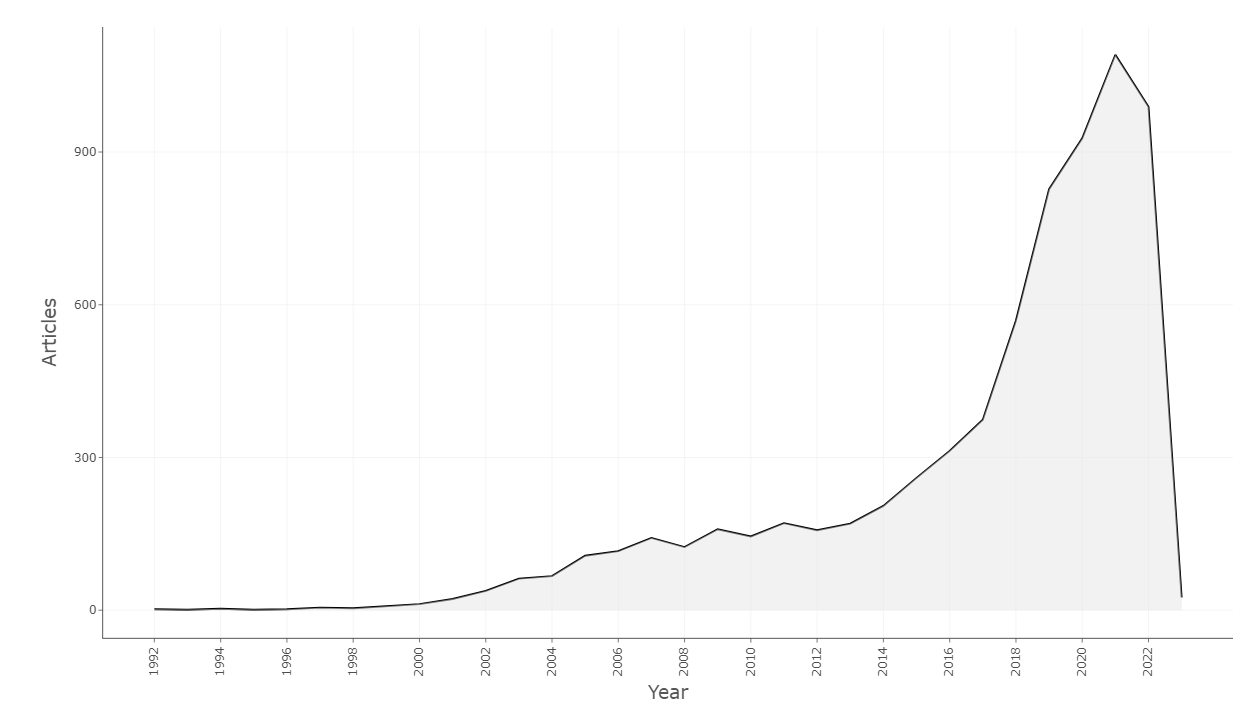
\includegraphics[scale=0.3]{images/evolucaoclassificacao.png}
    \label{fig:historicotexto}
    \end{center}
     \small\textbf{Origem:}  O autor.
\end{figure}

\section{Principais Jornais e Conferências}

Com relação a jornais e conferências, a Tabela \ref{tab:origem-acumulado} mostra que não há uma concentração significativa de publicações. As dez principais fontes representam 12,2\% do total de publicações, o que demonstra uma ampla aplicabilidade do tema. É importante mencionar o primeiro jornal, que é um periódico de acesso aberto na Europa. Os próximos dois são repositórios tradicionais de artigos científicos nas áreas: ACM e IEEE. Outro jornal a se destacar é "Expert Systems With Applications". Além disso, vale mencionar que existem mais de 3600 fontes e mais de 14.000 autores envolvidos na amostra coletada.

\begin{table}[h]
\centering
\begin{tabular}{ >{\raggedright\arraybackslash}m{5cm} | >{\raggedleft\arraybackslash}m{1.5cm} | >{\raggedleft\arraybackslash}m{1.5cm} | >{\raggedleft\arraybackslash}m{1.5cm} }
\hline
\textbf{Origem} & \textbf{Quant.} & \textbf{Total} & \textbf{\%} \\ \hline
\makecell[{{p{5cm}}}]{CEUR Workshop Proceedings} & 228 & 228 & 3,2 \\ \hline
\makecell[{{p{5cm}}}]{ACM International Conference Proceeding Series} & 143 & 371 & 5,2 \\ \hline
IEEE Access & 133 & 504 & 7,0 \\ \hline
\makecell[{{p{5cm}}}]{Expert Systems with Applications} & 68 & 572 & 8,0 \\ \hline
Journal of Biomedical Informatics & 60 & 632 & 8,8 \\ \hline
Applied Sciences-Basel & 52 & 684 & 9,5 \\ \hline
\makecell[{{p{5cm}}}]{Journal of Physics: Conference Series} & 52 & 736 & 10,3 \\ \hline
Neurocomputing & 49 & 785 & 10,9 \\ \hline
\makecell[{{p{5cm}}}]{IJCAI International Joint Conference on Artificial Intelligence} & 48 & 833 & 11,6 \\ \hline
\makecell[{{p{5cm}}}]{International Journal of Advanced Computer Science and Applications} & 41 & 874 & 12,2 \\ \hline
\end{tabular}
\caption{Principais fontes de publicações sobre classificação de textos, quantidade de artigos por fonte, total acumulado e porcentagem do total de publicações.}
\label{tab:origem-acumulado}
\end{table}

\section{Artigos Mais Citados}

A Tabela \ref{tab:autores-titulos} apresenta uma lista de artigos de referência na área de classificação de texto, ordenados por número de citações. Destacam-se os trabalhos que tratam de técnicas de pré-processamento e modelos de aprendizado de máquina relevantes para a classificação de descrições de produtos, como técnicas para evitar super ajuste do aprendizado \cite{srivastava2014dropout}, aprendizado de transferência \cite{pan2010survey}, e métricas de desempenho \cite{sokolova2009systematic}.

\begin{table}[h]
\centering
\begin{tabular}{ >{\raggedright\arraybackslash}m{8cm} | >{\raggedleft\arraybackslash}m{2.5cm} | >{\raggedleft\arraybackslash}m{1.5cm} }
\hline
\textbf{Título} & \textbf{Citações} & \textbf{Ano} \\ \hline
\cite{srivastava2014dropout} & 19002 & 2014 \\ \hline
\cite{pan2010transfer} & 9633 & 2010 \\ \hline
\cite{sebastiani2002machine} & 3854 & 2002 \\ \hline
\cite{sokolova2009systematic} & 2472 & 2009 \\ \hline
\cite{zhang2007mlknn} & 1852 & 2007 \\ \hline
\cite{forman2003extensive} & 1843 & 2003 \\ \hline
\cite{le2014distributed} & 1772 & 2014 \\ \hline
\cite{quoc2014distributed} & 1663 & 2014 \\ \hline
\cite{dave2003mining} & 1483 & 2003 \\ \hline
\cite{tong2002support} & 1445 & 2002 \\ \hline
\cite{joachims2006training} & 1417 & 2006 \\ \hline
\cite{lai2015recurrent} & 1251 & 2015 \\ \hline
\cite{kusner2015word} & 1133 & 2015 \\ \hline
\cite{howard2018universal} & 1116 & 2018 \\ \hline
\cite{raffel2020exploring} & 1056 & 2020 \\ \hline
\cite{raina2007self} & 998 & 2007 \\ \hline
\cite{bottou2018optimization} & 876 & 2018 \\ \hline
\cite{tschantaridis2004support} & 841 & 2004 \\ \hline
\cite{natekin2013gradient} & 821 & 2013 \\ \hline
\cite{rennie2003tackling} & 760 & 2003 \\ \hline
\end{tabular}
\caption{Artigos mais citados na área de classificação de textos, incluindo número de citações e ano de publicação.}
\label{tab:autores-titulos}
\end{table}

\section{Discussão}

A classificação de textos curtos concentra-se em textos com até 200 caracteres, sendo comum em aplicações como análise de sentimentos em redes sociais e classificação de opiniões em resenhas de produtos. Devido ao comprimento limitado, técnicas de pré-processamento e extração de características são fundamentais para capturar as informações mais relevantes.

Devido ao comprimento limitado dos textos, as técnicas de classificação de texto curto geralmente se concentram em capturar as características mais relevantes dos textos para a classificação. Isso pode incluir técnicas de pré-processamento para remover stop words e normalizar o texto, bem como técnicas de extração de características para resumir o conteúdo do texto em um conjunto de características relevantes.

Além disso, a classificação de texto curto também pode se beneficiar de técnicas de aprendizado de máquina, como redes neurais, que podem ser treinadas para capturar padrões complexos nos textos curtos. Embora os modelos de linguagem como word2VEC e BERT sejam muito populares para classificação de texto mais longo, também existem modelos de linguagem específicos para classificação de texto curto, como ULMFiT, que foram projetados para lidar com textos curtos.

Em geral, a classificação de texto curto é uma área em constante evolução, e os 153 artigos encontrados demonstram a crescente importância dessa área. A combinação de técnicas de pré-processamento, extração de características e aprendizado de máquina tem permitido o desenvolvimento de modelos cada vez mais precisos e eficientes para classificar textos curtos.

\section{Lacunas na Literatura}

Apesar do avanço significativo nas técnicas de classificação de textos, algumas lacunas foram identificadas na literatura. Há uma carência de estudos focados especificamente na classificação de textos curtos em português, bem como uma falta de comparações sistemáticas entre diferentes abordagens de pré-processamento e algoritmos de classificação. Além disso, poucos estudos exploram o impacto das variações regionais do idioma português na eficácia dos modelos de classificação.

\section{Análise Crítica}

A análise dos estudos revisados revela que as técnicas de aprendizado de máquina, como SVM, Naive Bayes e redes neurais, são amplamente utilizadas para a classificação de textos curtos. No entanto, a eficácia dessas técnicas varia significativamente dependendo das estratégias de pré-processamento adotadas. Estudos que utilizam técnicas avançadas de pré-processamento, como lematização e remoção de stopwords, tendem a apresentar melhores resultados de acurácia e F1-score. Por outro lado, alguns estudos apontam desafios relacionados à sobreajuste e a necessidade de otimização dos hiperparâmetros para cada modelo. A aplicação de modelos de linguagem, como word2VEC e BERT, tem mostrado resultados promissores, mas a adaptação desses modelos para o português ainda é um campo em desenvolvimento.

% \section{Limitações do Estudo}

% Esta revisão sistemática apresenta algumas limitações que devem ser consideradas ao interpretar os resultados. Primeiramente, a pesquisa foi limitada a artigos em inglês e português, o que pode ter excluído estudos relevantes publicados em outros idiomas. Além disso, apenas artigos de jornais e conferências foram incluídos, excluindo teses, dissertações e literatura cinzenta que poderiam conter informações valiosas. Outra limitação é a potencial variabilidade na qualidade dos estudos incluídos, que pode influenciar os resultados e conclusões da revisão. Finalmente, a rápida evolução das técnicas de classificação de textos pode significar que alguns estudos recentes não foram capturados devido ao tempo necessário para a publicação e indexação dos artigos.


% \chapter{Revisão Sistemática}

% \section{Introdução}

% \section{Introdução}

% Esta revisão sistemática tem como objetivo identificar e analisar os estudos mais relevantes sobre técnicas de classificação de textos curtos, com um foco particular em descrições de produtos em português. 


% \section{Métodos}

% A pesquisa de literatura foi conduzida nas bases Scopus e Web of Science, utilizando os seguintes termos de pesquisa: "text* classification*" OR "text* categori\$ation*" OR "document* classification*" OR "document* categori\$ation*" e "machine learning" OR "machine* learn*" OR "ML" OR "artificial intelligence" OR "AI". A busca foi limitada aos idiomas Inglês e Português, abrangendo títulos, resumos e palavras-chave. Apenas artigos de jornais e conferências foram incluídos. Os critérios de inclusão foram: relevância para a classificação de textos curtos, enfoque em técnicas de aprendizado de máquina ou recuperação da informação, e pertinência ao contexto do idioma português. Artigos duplicados, revisões, e publicações sem acesso ao texto completo foram excluídos.


% % Apresenta-se uma pesquisa de literatura sobre as bases Scopus e Web of Science, utilizando-se os termos de pesquisa ( "text* classification*"  OR  "text* categori\$ation*"  OR  "document* classification*"  OR  "document* categori\$ation*" ) como primeiro tema e ("machine learning" OR "machine* learn*" OR "ML" OR "artificial intelligence" OR "AI") como segundo tema.  Foram limitados para o idioma Inglês e Português, busca no título, abstract e palavras chaves e limitando apenas a jornais e conferências.

% \section{Evolução das Palavras Chaves}

% As análises destacadas são evolução das palavras chaves, principais jornais e conferências da área, artigos mais citados e evolução da quantidade de publicações no tempo.

% A quantidade de artigos encontrados foi de 7169, tendo o assunto de classificação de texto um crescimento de 8,49\% ao ano.  A Figura \ref{fig:historicotexto} apresenta um pico em 2021 e um leve decrescimento para 2021, mas já apresentando artigos para o tema para o ano de 2023.  Verifica-se um rápido crescimento nos últimos anos no tema, isto é justificado pelo fato da tarefa estar diretamente aplicada a função de organização da informação.  

% \begin{figure}[htb]
%     \caption{Evolução Histórica dos artigos sobre classificação de texto nos últimos anos}
%     \begin{center}    
%     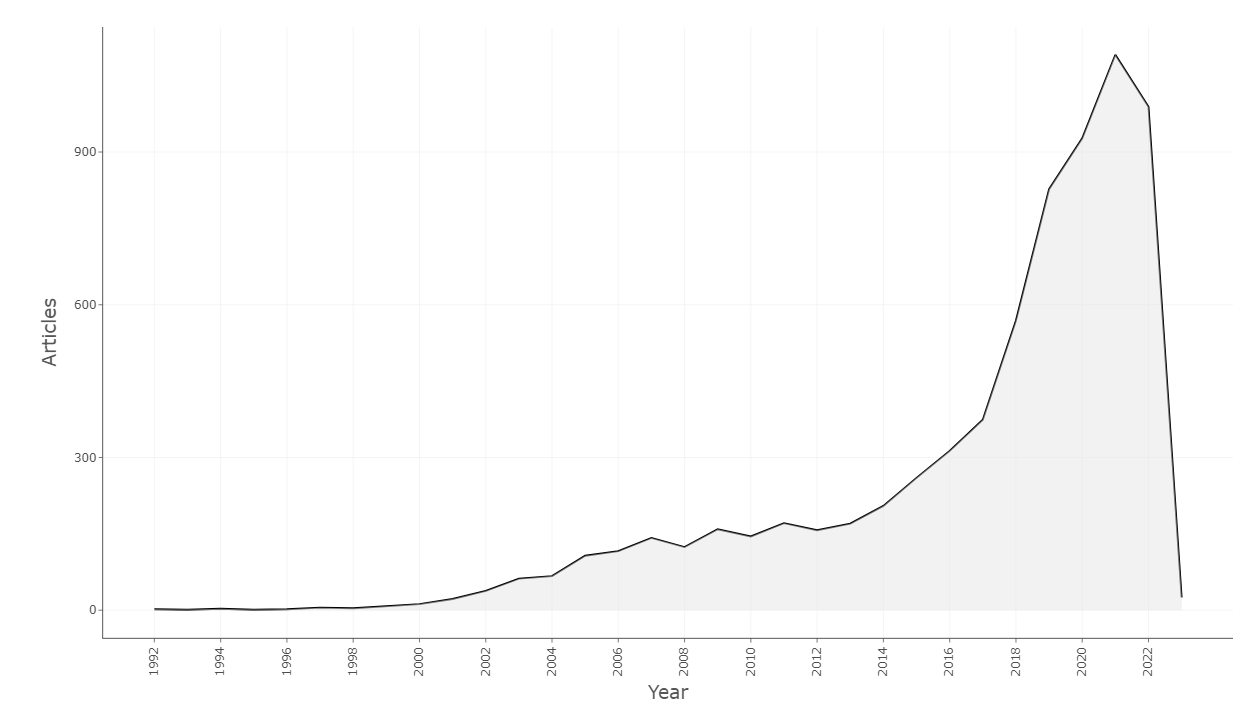
\includegraphics[scale=0.3]{images/evolucaoclassificacao.png}
%     \label{fig:historicotexto}
%     \end{center}
%      \small\textbf{Origem:}  O autor.
% \end{figure}

% \section{Principais Jornais e Conferências}

% Com relação a jornais e conferências, a Tabela \ref{tab:origem-acumulado} mostra que não há uma concentração significativa de publicações. As dez principais fontes representam 12,2\% do total de publicações, o que demonstra uma ampla aplicabilidade do tema. É importante mencionar o primeiro jornal, que é um periódico de acesso aberto na Europa. Os próximos dois são repositórios tradicionais de artigos científicos nas áreas: ACM e IEEE. Outro jornal a se destacar é "Expert Systems With Applications". Além disso, vale mencionar que existem mais de 3600 fontes e mais de 14.000 autores envolvidos na amostra coletada.


% \begin{table}[h]
% \centering
% \begin{tabular}{ >{\raggedright\arraybackslash}m{5cm} | >{\raggedleft\arraybackslash}m{1.5cm} | >{\raggedleft\arraybackslash}m{1.5cm} | >{\raggedleft\arraybackslash}m{1.5cm} }
% \hline
% \textbf{Origem} & \textbf{Quant.} & \textbf{Total} & \textbf{\%} \\ \hline
% \makecell[{{p{5cm}}}]{CEUR Workshop Proceedings} & 228 & 228 & 3,2 \\ \hline
% \makecell[{{p{5cm}}}]{ACM International Conference Proceeding Series} & 143 & 371 & 5,2 \\ \hline
% IEEE Access & 133 & 504 & 7,0 \\ \hline
% \makecell[{{p{5cm}}}]{Expert Systems with Applications} & 68 & 572 & 8,0 \\ \hline
% Journal of Biomedical Informatics & 60 & 632 & 8,8 \\ \hline
% Applied Sciences-Basel & 52 & 684 & 9,5 \\ \hline
% \makecell[{{p{5cm}}}]{Journal of Physics: Conference Series} & 52 & 736 & 10,3 \\ \hline
% Neurocomputing & 49 & 785 & 10,9 \\ \hline
% \makecell[{{p{5cm}}}]{IJCAI International Joint Conference on Artificial Intelligence} & 48 & 833 & 11,6 \\ \hline
% \makecell[{{p{5cm}}}]{International Journal of Advanced Computer Science and Applications} & 41 & 874 & 12,2 \\ \hline
% \end{tabular}
% \caption{Principais fontes de publicações sobre classificação de textos, quantidade de artigos por fonte, total acumulado e porcentagem do total de publicações.}
% \label{tab:origem-acumulado}
% \end{table}



% % A Tabela \ref{tab:autores-titulos} apresenta uma lista de artigos de referência na área de aprendizado de máquina para classificação de texto, ordenados por número de citações. É possível observar que os artigos mais citados tratam de técnicas para evitar super ajuste do aprendizado e como o método "Dropout" proposto pode auxiliar \cite{srivastava2014dropout}, bem como estudos sobre aprendizado de transferência \cite{pan2010survey} e métricas de desempenho para tarefas de classificação \cite{sokolova2009systematic}. Outros tópicos abordados incluem aprendizado passivo \cite{zhang2007mlknn}, seleção de recursos \cite{forman2003extensive}, representações distribuídas de sentenças e documentos \cite{le2014distributed} e modelos de processamento de linguagem natural como o "Universal Language Model Finetuning" \cite{howard2018universal}.
% % É importante notar que esses artigos abrangem muitos anos de publicação, desde 2002 até 2020, e isso demonstra que a área tem-se desenvolvido constantemente e continuará a desenvolver-se no futuro.

% \section{Artigos Mais Citados}

% A Tabela \ref{tab:autores-titulos} apresenta uma lista de artigos de referência na área de classificação de texto, ordenados por número de citações. Destacam-se os trabalhos que tratam de técnicas de pré-processamento e modelos de aprendizado de máquina relevantes para a classificação de descrições de produtos, como técnicas para evitar super ajuste do aprendizado \cite{srivastava2014dropout}, aprendizado de transferência \cite{pan2010survey}, e métricas de desempenho \cite{sokolova2009systematic}.


% \usepackage{makecell}
% \usepackage{array}

% \begin{table}[h]
% \centering
% \begin{tabular}{ >{\raggedright\arraybackslash}m{8cm} | >{\raggedleft\arraybackslash}m{2.5cm} | >{\raggedleft\arraybackslash}m{1.5cm} }
% \hline
% \textbf{Título} & \textbf{Citações} & \textbf{Ano} \\ \hline
% \cite{srivastava2014dropout} & 19002 & 2014 \\ \hline
% \cite{pan2010transfer} & 9633 & 2010 \\ \hline
% \cite{sebastiani2002machine} & 3854 & 2002 \\ \hline
% \cite{sokolova2009systematic} & 2472 & 2009 \\ \hline
% \cite{zhang2007mlknn} & 1852 & 2007 \\ \hline
% \cite{forman2003extensive} & 1843 & 2003 \\ \hline
% \cite{le2014distributed} & 1772 & 2014 \\ \hline
% \cite{quoc2014distributed} & 1663 & 2014 \\ \hline
% \cite{dave2003mining} & 1483 & 2003 \\ \hline
% \cite{tong2002support} & 1445 & 2002 \\ \hline
% \cite{joachims2006training} & 1417 & 2006 \\ \hline
% \cite{lai2015recurrent} & 1251 & 2015 \\ \hline
% \cite{kusner2015word} & 1133 & 2015 \\ \hline
% \cite{howard2018universal} & 1116 & 2018 \\ \hline
% \cite{raffel2020exploring} & 1056 & 2020 \\ \hline
% \cite{raina2007self} & 998 & 2007 \\ \hline
% \cite{bottou2018optimization} & 876 & 2018 \\ \hline
% \cite{tschantaridis2004support} & 841 & 2004 \\ \hline
% \cite{natekin2013gradient} & 821 & 2013 \\ \hline
% \cite{rennie2003tackling} & 760 & 2003 \\ \hline
% \end{tabular}
% \caption{Artigos mais citados na área de classificação de textos, incluindo número de citações e ano de publicação.}
% \label{tab:autores-titulos}
% \end{table}


% A classificação de texto é um tema que tem evoluído ao longo dos anos, e que pode ser dividido em três eixos: preparação da informação, técnicas e aplicações. No que diz respeito à preparação da informação, a evolução do tema começou com técnicas determinísticas, seguidas por técnicas estatísticas e matriciais. Mais recentemente, a aplicação de redes neurais tem permitido o desenvolvimento de modelos de linguagem aprimorados, como word2VEC e BERT.

% No eixo das técnicas, a tendência foi semelhante, iniciando-se com técnicas determinísticas, seguida por técnicas matriciais. No entanto, houve uma grande aplicação de técnicas de aprendizado de máquina, como KNN, Naive Bayes e SVM, seguida por técnicas agregadas, como Ensemble e Boosting. Mais recentemente, tem-se utilizado diversas arquiteturas de redes neurais, como CNN, RNN, modelos de Atenção e Transformers.

% Por fim, no eixo das aplicações, é possível ver a versatilidade da área de classificação de texto. As aplicações estão presentes em campos como a saúde, o direito, a identificação de autoria, a exploração de sentimentos em redes sociais e linguagens específicas, como Chinês e Árabe. Além disso, aplicações como chatbot, sumarização de texto, classificação hierárquica e bulling também são mencionadas. A lista de aplicações levantadas inclui mais de 50 exemplos.

% Em resumo, a classificação de texto é um tema amplo e em constante evolução, que abrange desde a preparação da informação até as técnicas e aplicações mais recentes. A utilização de técnicas estatísticas e matriciais, seguida pela utilização de redes neurais, tem permitido o desenvolvimento de modelos cada vez mais precisos e eficientes. Além disso, as aplicações são amplas e abrangem diferentes campos e linguagens.




% \section{Discussão}

% A classificação de textos curtos concentra-se em textos com até 200 caracteres, sendo comum em aplicações como análise de sentimentos em redes sociais e classificação de opiniões em resenhas de produtos. Devido ao comprimento limitado, técnicas de pré-processamento e extração de características são fundamentais para capturar as informações mais relevantes.

% Devido ao comprimento limitado dos textos, as técnicas de classificação de texto curto geralmente se concentram em capturar as características mais relevantes dos textos para a classificação. Isso pode incluir técnicas de pré-processamento para remover stop words e normalizar o texto, bem como técnicas de extração de características para resumir o conteúdo do texto em um conjunto de características relevantes.

% Além disso, a classificação de texto curto também pode se beneficiar de técnicas de aprendizado de máquina, como redes neurais, que podem ser treinadas para capturar padrões complexos nos textos curtos. Embora os modelos de linguagem como word2VEC e BERT sejam muito populares para classificação de texto mais longo, também existem modelos de linguagem específicos para classificação de texto curto, como ULMFiT, que foram projetados para lidar com textos curtos.

% Em geral, a classificação de texto curto é uma área em constante evolução, e os 153 artigos encontrados demonstram a crescente importância dessa área. A combinação de técnicas de pré-processamento, extração de características e aprendizado de máquina tem permitido o desenvolvimento de modelos cada vez mais precisos e eficientes para classificar textos curtos.

% \section{Lacunas na Literatura}

% Apesar do avanço significativo nas técnicas de classificação de textos, algumas lacunas foram identificadas na literatura. Há uma carência de estudos focados especificamente na classificação de textos curtos em português, bem como uma falta de comparações sistemáticas entre diferentes abordagens de pré-processamento e algoritmos de classificação. Além disso, poucos estudos exploram o impacto das variações regionais do idioma português na eficácia dos modelos de classificação.

% \section{Análise Crítica}

% A análise dos estudos revisados revela que as técnicas de aprendizado de máquina, como SVM, Naive Bayes e redes neurais, são amplamente utilizadas para a classificação de textos curtos. No entanto, a eficácia dessas técnicas varia significativamente dependendo das estratégias de pré-processamento adotadas. Estudos que utilizam técnicas avançadas de pré-processamento, como lematização e remoção de stopwords, tendem a apresentar melhores resultados de acurácia e F1-score. Por outro lado, alguns estudos apontam desafios relacionados à sobreajuste e a necessidade de otimização dos hiperparâmetros para cada modelo. A aplicação de modelos de linguagem, como word2VEC e BERT, tem mostrado resultados promissores, mas a adaptação desses modelos para o português ainda é um campo em desenvolvimento.


% \section{Análise Crítica}

% A classificação de textos curtos concentra-se em textos com até 200 caracteres, sendo comum em aplicações como análise de sentimentos em redes sociais e classificação de opiniões em resenhas de produtos. Devido ao comprimento limitado, técnicas de pré-processamento e extração de características são fundamentais para capturar as informações mais relevantes.



% % Classificação de texto curto é uma área específica da classificação de texto que se concentra em classificar textos com comprimentos curtos, geralmente até 200 caracteres. Esta área é comumente utilizada em aplicações como análise de sentimento em redes sociais, onde os comentários e postagens são curtos, e classificação de opiniões em resenhas de produtos, entre outras.

% Devido ao comprimento limitado dos textos, as técnicas de classificação de texto curto geralmente se concentram em capturar as características mais relevantes dos textos para a classificação. Isso pode incluir técnicas de pré-processamento para remover stop words e normalizar o texto, bem como técnicas de extração de características para resumir o conteúdo do texto em um conjunto de características relevantes.

% Além disso, a classificação de texto curto também pode se beneficiar de técnicas de aprendizado de máquina, como redes neurais, que podem ser treinadas para capturar padrões complexos nos textos curtos. Embora os modelos de linguagem como word2VEC e BERT sejam muito populares para classificação de texto mais longo, também existem modelos de linguagem específicos para classificação de texto curto, como ULMFiT, que foram projetados para lidar com textos curtos.

% Em geral, classificação de texto curto é uma área em constante evolução, e os 153 artigos encontrados demonstram a crescente importância dessa área. A combinação de técnicas de pré-processamento, extração de características e aprendizado de máquina tem permitido o desenvolvimento de modelos cada vez mais precisos e eficientes para classificar textos curtos.


\chapter{Fundamentos}

\section{Introdução}

% Neste capítulo, busca-se apresentar uma revisão abrangente dos conceitos fundamentais e das principais abordagens na literatura relacionada à classificação de textos curtos. A compreensão desses conceitos é importante para contextualizar e fundamentar as discussões e análises nos capítulos subsequentes.

% A organização do capítulo é a seguinte: inicia-se com uma seção sobre os conceitos fundamentais, onde são definidos e explicados os principais conceitos e terminologias relacionados à classificação de textos curtos. Avança-se, então, para a revisão da literatura, abrangendo áreas como a evolução histórica do tema, abordagens convencionais e técnicas de aprendizado de máquina aplicadas à classificação de textos curtos. Será realizada uma análise crítica das técnicas existentes, destacando suas limitações, lacunas e controvérsias na literatura, e a relevância da pesquisa atual em relação aos trabalhos anteriores.

% Ao final do capítulo, conclui-se os principais pontos discutidos, estabelecendo uma base sólida para os capítulos subsequentes. Esta estrutura visa uma compreensão do estado da arte no campo da classificação de textos curtos e a identificação de oportunidades para pesquisa futura e desenvolvimento de novas técnicas.


Neste capítulo, apresenta-se uma revisão dos conceitos básicos e das principais abordagens na literatura relacionada à classificação de textos curtos. Esses conceitos são importantes para contextualizar as discussões e análises nos capítulos subsequentes.

O capítulo está organizado da seguinte forma: inicialmente, são definidos e explicados os conceitos e terminologias principais. Em seguida, realiza-se uma revisão da literatura, cobrindo a evolução histórica do tema, abordagens convencionais e técnicas de aprendizado de máquina aplicadas à classificação de textos curtos. Além disso, é feita uma análise crítica das técnicas existentes, destacando suas limitações e a relevância da pesquisa atual.

Ao final do capítulo, resume-se os principais pontos discutidos, estabelecendo uma base para os capítulos subsequentes. Esta estrutura busca proporcionar uma visão geral do estado da arte na classificação de textos curtos e identificar oportunidades para futuras pesquisas e desenvolvimento de novas técnicas.

\section{Classificação de Texto Curto}

\subsection{Definição}

A Classificação de texto consiste em atribuir uma classe ou categoria pré-definida a um conjunto de texto. É uma tarefa comum em processamento de linguagem natural e é utilizada para organizar, estruturar e categorizar grandes quantidades de dados \cite{kowsari2019text} .

Os algoritmos de classificação de texto recebem como entrada um conjunto de texto e produzem uma classe. A classe é escolhida a partir de um conjunto pré-definido de categorias ou rótulos. 
Formalmente, de acordo com \cite{aggarwal2012survey}, um problema de classificação envolve um conjunto de instâncias $D = {X_1,...,X_n}$, onde cada instância pertence a uma das $k$ classes indexadas por ${1,2,...,k}$. Aqui, $X_i$ é um exemplo, como uma descrição de produto, e $n$ é o número de instâncias. Na Figura \ref{fig:produtos_categorias}, é apresentada a associação entre as descrições dos itens e suas respectivas categorias, onde se observa $n=3$ itens distintos relacionados às suas classes ($k=2$).

\begin{figure}[htbp]
    \centering
\begin{tikzpicture}[
    box/.style={draw, rectangle, minimum width=4cm, minimum height=1cm, anchor=west},
    title/.style={font=\bfseries},
    arrow/.style={->, thick}
]

% Titles
\node[title] (itemdesc) at (0,0) {Itens};
\node[title] (classes) at (6,0) {Classes};

% Left column items
\node[box] (x1) at (0,-1) {$X_1$ bisc recheado};
\node[box] (x2) at (0,-2.5) {$X_2$ refri lar lt 350ml};
\node[box] (x3) at (0,-4) {$X_3$ refri lim g 600};

% Right column categories
\node[box] (c1) at (6,-1) {1.Biscoito};
\node[box] (c2) at (6,-2.5) {2.Refrigerante};

% Arrows
\draw[arrow] (x1.east) -- (c1.west);
\draw[arrow] (x2.east) -- (c2.west);
\draw[arrow] (x3.east) -- (c2.west);

\end{tikzpicture}

\caption{Associação de produtos e suas categorias}
    \label{fig:produtos_categorias}
\end{figure}

Um conjunto de treinamento é usado para construir um modelo de classificação, que é utilizado para prever a classe de uma nova instância desconhecida. Este problema pode ser considerado difícil quando a classe é explicitamente determinada ou suave quando são atribuídas probabilidades. A classificação de texto requer a conversão de texto em dados numéricos, o que pode ser alcançado por meio de técnicas de processamento de linguagem natural, mostrados em seção posterior.

\subsubsection{Texto Curto}

Texto curto é definido, extraído de \cite{alsmadi2019review} como um texto de até 200 caracteres.

\subsection{Dificuldades}

Apesar de possuir as mesmas definições, um texto curto, até 200 caracteres \cite{alsmadi2019review}, acrescenta algumas dificuldades.  Na Tabela \ref{tab:desafios_textos_curtos}, são apresentados os principais desafios na classificação de textos curtos conforme \cite{alsmadi2019review} e \cite{song2014short}:

\begin{table}[h!]
\centering
\begin{tabular}{l|p{4cm}|p{8cm}}
\hline
\textbf{Nº} & \centering\textbf{Desafio} & \textbf{Breve descrição} \\
\hline
1 & \centering Contexto limitado & Textos curtos geralmente têm pouco contexto ou informações básicas. \\
\hline
2 & \centering Vocabulário limitado & Textos curtos podem ter um número limitado de palavras ou atributos, o que pode dificultar a extração de informações significativas para classificação. \\
\hline
3 & \centering Ruído & Textos curtos podem conter erros ortográficos, abreviações ou outras formas de ruído. \\
\hline
4 & \centering Estilo informal ou não estruturado & Textos curtos, como tweets ou resenhas de produtos, geralmente têm um estilo informal ou não estruturado. \\
\hline
5 & \centering Alto grau de variabilidade & Textos curtos podem variar significativamente em termos de comprimento, conteúdo e linguagem, o que pode dificultar a construção de modelos que generalizem bem para diferentes tipos de textos curtos. \\
\hline
6 & \centering Esparsidade & Textos curtos podem ter um alto grau de esparsidade, o que significa que eles contêm um grande número de atributos de valor zero ou ausentes. \\
\hline
7 & \centering Dados de treinamento limitados & Textos curtos podem ser mais difíceis de classificar com precisão devido à quantidade limitada de dados de treinamento disponíveis, especialmente para aplicações especializadas. \\
\hline
8 & \centering Ambiguidade & Textos curtos são mais propensos a conter informações ambíguas ou incompletas, o que pode dificultar que um classificador determine a classe correta. \\
\hline
\end{tabular}
\caption{Desafios na classificação de textos curtos}
\label{tab:desafios_textos_curtos}
\end{table}


\subsection{Aplicações}

A tabela \ref{tab:exemplos} extraída do texto \cite{bhavani2021review} apresenta exemplos de aplicações para a classificação de textos curtos. Além disso, destaca-se como o aprendizado de máquina e as técnicas de processamento de linguagem natural (PNL) têm evoluído ao longo dos anos, e como elas são aplicadas para resolver problemas de classificação de textos curtos \cite{alsmadi2019review}.  % Discussão expandida com referência adicionada

\begin{table}[h]
\centering
\caption{Exemplos de aplicações para a classificação de textos curtos}
\label{tab:exemplos}
\begin{tabular}{p{6cm}|p{8cm}}
\hline
\textbf{Aplicação} & \textbf{Descrição} \\
\hline
Análise de mídia social & Textos curtos, como tweets ou postagens do Facebook, são comuns em plataformas de mídia social e podem ser classificados de acordo com várias categorias, como sentimento, tópico ou relevância.\\
\hline
Análise de feedback do cliente & Textos curtos, como avaliações de clientes ou respostas a pesquisas, podem ser classificados de acordo com várias categorias, como satisfação, recursos do produto ou classificação geral.\\
\hline
Recuperação de informações & Textos curtos, como consultas de pesquisa ou títulos de documentos, podem ser classificados de acordo com sua relevância para um tópico ou conjunto de palavras-chave específicos.\\
\hline
Análise de sentimento & Textos curtos, como avaliações online ou postagens nas redes sociais, podem ser classificados de acordo com o sentimento que expressam (positivo, negativo ou neutro).\\
\hline
Detecção de spam & Textos curtos, como linhas de assunto de e-mail ou mensagens de texto, podem ser classificados como spam ou não spam.\\
\hline
Modelagem de tópicos & Textos curtos, como títulos de notícias ou artigos científicos, podem ser classificados de acordo com os tópicos que abordam.\\
\hline
\end{tabular}
\end{table}

\subsubsection{Processo de Classificação}

O processo de classificação de textos curtos envolve as mesmas etapas de uma classificação de texto normal, porém \cite{song2014short} sugere uma etapa de enriquecimento de atributos.  As etapas são, adaptado de \cite{kowsari2019text}, \cite{alsmadi2019review} e \cite{aggarwal2018review}:

\textbf{Coleta de dados}: A primeira etapa na classificação de textos curtos é reunir um conjunto de dados de textos curtos que precisam ser classificados. Isso pode ser feito por meio de raspagem de dados da web, coleta manual ou usando conjuntos de dados disponíveis publicamente.

\textbf{Pré-processamento de dados}: Uma vez que os textos tenham sido coletados, realiza-se o pré-processamento para remover qualquer ruído ou informação irrelevante. Isso envolve segmentação de palavras, remoção de palavras frequentes, radicalização e outras técnicas.

\textbf{Tokenização}: Realizada a preparação dos dados o documento, texto ou descrição deve ser quebrado em pedaços menores(tokens).

\textbf{Extração de atributo}: Em seguida, é preciso extrair atributos dos textos pré-processados para representar o conteúdo dos textos de forma numérica que possa ser usada por um classificador. Técnicas comuns de extração de recursos incluem sacola de palavras (\textit{Bag of Words - BoW}), Frequência de Termos (TF), Frequência de termos ponderada pelo inverso da frequência de termos (TF-IDF) e representações de palavras em espaços semânticos (\textit{word embeddings)}.

\textbf{Seleção de modelo e avaliação}: Uma vez que os atributos tenham sido extraídos, um classificador pode ser treinado com os dados e avaliado para determinar sua precisão. Diferentes classificadores podem ser comparados usando técnicas dividindo o conjunto em treino e teste ou realizando validação cruzada.  Várias métricas de avaliação podem ser usadas para medir o desempenho do classificador.

\textbf{Implantação do modelo}: Se o desempenho do classificador for satisfatório, ele pode ser implantado para classificar novos textos conforme forem surgindo.

Nas seções subsequentes é detalhado as fases de pré-processamento, tokenização e extração de atributos.

\subsection{Pré-processamento}\label{subsec:preprocessamento}

A literatura sugere que as técnicas de pré-processamento têm um impacto significativo na classificação de textos, \cite{naseem2021survey}. Podem influenciar significativamente o desempenho dos classificadores. Imperfeições nos dados, tais como ruídos introduzidos por elementos não estruturados ou linguagem informal, podem degradar a eficácia dos modelos de classificação.

\cite{naseem2021survey} realizou uma análise detalhada de 12 técnicas distintas de pré-processamento e relatou que, enquanto algumas técnicas resultam em melhorias, outras podem impactar negativamente o desempenho. Mais ainda, foi identificado que a ordem na qual essas técnicas são aplicadas é um fator relevante, pois sequências inadequadas podem levar à perda de informações.

Esta descoberta ressalta a importância de uma abordagem sistemática e bem pensada no pré-processamento de textos curtos, visando otimizar os resultados da classificação e minimizar a perda de informações essenciais.

A sequencia abaixo enumera as 12 técnicas do artigo \cite{naseem2021survey} e acrescenta uma técnica relevante para o contexto de descrição de produtos.

\begin{enumerate}
    \item \textbf{Remoção de Ruído (URLs, Hashtags e Menções de Usuários):} Técnica que envolve a eliminação de elementos como URLs, hashtags e menções de usuários, considerados ruídos em dados de texto, especialmente em tweets.
    \begin{itemize}
        \item \textbf{Exemplo (Antes):} "Confira em www.google.com \#Tecnologia @usuario"
        \item \textbf{Exemplo (Depois):} "Confira em ."
    \end{itemize}

    \item \textbf{Substituição de Emoticons e Emojis:} Esta técnica substitui emoticons e emojis por seus respectivos significados em palavras, ajudando na captura de sentimentos e opiniões expressos através desses símbolos.
    \begin{itemize}
        \item \textbf{Exemplo (Antes):} Eu estou tão feliz \emoji{smile}
        \item \textbf{Exemplo (Depois):} Eu estou tão feliz smile
    \end{itemize}

    \item \textbf{Substituição de Abreviações e Gírias:} Envolve a conversão de abreviações e gírias em seus significados completos em palavras. 
    \begin{itemize}
        \item \textbf{Exemplo (Antes):} Refri Coca Cola \textbf{LT} 350ml
        \item \textbf{Exemplo (Depois):} Refri Coca Cola \textbf{lata} 350ml
    \end{itemize}

    \item \textbf{Tratamento de Caracteres Alongados:} Lida com palavras em que caracteres são intencionalmente repetidos para ênfase (por exemplo, "loooovvveee"), convertendo-as para suas formas base para evitar que sejam tratadas como palavras diferentes ou fora do vocabulário.
    \begin{itemize}
        \item \textbf{Exemplo (Antes):} Eu amoooooo muiiiiiiito esse lugar!
        \item \textbf{Exemplo (Depois):} Eu amo muito esse lugar!
    \end{itemize}

    \item \textbf{Correção de Ortografia e Gramática:} A correção de erros ortográficos e gramaticais ajuda a reduzir variações da mesma palavra escrita de maneira diferente, contribuindo para a normalização do texto.
    \begin{itemize}
        \item \textbf{Exemplo (Texto Original):} "Eu vou commer piza hooje."
        \item \textbf{Exemplo (Após Correção):} "Eu vou \textcolor{red}{comer} \textcolor{green}{pizza} \textcolor{red}{hoje}."
    \end{itemize}

    \item \textbf{Expansão de Contrações:} Contrações e palavras abreviadas são expandidas para suas formas completas, padronizando o texto para processamento mais fácil por máquinas.
    \begin{itemize}
        \item \textbf{Exemplo (Antes):} "I don't do this."
        \item \textbf{Exemplo (Depois):} "I do not do this."
    \end{itemize}
    Para o contexto de descrição de produtos, existe por exemplo o símbolo de polegadas ", que pode ser expandido para a palavra polegadas.

    \item \textbf{Remoção de Pontuação:} Inclui a remoção de pontuações que, embora expressem sentimentos e emoções, podem não ser úteis para a classificação automática de textos curtos.
    \begin{itemize}
        \item \textbf{Exemplo (Antes):} "Eu estou tão feliz!!!"
        \item \textbf{Exemplo (Depois):} "Eu estou tão feliz"
    \end{itemize}
    Para o contexto de descrição de produtos, quando a pontuação representa abreviação é possível removê-lo sem perda de informação como por exemplo em "bisc.recheado".

    \item \textbf{Remoção de Números:} Trata-se da eliminação de numerais presentes nos textos, embora se deva ter cuidado para não perder informações importantes nesse processo.
    \begin{itemize}
        \item \textbf{Exemplo (Antes):} "Havia 5 pássaros no jardim."
        \item \textbf{Exemplo (Depois):} "Havia pássaros no jardim."
    \end{itemize}
    Para o contexto de descrição de produtos, a remoção de número implica em retirada de informação relevante, pois as apresentações dos produtos são características de categorias, por exemplo, enquanto bebidas possuem padrões de volumetria como 350, 600 e 1, categorias como feijão possuem números como 500, 1, 2 e 5.  

    \item \textbf{Conversão para Minúsculas (Folding to Lower-casing):} Consiste em converter todas as letras maiúsculas para minúsculas para evitar variações da mesma palavra determinadas pelo uso de maiúsculas e minúsculas.
    \begin{itemize}
        \item \textbf{Exemplo (Antes):} "Este é um Exemplo."
        \item \textbf{Exemplo (Depois):} "este é um exemplo."
    \end{itemize}

    \item \textbf{Remoção de Palavras Comuns (Stop-words):} Envolve a eliminação de palavras de alta frequência que contribuem pouco para o significado semântico do texto.  As palavras frequentes são palavras comuns que não têm muito significado, como "o", "e" ou "mas". Remover palavras frequentes reduz a dimensionalidade dos dados e melhora a eficiência do classificador.
    \begin{itemize}
        \item \textbf{Exemplo (Antes):} "O livro é muito bom."
        \item \textbf{Exemplo (Depois):} "livro bom."
    \end{itemize}

    \item \textbf{Lematização:} Processo que transforma palavras em suas formas base, utilizando conhecimento lexical em vez de simplesmente cortar as inflexões das palavras.
    \begin{itemize}
        \item \textbf{Exemplo (Antes):} \textbf{Corri} para a floresta e \textbf{vi} muitos \textbf{cervos}.
        \item \textbf{Exemplo (Depois):} \textbf{Correr} para a floresta e \textbf{ver} muitos \textbf{cervo}."
    \end{itemize}
    \item \textbf{Segmentação de Palavras:} A segmentação de palavras é o processo de separar as frases/conteúdos/palavras usadas em uma hashtag, ou seja, \#algumtópico é segmentado em duas palavras: algum + tópico. 
    \begin{itemize}
        \item \textbf{Exemplo (Antes):} "\#TendênciasDeTecnologia estão em alta hoje!"
        \item \textbf{Exemplo (Depois):} "Tendências De Tecnologia estão em alta hoje!"
    \end{itemize}
    \item \textbf{Remoção de Acentuação}:  Esta técnica não é incluída no artigo de \cite{naseem2021survey}, mas para a língua portuguesa, tem-se uma quantidade significativa de palavras com acento.  A remoção de acentuação objetiva normalizar as palavras retirando seus acentos e reduzindo a variabilide de escrita.  Por exemplo, a palavra feijão possui em muitas descrições apenas a escrita feijao que representa a mesma palavra acentuada.
    \begin{itemize}
        \item \textbf{Exemplo (Antes):} "\textbf{Tendências} de tecnologia \textbf{estão} em alta!"
        \item \textbf{Exemplo (Depois):} "\textbf{Tendencias} de tecnologia \textbf{estao} em alta!"
    \end{itemize}      
\end{enumerate}

A Tabela \ref{table:preprocessamento} apresenta as técnicas de pré-processamento aplicadas na classificação de descrições de produtos, juntamente com uma justificativa para a aplicação ou não aplicação de cada técnica. Foram aplicadas apenas as técnicas de conversão para minúsculas e remoção de acentuação. A conversão para minúsculas é importante para padronizar a escrita, evitando variações desnecessárias. A remoção de acentuação normaliza palavras acentuadas e não acentuadas, reduzindo a variabilidade. Outras técnicas, como substituição de abreviações e gírias, correção de ortografia e gramática, expansão de contrações, remoção de pontuação, segmentação de palavras e remoção de números, não foram aplicadas porque, conforme \cite{naseem2021survey}, contribuem pouco para a melhoria no contexto de descrições de produtos e podem resultar na perda de informações relevantes.

\begin{table}[h]
\centering
\begin{tabular}{c|p{5cm}|c}
\hline
Número & Técnica & Aplicação (Sim/Não) \\
\hline
1 & Remoção de Ruído (URLs, Hashtags e Menções de Usuários) & Não \\
\hline
2 & Substituição de Emoticons e Emojis & Não \\
\hline
3 & Substituição de Abreviações e Gírias & Não \\
\hline
4 & Tratamento de Caracteres Alongados & Não \\
\hline
5 & Correção de Ortografia e Gramática & Não \\
\hline
6 & Expansão de Contrações & Não \\
\hline
7 & Remoção de Pontuação & Não \\
\hline
8 & Remoção de Números & Não \\
\hline
9 & Conversão para Minúsculas (Folding to Lower-casing) & Sim \\
\hline
10 & Remoção de Palavras Comuns (Stop-words) & Não \\
\hline
11 & Lematização & Não \\
\hline
12 & Segmentação de Palavras & Não \\
\hline
13 & Remoção de Acentuação & Sim \\
\hline
\end{tabular}
\caption{Técnicas de pré-processamento aplicadas na classificação de descrição de produtos}
\label{table:preprocessamento}
\end{table}

\subsection{Tokenização}\label{subsec:tokenizacao}
  Tokenização é o processo de dividir um texto em palavras ou tokens individuais. Isso é geralmente feito usando uma combinação de espaços em branco, pontuação e caracteres especiais como delimitadores.
  
\begin{itemize}
   \item \textbf{n-grama}: Outra técnica utilizada refere-se uma forma de segmentação chamada n-grama.  Um n-grama é uma sequência contígua de n itens de um determinado conjunto de texto. Os n-gramas são frequentemente usados em processamento de linguagem natural e recuperação de informação como uma maneira de extrair informações adicionais do texto.
Os n-gramas podem ser extraídos de qualquer conjunto de texto e o valor de n pode ser ajustado para capturar diferentes quantidades de contexto. Por exemplo, os 1-grama (também conhecidos como unigramas) capturam palavras individuais, enquanto os 3-gramas (também conhecidos como trigramas) capturam grupos de três palavras consecutivas.
    \item \textbf{Skip-grama}: Um skip-grama é uma variante do modelo n-grama que é utilizada para capturar dependências de longo alcance. Assim como os n-gramas tradicionais, os skip-gramas são sequências de palavras contíguas de um determinado conjunto de texto. No entanto, ao contrário dos n-gramas tradicionais, os skip-gramas permitem "pular" algumas palavras no texto, em vez de exigir que todas as palavras da sequência sejam consecutivas.
\end{itemize}

A tabela \ref{tab:exemplopreprocessamento} demonstra uma sequencia de aplicação para a descrição  "Arroz tio joão 1.kg".

\begin{table}[!htp]
\centering

\begin{tabular}{l|l}
\hline
Técnica                                       & Resultado                                      \\ 
\hline
Descrição Original       & Arroz tio joão 1.kg                            \\
Remoção de pontuação     & Arroz tio joão 1 kg                            \\
Remoção de acentuação    & Arroz tio joao 1 kg                            \\
Conversão para minúscula & arroz tio joao 1 kg                            \\
unigramas                & \{arroz, tio, joao, 1, kg\}                    \\
bigramas                 & \{(arroz, tio), (tio, joao), (joao,1),(1,kg)\} \\ 
1-skip-2-grama          & \{(arroz, joao), (tio,1), (joao,kg) \} \\
\hline
\end{tabular}
\caption{Aplicação de técnicas de pré-processamento e tokenização sobre o texto \textit{Arroz tio joão 1.kg}}
\label{tab:exemplopreprocessamento}
\end{table}

\subsection{Representação Numérica e Extração de Atributos}\label{subsec:representacaonumerica}

A representação numérica dos textos é a parte essencial para sua utilização com algoritmos de aprendizado de máquina.  Após a aplicação das técnicas de pré-processamento e tokenização, gera-se um conjunto conhecido como vocabulário, que consiste de todos os types (tokens distintos) de todos os documentos ou descrições.  A partir deste conjunto, inicia-se as fases de extração, seleção, ponderação e embutimento dos seus elementos, não sendo necessariamento obrigatórias nem exclusivas.  

A extração de atributos é o processo de extrair características relevantes de um conjunto de dados, que podem então ser usadas para treinar um modelo de aprendizado de máquina. No contexto da classificação de texto, a extração de características envolve selecionar as palavras ou combinações de palavras mais relevantes e informativas do texto para serem usadas como entrada para o modelo.  Os modelos utilizados para classificação requerem entradas numéricas, desta forma é necessário converter os textos para números.

Um processo que é similar consiste na tarefa de seleção de características, conforme delineado por \cite{du2019feature}, engloba um processo de identificação, avaliação e seleção das características mais relevantes para uma questão de pesquisa específica. Esta tarefa pode melhorar a precisão dos modelos de classificação, contribuindo para a redução da complexidade do modelo e ampliando a interpretabilidade dos resultados.  No estudo de \cite{du2019feature} as características são categorizadas em cinco grupos principais: semântica, sentimento, legibilidade, estrutura e sintaxe.  
As características semânticas enfocam no conteúdo e no significado implícito das palavras nas avaliações, enquanto as de sentimento examinam as emoções expressas pelos autores. A legibilidade avalia a facilidade de leitura e compreensão da avaliação, a estrutura relaciona-se à organização e ao formato do texto, e as características de sintaxe investigam o uso de diferentes classes gramaticais na escrita. 
Conforme observado por \cite{du2019feature}, os resultados do estudo indicam que as categorias de semântica e sentimento são mais eficazes na previsão da utilidade das avaliações em comparação com as categorias de legibilidade, estrutura e sintaxe, mostrando a importância do conteúdo e emoção expressos nas avaliações para a percepção dos usuários.

Para a tarefa de classificação de texto contida neste trabalho, não há interesse no sentimento, desta forma, destaca-se a importância das características \textbf{semânticas}.  Estas características são extraídas diretamente das palavras contidas no texto.

A forma mais utilizada pelos pesquisadores é a representação de cada palavra como um vetor. A partir deste é possível gerar uma combinação de ponderação ou embutimentos.  As próximas seções apresentam as técnicas Sacola de Palavras (Bag of Words - BoW), Frequência de Termos(Term Frequency - TF) e Frequencia de Termos ponderada pela Frequencia Inversa de Documentos(Term Frequency Inverse Document Frequency-TFIDF).

\subsection{Modelo Sacola de Palavras (Bag of Words-BoW): Frequência de Termos e Modelo Booleano(Binário)}

Uma técnica amplamente adotada para a representação numérica de documentos é o modelo de sacola de palavras ou /textbf{Bag of Words (BoW)}. Conforme descrito por \cite{deng2019feature}, neste modelo, um documento é representado por uma lista de pares \((s_j, f_j)\), onde \(s_j\) representa um termo e \(f_j\) denota a frequência desse termo no documento \(d_i\). Este modelo simplifica a representação textual ao abstrair a ordem e a estrutura gramatical das palavras, focando apenas na presença e na frequência dos termos.  Já para \cite{zhang2010understanding}, envolve atribuir um valor numérico a cada palavra em uma descrição e representar a descrição como um vetor que indica a presença ou ausência de cada palavra, com um valor de 1 indicando a presença da palavra e 0 indicando sua ausência.  Este último é conhecido como modelo booleano ou binário.

\subsection{Exemplo de Sacola de Palavras}
\label{sec:exemplo-sacola-de-palavras}
Este exemplo demonstra a aplicação dessa técnica nas descrições: "Arroz tio joão 1 kg", "ARROZ FUMACENCE PARB 1KG", "FEIJAO CARIOCA 1KG AZULAO", "Feij 1 Kg Preto Caldão".  

As etapas envolvidas são:

\begin{enumerate}
    \item Remoção de acentos e conversão para minúsculas:
    \begin{itemize}
        \item "Arroz tio joão 1 kg" → "arroz tio joao 1 kg"
        \item "ARROZ FUMACENCE PARB 1KG" → "arroz fumacence parb 1kg"
        \item "FEIJAO CARIOCA 1KG AZULAO" → "feijao carioca 1kg azulao"
        \item "Feij 1 Kg Preto Caldão" → "feij 1 kg preto caldao"
    \end{itemize}
    \item Divisão das descrições em tokens (palavras) no formato unigrama:
    \begin{itemize}
        \item Descrição 1: ["arroz", "tio", "joao", "1", "kg"]
        \item Descrição 2: ["arroz", "fumacence", "parb", "1kg"]
        \item Descrição 3: ["feijao", "carioca", "1kg", "azulao"]
        \item Descrição 4: ["feij", "1", "kg", "preto", "caldao"]
    \end{itemize}
    \item Criação de um vocabulário com tokens únicos:
    \begin{itemize}
        \item Tokens Distintos: ["arroz", "tio", "joao", "1", "kg", "fumacence", "parb", "1kg", "feijao", "carioca", "azulao", "feij", "preto", "caldao"]
    \end{itemize}
    \item Contagem da frequência de cada token nas descrições, tabela \ref{tab:bow}.
\end{enumerate}

\begin{table}
\begin{tabular}{c|l|c|c|c|c|c}
\hline
Número do Type & Type & [1] & [2] & [3] & [4] & [5] \\
\hline
1 & 1 & 0 & 1 & 0 & 0 & 1 \\
2 & 1kg & 0 & 0 & 1 & 1 & 0 \\
3 & arroz & 1 & 1 & 1 & 0 & 0 \\
4 & azulao & 0 & 0 & 0 & 1 & 0 \\
5 & caldao & 0 & 0 & 0 & 0 & 1 \\
6 & carioca & 0 & 0 & 0 & 1 & 0 \\
7 & feij & 0 & 0 & 0 & 0 & 1 \\
8 & feijao & 0 & 0 & 0 & 1 & 0 \\
9 & fumacence & 0 & 0 & 1 & 0 & 0 \\
10 & joao & 0 & 1 & 0 & 0 & 0 \\
11 & kg & 0 & 1 & 0 & 0 & 1 \\
12 & parb & 0 & 0 & 1 & 0 & 0 \\
13 & preto & 0 & 0 & 0 & 0 & 1 \\
14 & tio & 0 & 1 & 0 & 0 & 0 \\
\hline
\end{tabular}
\caption{Vocabulário, representação de uma palavra como vetor em [1] e representação das demais descrições em [2],[3],[4] e [5] para "Arroz tio joão 1 kg", "ARROZ FUMACENCE PARB 1KG", "FEIJAO CARIOCA 1KG AZULAO", "Feij 1 Kg Preto Caldão" respectivamente}
\label{tab:bow}
\end{table}

A representação de cada palavra é um vetor com um 1 na posição correspondente à posição da palavra no vocabulário e 0s em todas as outras posições. Por exemplo, "arroz" seria representado por \{1,0,0,0,0,0,0,0,0,0,0,0,0,0\}, conforme exemplo na tabela \ref{tab:bow}. Para representar uma descrição, 
 esta é pré-processada e tokenizada e, em seguida, cada token é convertido em sua representação vetorial. Finalmente, esses vetores são somados, o que equivale a uma contagem de palavras. Por exemplo, a descrição 'Feijao Preto Caldao Preto 1kg' é representado por \{0,0,0,0,0,0,0,0,1,1,0,0,0,2,1\}.  

A tabela \ref{tab:bow} pode ser visualizada de maneira transposta, com cada documento ou descrição nas linhas e o vocabulário nas colunas. Esta representação é chamada de matriz termo-documento D, com \( d_{ij} \) representando a frequência do termo \( j \) no documento \( i \). As dimensões da matriz \( |D| \times |V| \) são definidas pelo número de documentos \( |D| \) e o número de termos no vocabulário \( |V| \).

 Devido a alta dimensionalidade do vocabulário uma seleção de atributos é sugerida, \cite{mironczuk2018recent}.  \cite{deng2019feature} em seu artigo descreve os processos de filtragem e extração de características com o objetivo de identificar atributos que sejam representativos e informativos para as categorias em foco. Esta abordagem garante que o modelo de classificação minimize a redundância e a esparsidade dos dados, e também melhore sua capacidade de generalização e precisão preditiva. 
 
Para efetuar essa seleção, \cite{deng2019feature}, técnicas como ganho de informação, TF-IDF (Term Frequency-Inverse Document Frequency) e teste \(\chi^2\) são utilizadas para identificar os atributos mais significativos, também chamadas de modelos de filtro.  Além da seleção de atributos, técnicas de projeção como Análise Semântica Latente (LSA) e Análise de Componentes Principais (PCA) são empregadas para reduzir a dimensionalidade.  Estas técnicas não são objetos de estudo deste trabalho.

\subsection{O Modelo TF-IDF}

O Term Frequency-Inverse Document Frequency (TF-IDF) é uma técnica de ponderação de termos amplamente utilizada em sistemas de recuperação de informações e classificação de texto\cite{baeza2013recuperaccao}. O modelo equilibra a necessidade de identificar termos relevantes em documentos individuais (frequência do termo - TF) e a raridade desses termos em uma coleção de documentos (frequência inversa do documento - IDF).

A frequência do termo (TF) indica quantas vezes um termo aparece em um documento específico, proporcionando uma medida da importância do termo nesse documento. No entanto, para evitar que termos comuns em muitos documentos sejam considerados excessivamente importantes, o modelo TF-IDF utiliza o componente IDF. A frequência inversa do documento (IDF) é calculada como o logaritmo do número total de documentos na coleção dividido pela frequência do documento do termo, ou seja, o número de documentos em que o termo aparece. Matematicamente, o peso TF-IDF de um termo em um documento é expresso como:

\begin{equation}
    w_{ij} = tf_{ij} \times \log\left(\frac{|D|}{df_i}\right)
\end{equation}

onde \( w_{ij} \) é o peso do termo \( i \) no documento \( j \), \( tf_{ij} \) é a frequência do termo \( i \) no documento \( j \), \( |D| \) é o número total de documentos na coleção, e \( df_i \) é a frequência do documento do termo \( i \).

Além disso, \cite{salton1988term} enfatiza a importância da normalização desses pesos para evitar distorções. A normalização é realizada dividindo o peso TF-IDF de um termo em um documento pela raiz quadrada da soma dos pesos TF-IDF desse documento em todos os termos. A fórmula de normalização é dada por:

\begin{equation}
    w'_{ij} = \frac{w_{ij}}{|w_{.j}|}
\end{equation}

onde

\begin{equation}
    |w_{.j}| = \sqrt{\sum_{i}{w_{ij}^2}}
\end{equation}

representa a norma do pesos $w_{ij}$ para o documento \( j \), calculada como a raiz quadrada da soma dos quadrados dos pesos TF-IDF de todos os termos \( i \) no documento \( j \).

Esta normalização assegura que os termos são ponderados não apenas pela sua frequência e raridade, mas também pela sua importância relativa em toda a coleção de documentos, proporcionando uma avaliação mais precisa e equilibrada da relevância de cada termo.

\subsection{Exemplo de Aplicação do TF-IDF}
\label{sec:exemplo-tfidf}
Este exemplo aplica a técnica TF-IDF nas descrições anteriormente tratadas na seção "Sacola de Palavras" (veja a Seção \ref{sec:exemplo-sacola-de-palavras}). O TF-IDF é calculado com base na frequência do termo em cada descrição e na frequência inversa do documento para cada termo.

As etapas envolvidas são:

\begin{enumerate}
    \item Utilização das descrições e do vocabulário já processados conforme descrito na Seção \ref{sec:exemplo-sacola-de-palavras}.
    \item Cálculo dos pesos IDF, \( w_{ij} \) e \( w'_{ij} \) para cada token nas descrições.
\end{enumerate}

A Tabela \ref{tab:tfidf} exemplifica a implementação do método TF-IDF, partindo das descrições abordadas na seção ``Sacola de Palavras''. Nesta tabela, observa-se a interação entre a frequência de um termo em uma descrição específica ($f_{ij}$) e sua frequência inversa em todo o conjunto de documentos (IDF), resultando no peso TF-IDF ($wij$) de cada termo. É possível observar que palavras como ``arroz'', ``1'', ``kg'' e ``1kg'', que aparecem em mais de uma descrição, têm sua importância diminuída pelo componente IDF, refletindo a perda de força destes termos comuns. A normalização aplicada, resultando no valor $w'_{ij}$, ajusta o peso TF-IDF baseado na norma dos pesos dos termos do documento. No contexto deste trabalho, onde as descrições de produtos são tipicamente curtas, esta normalização não influencia significativamente a análise individual de cada descrição. Portanto, embora a normalização seja um passo relevante, seu impacto é menos pronunciado em análises de descrições curtas, mantendo a eficácia do modelo TF-IDF em contextos de processamento de linguagem natural aplicado a descrições de produtos.

\begin{table}[h]
    \centering
    \scriptsize
    \begin{tabular}{c|l|c|c|c|c|c}
    \hline
    Código & Type & IDF & [1] & [2] & [3] & [4] \\
    \hline
    {} & {} & {} & \( f_{ij} \) | \( wij \) | \( w'ij \) & \( f_{ij} \) | \( wij \) | \( w'ij \) & \( f_{ij} \) | \( wij \) | \( w'ij \) & \( f_{ij} \) | \( wij \) | \( w'ij \) \\
    \hline
    0  & 1         & 0.69 & 1 | 0.69 | 0.30 & 0 | 0.00 | 0.00 & 0 | 0.00 | 0.00 & 1 | 0.69 | 0.27 \\
    1  & 1kg       & 0.69 & 0 | 0.00 | 0.00 & 1 | 0.69 | 0.32 & 1 | 0.69 | 0.28 & 0 | 0.00 | 0.00 \\
    2  & arroz     & 0.69 & 1 | 0.69 | 0.30 & 1 | 0.69 | 0.32 & 0 | 0.00 | 0.00 & 0 | 0.00 | 0.00 \\
    3  & azulao    & 1.39 & 0 | 0.00 | 0.00 & 0 | 0.00 | 0.00 & 1 | 1.39 | 0.55 & 0 | 0.00 | 0.00 \\
    4  & caldao    & 1.39 & 0 | 0.00 | 0.00 & 0 | 0.00 | 0.00 & 0 | 0.00 | 0.00 & 1 | 1.39 | 0.53 \\
    5  & carioca   & 1.39 & 0 | 0.00 | 0.00 & 0 | 0.00 | 0.00 & 1 | 1.39 | 0.55 & 0 | 0.00 | 0.00 \\
    6  & feij      & 1.39 & 0 | 0.00 | 0.00 & 0 | 0.00 | 0.00 & 0 | 0.00 | 0.00 & 1 | 1.39 | 0.53 \\
    7  & feijao    & 1.39 & 0 | 0.00 | 0.00 & 0 | 0.00 | 0.00 & 1 | 1.39 | 0.55 & 0 | 0.00 | 0.00 \\
    8  & fumacence & 1.39 & 0 | 0.00 | 0.00 & 1 | 1.39 | 0.63 & 0 | 0.00 | 0.00 & 0 | 0.00 | 0.00 \\
    9  & joao      & 1.39 & 1 | 1.39 | 0.60 & 0 | 0.00 | 0.00 & 0 | 0.00 | 0.00 & 0 | 0.00 | 0.00 \\
    10 & kg        & 0.69 & 1 | 0.69 | 0.30 & 0 | 0.00 | 0.00 & 0 | 0.00 | 0.00 & 1 | 0.69 | 0.27 \\
    11 & parb      & 1.39 & 0 | 0.00 | 0.00 & 1 | 1.39 | 0.63 & 0 | 0.00 | 0.00 & 0 | 0.00 | 0.00 \\
    12 & preto     & 1.39 & 0 | 0.00 | 0.00 & 0 | 0.00 | 0.00 & 0 | 0.00 | 0.00 & 1 | 1.39 | 0.53 \\
    13 & tio       & 1.39 & 1 | 1.39 | 0.60 & 0 | 0.00 | 0.00 & 0 | 0.00 | 0.00 & 0 | 0.00 | 0.00 \\
    \hline
    $|w_{.j}|$ & & & 2.30 & 2.19 & 2.50 & 2.59 \\
    \hline
    \end{tabular}

    \caption{Análise TF-IDF das descrições "Arroz tio joão 1 kg", "ARROZ FUMACENCE PARB 1KG", "FEIJAO CARIOCA 1KG AZULAO", e "Feij 1 Kg Preto Caldão". A tabela mostra a frequência de termos $(f_{ij})$, o peso TF-IDF $(w_{ij})$ e o peso normalizado TF-IDF $(w'_{ij})$ para cada termo nas descrições.}
    \label{tab:tfidf}
\end{table}

\subsection{Modelos de Projeção - Redução de Dimensionalidade}

A projeção de características é uma parte opcional na classificação de texto, onde algoritmos como Análise de Componentes Principais (PCA), Decomposição de Valor Singular (SVD) e Alocação Latente de Dirichlet (LDA) são frequentemente utilizados. Esses métodos são empregados para reduzir a dimensionalidade dos dados, mantendo ao mesmo tempo as características mais relevantes para a classificação. A PCA é uma técnica estatística que transforma os dados originais em um conjunto de valores de componentes principais linearmente descorrelacionados. A SVD, por outro lado, decompõe uma matriz em três outras matrizes, capturando a essência dos dados. A LDA é um modelo generativo que permite explicar conjuntos de observações por meio de grupos não observados que explicam por que algumas partes dos dados são semelhantes. A utilização dessas técnicas de projeção ajuda a melhorar a eficiência e a precisão dos modelos de classificação de texto, permitindo que eles lidem melhor com a alta dimensionalidade e a complexidade dos dados textuais \cite{mironczuk2018recent}.   Detalha-se a seguir a técnica de Análise Semântica Latente (LSA) devido a sua significativa relevância na literatura.  \cite{pu2006short}.

\subsubsection{Análise Semântica Latente (LSA)}

A Análise Semântica Latente (LSA) é uma técnica para a geração automática de conceitos e análise da coocorrência de termos, útil para a classificação de texto e recuperação de informações \cite{pu2006short}. Baseando-se na decomposição em valores singulares (SVD), a LSA permite a construção de uma matriz de documento reduzida, A, que mantém apenas as informações mais cruciais da matriz de documento original. A representação matemática da LSA é dada por:

\begin{equation}
    A = TSD^T
\end{equation}

Nesta fórmula, T e D são compostos por vetores ortogonais, enquanto S é uma matriz diagonal de valores singulares. Os autovetores com os maiores valores singulares capturam os eixos de maior variação nos dados, permitindo a projeção de cada documento em um espaço de dimensionalidade inferior. Este processo de redução de dimensionalidade permite diminuir o ruído nos dados e evitar o sobreajuste.

A utilização da LSA na classificação de textos (TC) facilita a identificação de padrões e temas subjacentes, que podem não ser direto em análises textuais diretas. Ao focar nas características mais significativas dos documentos através da redução da dimensionalidade, a LSA melhora a eficácia dos algoritmos de classificação e recuperação de informações.

\subsection{Word Embeddings}

Word embeddings(a tradução é incorporação ou embutimento, para fins subsequentes é mantido o original em inglês), é uma abordagem que transforma palavras em vetores de números reais, permitindo que palavras com contextos semelhantes sejam correlacionadas. Embora os primeiros métodos, como one-hot encoding, oferecessem representações básicas, a evolução para técnicas mais avançadas permitiu a captura de relações semânticas e das semelhanças entre as palavras. É seguido aqui a abordagem de \cite{selva2021review}.  Os embeddings são categorizados em três tipos principais: Tradicional, Estático e Contextualizado.  

Os embeddings tradicionais foram apresentados nas seções anteriores.  Cita-se aqui apenas as vantagens e desvantagens.  Essas abordagens têm limitações, como a falta de representação das relações semânticas entre palavras e a necessidade de grande capacidade de memória.  

\subsubsection{Word Embedding Estática}

Os Embeddings Estáticos, como Word2Vec, GloVe e Fast Text, oferecem representações fixas que não variam com o contexto. Eles representam uma evolução em relação a métodos anteriores, fornecendo probabilidades às palavras e mapeando-as em vetores densos. Esses métodos são estáticos no sentido de que mantêm a mesma representação independentemente do contexto. A tabela \ref{tab:wordembstatic}, adaptada de \cite{selva2021review}, apresenta para Word2Vec, GloVe e Fast Text uma breve descrição, vantagens e desvantagens.

\begin{table}[h]
\centering
\scriptsize
\begin{tabular}{l|p{3cm}|p{3cm}|p{3cm}}
\hline
\textbf{Modelo} & \textbf{Descrição} & \textbf{Vantagens} & \textbf{Desvantagens} \\
\hline
Word2Vec & Gera embedding de palavras usando representação densa. & Transforma um corpus não rotulado em dados rotulados mapeando a palavra para um contexto. & Não utiliza informações globais; \\
\hline
GloVe & Modelo baseado em contagem e não supervisionado para gerar vetores de palavras. & Baseia-se em informações de contexto local e estatísticas globais (co-ocorrência de palavras); pode derivar relações semânticas. & Dependente da matriz de co-ocorrência; requer mais memória para armazenamento. \\
\hline
Fast Text & Extensão do Word2Vec que identifica palavras como n-gramas de caracteres. & Fornece representação vetorial eficiente de palavras raras e fragmentos de palavras. & Não adiciona informações contextuais. \\
\hline
\end{tabular}
\caption{Comparação de Modelos de Embedding Estático}
\label{tab:wordembstatic}
\end{table}

\subsubsection{Embedding Contextualizado}

Os Embeddings Contextualizados, como ELMo, GPT-2 e BERT, oferecem representações dinâmicas que variam com base no contexto. Eles são capazes de capturar nuances contextuais e semânticas, oferecendo múltiplos embeddings para uma única palavra. Tais modelos têm demonstrado um bom desempenho em uma variedade de tarefas de NLP.  A tabela \ref{tab:wordembcontext}, retirado de \cite{selva2021review} apresenta para ELMo, GPT-2 e BERT uma breve descrição, vantagens e desvantagens.

\begin{table}[h]
\centering
\scriptsize
\begin{tabular}{l|p{3cm}|p{3cm}|p{3cm}}
\hline
\textbf{Modelo} & \textbf{Descrição} & \textbf{Vantagens} & \textbf{Desvantagens} \\
\hline
ELMo & Embedding context-dependent e baseado em caracteres. & Fornece múltiplos embeddings de palavras para uma única palavra. & Bidirecional superficial, não pode aproveitar contextos à esquerda e à direita simultaneamente. \\
\hline
GPT-2 & Transformer que prediz a próxima palavra observando partes de uma frase. & Pode prever a próxima palavra e oferecer várias possíveis previsões com pontuação de probabilidade. & Requer grande capacidade de computação; pode criar informações falsas, pois é treinado em milhões de sites. \\
\hline
BERT & Sistema bidirecional não supervisionado com um codificador Transformer multicamada. & Aprende as relações contextuais entre palavras ou subpalavras; contém significados sintáticos e semânticos; pode fazer suposições para a palavra em branco. & Limitado a lidar com frases de comprimento mínimo. \\
\hline
\end{tabular}
\caption{Comparação de Modelos de Embedding Contextualizado}
\label{tab:wordembcontext}
\end{table}

\section{Técnicas para Classificação de Texto}

Na parte um é apresentada uma adaptação da teoria de recuperação da informação para a classificação de produtos.
Na seção dois é apresentada as principais técnicas de Machine Learning NB, DT, KNN, SVM, bagging, boosting, RF.
Na seção três as técnicas de redes neurais.

\subsection{Classificação de Texto a partir da Função de Ordenação da Recuperação da Informação}

A recuperação da informação (RI) concentra-se em localizar e prover informações pertinentes em resposta a consultas específicas. Sua aplicação tem sido aplicada em sistemas de busca, como os encontrados na web, e no gerenciamento de grandes repositórios de documentos.

Uma formulação formal da RI foi proposta por \cite{baeza2013recuperaccao}, definindo um modelo de RI como uma quádrupla \([D,Q,\mathcal{F}, R(q_i,d_j)]\), onde:

\begin{enumerate}
    \item \( D \) representa um conjunto de documentos de uma coleção.
    \item \( Q \) compreende as representações das necessidades de informação dos usuários, denominadas consultas.
    \item \( \mathcal{F} \) fornece a estrutura para modelar tanto os documentos quanto as consultas e suas inter-relações, utilizando-se de conjuntos, relações booleanas, vetores e operações de álgebra linear, bem como espaços amostrais e distribuições de probabilidade.
    \item \( R(q_i,d_j) \) é uma função de ranqueamento que atribui um valor real a cada par formado por uma consulta \( q_i \) e um documento \( d_j \), estabelecendo uma ordenação dos documentos em face da consulta \( q_i \).
\end{enumerate}


Como ilustrado na Figura~\ref{fig:ri_model}, o modelo de recuperação de informação recebe um consulta, converte para uma representação numérica e para cada documento aplica uma função de ordenação.

\begin{figure}[ht]
\centering
\begin{tikzpicture}[node distance=2cm, auto]
  % Nodes
  \node (consulta) [draw, rectangle] {consulta};
  \node (qi) [draw, rectangle, right=of consulta] {\(q_i\)};
  \node (documentos) [draw, rectangle, below=1.5cm of consulta] {documentos};
  \node (dj) [draw, rectangle, right=of documentos] {\(d_j\)};
  \node (R) [draw, rectangle, right=2.5cm of qi] {\(R(q_i, d_j)\)};

  % Arrows
  \draw[-{Latex[length=3mm]}] (consulta) -- (qi);
  \draw[-{Latex[length=3mm]}] (documentos) -- (dj);
  \draw[-{Latex[length=3mm]}] (qi) -- (R);
  \draw[-{Latex[length=3mm]}] (dj) -- (R);
\end{tikzpicture}
\caption{Modelo de recuperação de informação representando a interação entre consulta, documentos e a função de ranqueamento.}
\label{fig:ri_model}
\end{figure}

\subsection{Adaptação da Recuperação da Informação para Classificação}

Neste estudo realizou-se uma adaptação da definição tradicional de RI ao contexto de classificação de produtos. O elemento essencial é o conjunto de descrições (ainda não rotulada).  Na sequencia define-se um conjunto de classes.  Aplica-se uma função de mapeamento, tornando um conjunto de descrições de produtos em classes (documentos), comumente executada por intervenção humana.  De forma a retornar para a definição do modelo tradicional de RI.

A RI, no domínio da classificação de produtos, foi reformulada como uma sêxtupla \( ( X, Y, \mathcal{M},Q, R, \mathcal{C} \)), na qual:
\begin{itemize}
    \item \( X \) é um conjunto de representações das descrições dos produtos.
    \item \( Y \) abrange um conjunto de classes previamente definidas.
    \item \( \mathcal{M}: X \to Y \) descreve a função de mapeamento que associa descrições de produtos a suas respectivas classes a priori.
    \item \( Q \) compreende as descrições de produto a classificar.
    \item \( \mathcal{C}: X \to Y \) descreve a função de mapeamento que associa descrições de produtos a suas respectivas classes a posteriori, ou classificador.    
\end{itemize}

Conforme mostrado na Figura~\ref{fig:ri_adapted_model}, a adaptação do modelo de recuperação de informação para a classificação de produtos é ilustrada. Este modelo expande a interação tradicional entre consultas e documentos para incluir uma etapa adicional de mapeamento para classes de produtos.

\begin{figure}[ht]
\centering
\begin{tikzpicture}[node distance=2cm, auto]
  % Nodes
  \node (descriptions) [draw, rectangle] {descrições};
  \node (documentos) [draw, rectangle, right=of descriptions] {documentos};
  \node (dj) [draw, rectangle, right=of documentos] {\(d_j\)};
  \node (consulta) [draw, rectangle, above=1.5cm of documentos] {consulta};
  \node (qi) [draw, rectangle, right=of consulta] {\(q_i\)};
  \node (R) [draw, rectangle, right=of qi] {\(R(q_i, d_j)\)};
  \node (c) [draw, rectangle, right=of R] {\(\mathcal{C}\)};

  % Arrows
  \draw[-{Latex[length=3mm]}] (descriptions) -- (documentos);
  \draw[-{Latex[length=3mm]}] (documentos) -- (dj);
  \draw[-{Latex[length=3mm]}] (consulta) -- (qi);
  \draw[-{Latex[length=3mm]}] (qi) -- (R);
  \draw[-{Latex[length=3mm]}] (dj) -- (R);
  \draw[-{Latex[length=3mm]}] (R) -- (c);
\end{tikzpicture}
\caption{Adaptação do modelo de RI para classificação de produtos, incorporando a etapa de mapeamento para classes.}
\label{fig:ri_adapted_model}
\end{figure}

No modelo tradicional de Recuperação da Informação (RI), o foco principal é na busca e ordenação de documentos em resposta a consultas específicas. Essa abordagem é bem representada pela função \( R(q_i, d_j) \), que avalia a relevância de um documento \( d_j \) em relação a uma consulta \( q_i \). Este modelo é amplamente utilizado em motores de busca e sistemas de gerenciamento de informações, onde a prioridade é encontrar a melhor correspondência possível para as consultas dos usuários dentro de um vasto conjunto de documentos.

Em contraste, a adaptação do modelo de RI para a classificação de produtos se concentra na categorização de descrições de produtos em classes predefinidas. Esta adaptação introduz a função \( \mathcal{C}: X \to Y \), onde \( \mathcal{C} \) é responsável pelo mapeamento da ordenação em sua classe correspondentes.

Diferenças entre os dois modelos incluem:

\begin{itemize}
    \item No modelo tradicional de RI, a ordenação dos documentos é a principal operação, enquanto na adaptação para classificação de produtos, o foco é na posterior categorização das descrições.
    \item A função \( \mathcal{M} \) no modelo adaptado serve como uma etapa de treinamento para um classificador, onde descrições de produtos são mapeadas em categorias conhecidas, diferentemente do modelo de RI que não possui uma etapa equivalente.  Esta função tem o objetivo de agrupar as descrições com classes similares e gera os "documentos".
    \item A função \( \mathcal{C} \), é utilizada para classificação ao invés de recuperação de documentos..
\end{itemize}

Na RI, tem-se alguns conceitos que serão necessários introduzir.  O primeiro é a matriz termo-documento.  O segundo refere-se a ao conceito de similaridade de documentos.

\section{Matriz Termo-Documento}

A matriz termo-documento é um conceito da teoria da Recuperação da Informação (RI). Ela representa uma forma de modelar as informações contidas em uma coleção de documentos de forma a facilitar a recuperação de informações relevantes.

\subsection{Definição da Matriz Termo-Documento}

A matriz termo-documento é uma matriz que relaciona os termos (palavras, frases, etc.) com os documentos em uma coleção. Cada linha da matriz representa um termo, e cada coluna representa um documento. Os elementos da matriz, \( a_{ij} \), pode ser uma indicação binária (presença/ausência do termo), uma contagem de frequência (quantas vezes o termo aparece no documento), ou outras medidas como TF-IDF (Term Frequency-Inverse Document Frequency), dependendo do modelo de RI adotado em relação a combinação do termo \( t_i \) no documento \( d_j \).

A representação genérica de uma matriz termo-documento é dada por:

\begin{equation}
A_{|V| \times |D|} = 
\begin{array}{cc}
    & \begin{matrix} d_1 & d_2 & \cdots & d_j \end{matrix} \\
\begin{matrix} t_1 \\ t_2 \\ \vdots \\ t_i \end{matrix} & \left[ \begin{matrix} t_{11} & t_{12} & \cdots & t_{1j} \\ t_{21} & t_{22} & \cdots & t_{2j} \\ \vdots & \vdots & \ddots & \vdots \\ t_{i1} & t_{i2} & \cdots & t_{ij} \end{matrix} \right]
\end{array}
\end{equation}

A matriz termo-documento \( A \), tem suas dimensões definidas pelo tamanho do vocabulário e pela quantidade de documentos na coleção. Se \( |V| \) representa o número total de termos únicos no vocabulário e \( |D| \) denota o número de documentos ou classes na coleção, então a matriz \( A \) é dimensionada como \( |V| \times |D| \). Nesta matriz, cada linha representa um vetor no espaço de documentos, correspondendo a uma palavra específica do vocabulário. Cada elemento dessa linha indica a presença ou a frequência dessa palavra em um documento específico. Analogamente, cada coluna de \( A \) pode ser interpretada como um vetor no espaço de palavras, representando um documento ou classe específico.


\subsection{Exemplo de Matriz Termo-Documento com Múltiplas Representações}
\label{sec:exemplo-matriz-termo-documento-multiplas-representacoes}
Este exemplo ilustra a aplicação da técnica de "sacola de palavras" nas descrições das classes ARROZ e FEIJÃO, empregando três diferentes representações textuais: frequência de termos, TF-IDF e TF-IDF normalizado. As etapas envolvidas são:

\begin{enumerate}
    \item Junção das descrições por classe, remoção de acentos e conversão para minúsculas:
    \begin{itemize}
        \item Classe ARROZ: "Arroz tio joão 1 kg" e "ARROZ FUMACENCE PARB 1KG" $\rightarrow$ "arroz tio joão 1 kg arroz fumacence parb 1kg"
        \item Classe FEIJÃO: "FEIJAO CARIOCA 1KG AZULAO" e "Feij 1 Kg Preto Caldão" $\rightarrow$ "feijao carioca 1kg azulao feij 1 kg preto caldao"
    \end{itemize}
    \item Divisão das descrições em tokens e criação de um vocabulário único.
    \item Utilização de técnicas de vetorização para gerar representações baseadas em frequência, TF-IDF e TF-IDF normalizado.
\end{enumerate}

A matriz termo-documento \( A \) é representada na tabela \ref{tab:matriz-termo-documento}.  Nesta matriz, as primeiras duas colunas mostram a frequência dos termos nas classes ARROZ e FEIJÃO, as próximas duas colunas exibem os valores TF-IDF, e as últimas duas colunas apresentam os valores TF-IDF normalizados.

\begin{table}[ht]
\centering
\caption{Matriz termo-documento com representações de frequência, TF-IDF e TF-IDF normalizado.}
\label{tab:matriz-termo-documento}
\begin{equation}
\begin{tabular}{lrrrrrr}
\hline
Método & \multicolumn{2}{l}{Frequência} & \multicolumn{2}{l}{TF-IDF} & \multicolumn{2}{l}{TF-IDF Normalizado} \\
Termo &      ARROZ & FEIJÃO &     ARROZ &    FEIJÃO &              ARROZ &    FEIJÃO \\
\hline
1         &          1 &      1 &  0.23 &  0.26 &           0.09 &  0.09 \\
1kg       &          1 &      1 &  0.23 &  0.26 &           0.09 &  0.09 \\
arroz     &          2 &      0 &  0.65 &  0.00 &           0.25 &  0.00 \\
azulao    &          0 &      1 &  0.00 &  0.36 &           0.00 &  0.12 \\
caldao    &          0 &      1 &  0.00 &  0.36 &           0.00 &  0.12 \\
carioca   &          0 &      1 &  0.00 &  0.36 &           0.00 &  0.12 \\
feij      &          0 &      1 &  0.00 &  0.36 &           0.00 &  0.12 \\
feijao    &          0 &      1 &  0.00 &  0.36 &           0.00 &  0.12 \\
fumacence &          1 &      0 &  0.32 &  0.00 &           0.12 &  0.00 \\
joao      &          1 &      0 &  0.32 &  0.00 &           0.12 &  0.00 \\
kg        &          1 &      1 &  0.23 &  0.26 &           0.09 &  0.09 \\
parb      &          1 &      0 &  0.32 &  0.00 &           0.12 &  0.00 \\
preto     &          0 &      1 &  0.00 &  0.36 &           0.00 &  0.12 \\
tio       &          1 &      0 &  0.32 &  0.00 &           0.12 &  0.00 \\
\hline
\end{tabular}
\end{equation}
\end{table}

Dentro da matriz termo-documento \( A \), as descrições das classes ARROZ e FEIJÃO são representadas como vetores coluna. Cada vetor coluna encapsula a frequência dos termos do vocabulário dentro de uma classe específica. Por exemplo, o vetor coluna para a classe ARROZ é representado por \{1, 1, 2, 0, 0, 0, 0, 0, 1, 1, 1, 1, 0, 1\}, onde cada elemento corresponde à frequência de um termo específico do vocabulário na descrição de ARROZ. De maneira similar, o vetor para a classe FEIJÃO é \{1, 1, 0, 1, 1, 1, 1, 1, 0, 0, 1, 0, 1, 0\}. 

O próximo passo é representar uma nova descrição como vetor.  

\section{Representação de Uma Descrição como Vetor}
\label{sec:representacao-descricao-vetor}
Nesta seção, é descrito o processo pelo qual uma descrição de produto é transformada em um vetor para análise e processamento. As etapas realizadas são as seguintes:

\begin{itemize}
    \item \textbf{Preparação da Descrição:} É realizada a normalização da descrição, que inclui a remoção de acentos e a conversão do texto para minúsculas.

    \item \textbf{Tokenização:} A descrição normalizada é então tokenizada, dividindo-a em palavras individuais. Palavras que não têm representação no vocabulário pré-definido, conhecidas como "out of vocabulary", são descartadas.

    \item \textbf{Conversão para Vetor de Frequência:} A descrição tokenizada é convertida em um vetor de frequência. Este vetor indica a presença e a frequência de cada termo do vocabulário na descrição.

    \item \textbf{Exemplo de Conversão:} Para a descrição "Arroz tio joão 1 kg Tipo II", após a normalização e tokenização, obtêm-se os tokens: ["arroz", "tio", "joao", "1", "kg", "tipo", "ii"]. Tokens que são considerados "out of vocabulary", como "tipo" e "ii", são excluídos. O vetor resultante, dada a presença dos termos no vocabulário, pode ser expresso como \{1, 0, 1, 0, 0, 0, 0, 0, 0, 1, 1, 0, 0, 1\}, representando a frequência de cada termo do vocabulário na descrição.
\end{itemize}

A transformação de descrições textuais em vetores numéricos facilita a aplicação de técnicas de processamento de linguagem natural e aprendizado de máquina em dados textuais.



As descrições, as classes e o mapeameto a priori são entradas do modelo.  As conversões para representação numérica, função de ranqueamento e classificadores são definições.

A representação numérica foi definida na \ref{sec:exemplo-sacola-de-palavras}.  Aqui é definido a matriz termo-documento.

Agora se faz necessário, a partir da consulta e da matriz termo documento definir a função ordenação e por conseguinte o conceito de similaridade.  Este define como encontrar um documento que mais se aproxima da consulta do usuário.  Para o caso da classificação é como encontrar a categoria que contém a maior similaride com a descrição.


\subsection{Similaridade}

O conceito de similaridade se refere ao grau de semelhança ou sobreposição entre dois ou mais documentos. Existem várias medidas de similaridade propostas na literatura, incluindo distância euclidiana, coeficiente de Jaccard, correlação de Pearson, Similaridade Cosseno, distância de Hamming, coeficiente de Dice, IT-Sim, SMTP, distância do movimento da terra, divergência de Kullback-Leibler e BM25, \cite{deng2019feature}.  A seguir apresenta-se as duas mais relevantes para este trabalho, similaridade de cosseno e distância euclidiana.  

\subsubsection{Similaridade de Cosseno}
A similaridade de Cosseno mede o cosseno do ângulo entre dois vetores no espaço vetorial. É definida como:
\begin{equation}
    \text{Similaridade de Cosseno}(u,v) = \frac{\sum_{i=1}^{n} u_i \cdot v_i}{\sqrt{\sum_{i=1}^{n} u_i^2} \cdot \sqrt{\sum_{i=1}^{n} v_i^2}}
\end{equation}
onde $u$ e $v$ são dois vetores.

\textbf{Exemplo de Aplicação da Similaridade de Cosseno para a Tarefa de Classificação}

Ilustra-se a seguir um exemplo da aplicação da similaridade de cosseno na tarefa de classificação de textos utilizando-se os dados das seções anteriores. Especificamente, analisa-se a descrição de produto, ``Arroz tio joão 1 kg'', representada pelo vetor de frequencia \(v = [1,0,1,0,0,0,0,0,0,1,1,0,0,1]\). As categorias ARROZ e FEIJÃO são representadas pelos vetores de frequencia (aqui pode-se utilizar qualquer representação tanto para a descrição quanto para as categorias):

\[ARROZ = [1,1,2,0,0,0,0,0,1,1,1,1,0,1]\] 

\[FEIJAO = [1,1,0,1,1,1,1,1,0,0,1,0,1,0]\].

A similaridade de cosseno entre o vetor \(v\) e cada vetor de categoria é calculada da seguinte forma:

\begin{itemize}
    \item \textbf{Para ARROZ:} A similaridade é dada por \(\frac{u \cdot ARROZ}{\|u\|\|ARROZ\|}\), resultando em:
    \[\frac{6}{\sqrt{5} \cdot \sqrt{12}} \approx 0.775\]

    \item \textbf{Para FEIJÃO:} A similaridade é dada por \(\frac{u \cdot FEIJAO}{\|u\|\|FEIJAO\|}\), resultando em:
    \[\frac{3}{\sqrt{5} \cdot \sqrt{7}} \approx 0.507\]
\end{itemize}

Os cálculos revelam uma similaridade de aproximadamente 0.775 com a categoria ARROZ e 0.507 com a categoria FEIJÃO. Esses resultados indicam uma maior afinidade do rótulo ``Arroz tio joão 1 kg'' com a categoria ARROZ, demonstrando a utilidade da similaridade de cosseno na classificação de descrições de produtos em categorias relevantes.


\subsection{Distância Euclidiana}
A distância Euclidiana é a "distância ordinária" entre dois pontos no espaço Euclidiano. Para dois pontos $A$ e $B$, é calculada como:
\begin{equation}
    \text{Distância Euclidiana}(A, B) = \sqrt{\sum_{i=1}^{n} (a_i - b_i)^2}
\end{equation}
onde $a_i$ e $b_i$ são as coordenadas dos pontos $A$ e $B$.

De acordo com Strehl et al., apud \cite{deng2019feature}, foi conduzida uma comparação experimental entre várias medidas de similaridade para categorização de texto. Eles mostraram que a distância euclidiana (métrica L2) tem o pior desempenho, enquanto Cosseno e Jaccard são os melhores na tarefa de categorização. 

Isso sugere que a escolha da medida de similaridade depende da aplicação específica e das características dos dados analisados. Para este trabalho é utilizado a similaridade cosseno, devido a sua recomendação por simplicidade e eficiência.

\section{Argmax da Similaridade de Vetores}

Os métodos baseados em argmax para classificação de texto envolvem calcular a similaridade entre um vetor de consulta, representando o texto a ser classificado, e um conjunto de vetores de documento, representando as categorias ou classes. A classe atribuída é aquela cujo vetor de documento tem a maior similaridade (conforme calculado por uma métrica específica, como o produto interno) com o vetor de consulta. 

\subsubsection*{Argmax Ax}\label{sec:argmaxAx}

Este modelo agrupa descrições de uma categoria e as vetoriza utilizando alguma técnica de ponderação, gerando a matriz termo documento $A$, sendo as consideradas neste trabalho, binária (B), frequencia de termos (TF) e TFIDF.. Isso gera a matriz $A$ com dimensão $|V|x|D|$, onde $|V|$ é o tamanho do vocabulário e $|D|$ é o número de documentos ou categorias.  O vetor $\mathbf{x}$ é a sacola de palavras da descrição x e tem dimensão $(V,1)$. Assim, a multiplicação abaixo tem a dimensão $(D,V)x(V,1)$, que fornece um vetor de dimensão D, ou seja, o número de termos similares na descrição com a categoria.  Esta multiplicação pode ser visualizada como a similaridade a partir dos cosseno sem a normalização.  A entrada do vetor com o maior valor corresponde a categoria mais similar a descrição, vetor $\mathbf{x}$ fornecido, \ref{eqargmaxAx}.

\begin{equation}
\label{eqargmaxAx}
Categoria = argmax(A^Tx)
\end{equation}

\subsubsection*{Argmax Ax Normalizada}\label{sec:argmaxAxnorm}

Os mesmos comentários são válidos para este modelo com a diferença que o vetor "A" é normalizado por coluna. Onde o elemento $A_.$ representa um vetor de linha com as normas das colunas de "A" sendo o divisor de cada coluna de "A", \ref{eqargmaxAxnorm}.  Neste caso o vetor $\mathbf{x}$ também é normalizado e o resultado passa a ser a similaridade cosseno do vetor x com a categoria.

\begin{equation}
\label{eqargmaxAxnorm}
Categoria = argmax(\frac{A}{A_.}^Tx)
\end{equation}

\section{Técnicas Supervisionadas Aplicadas a Classificação de Textos}

A classificação supervisionada de textos é uma tarefa de aprendizado de máquina que envolve treinar um classificador em um conjunto de dados rotulados de textos, onde o rótulo indica a classe ou categoria a qual cada texto pertence. O objetivo é usar o classificador treinado para prever o rótulo de classe de novos textos não vistos.

A seguir apresenta-se alguns artigos com suas técnicas avaliadas fornecido pela tabela \ref{tab:ml_techniques}.

\begin{table}[h]
\centering
\caption{Resumo das principais técnicas de classificação de texto de algumas revisões de literatura \\ \footnotesize{[1] ~\cite{aggarwal2018review}, [2]~\cite{bhavani2021review}, [3] ~\cite{gasparetto2022survey}, [4] ~\cite{kowsari2019text}}}

\label{tab:ml_techniques}
\begin{tabularx}{\textwidth}{c|>{\small}X}
\hline
\textbf{Ref.} & \textbf{Técnicas e Conteúdo Resumido} \\
\hline
[1] & Revisa técnicas de classificação de texto, incluindo árvores de decisão (DT), Naive Bayes (NB), k vizinhos mais próximos (KNN), e máquinas de vetores de suporte (SVM), abordando seleção de características e classificadores para grandes volumes de texto. Sugere métodos semi-supervisionados e baseados em ontologia. \\
\hline
[2] & Revisa os algoritmos de classificação de texto, destacando pré-processamento, extração de características, classificação e avaliação. Enfatiza a eficácia do SVM e modelos de aprendizado profundo, como CNN e RNN. \\
\hline
[3] & Revisa a evolução dos algoritmos de classificação de texto, destacando a transição do aprendizado raso para técnicas avançadas de deep learning, focando na transformação de texto para melhorar as predições e na importância de conjuntos de dados e pré-processamento adequados. Destaca modelos gráficos probabilísticos (PGMs), que inclui NB, KNN, SVM, DT, Regressão Logística (LR), Florestas aleatórias (RF) e Modelos Ensembles, apresentando vantagens e desvantagens. \\
\hline
[4] & Destaca a necessidade de métodos avançados de aprendizado de máquina para a classificação de texto em diversas aplicações, abordando extração de características, redução de dimensionalidade, algoritmos de classificação e métodos de avaliação. Oferece uma visão abrangente de técnicas, incluindo aprendizado profundo, destacando a importância de conjuntos de dados e pré-processamento adequados. Apresenta modelos como Rocchio, Boosting, Bagging, LR, NB, KNN, SVM, DT, RF e aprendizado profundo. \\
\hline
\end{tabularx}
\end{table}

Com base nestes trabalhos e sua avaliação de inúmeros artigos, é definido como escopo os mais utilizados, a saber Naive Bayes, Regressão Logística, Máquinas de Vetores de Suporte, Árvore de Decisão e K Vizinhos Mais Próximos.

\subsection{Naive Bayes}

O Naive Bayes é reconhecido por sua eficácia na classificação de textos, aproveitando-se de sua simplicidade e rapidez. Este classificador probabilístico baseia-se no Teorema de Bayes, operando com a suposição de independência entre as características dos documentos. Apesar de suas suposições simplistas, demonstra eficiência em uma variedade de aplicações de classificação de texto, sendo aplicável em cenários que vão desde a filtragem de spam até a categorização de documentos. A fórmula fundamental do Naive Bayes é dada por:

\begin{equation}
P(C|X) = \frac{P(X|C)P(C)}{P(X)}
\end{equation}

onde \(P(C|X)\) representa a probabilidade posterior de uma classe \(C\) dado um vetor de características \(X\), enfatizando a capacidade do método em atribuir probabilidades condicionais de forma eficiente a documentos não previamente vistos.

Diferentes variantes do Naive Bayes são adequadas para diversos tipos de distribuição de dados, incluindo Gaussiano para dados com distribuição normal, Multinomial para dados discretos, Bernoulli para características binárias e a estimação de parâmetros semissupervisionada, que utiliza dados rotulados e não rotulados. Essas variantes expandem a aplicabilidade do Naive Bayes em uma ampla gama de tarefas de classificação de textos.

As vantagens do Naive Bayes incluem não apenas sua eficiência e simplicidade de implementação, mas também sua adequação para lidar com grandes volumes de dados. Contudo, é importante reconhecer suas limitações, como a forte presunção sobre a distribuição dos dados e a dependência da disponibilidade de dados para a estimação de valores de probabilidade. Apesar dessas limitações, o Naive Bayes mantém-se como uma opção para a classificação de textos, como evidenciado por sua ampla utilização e discussão em literaturas relevantes \cite{gasparetto2022survey, aggarwal2012survey, kowsari2019text}.

\subsection{K Vizinhos Mais Próximos (KNN)}


K Vizinhos mais próximos, em inglês K-Nearest Neighbors (KNN), é um método não paramétrico amplamente utilizado em aprendizado de máquina para classificação e regressão \cite{kowsari2019text}. Este algoritmo baseia-se no princípio de que instâncias similares estão próximas no espaço de características, permitindo a classificação ou previsão de novas instâncias a partir da análise da proximidade com instâncias previamente conhecidas, \cite{cover1967}. O KNN determina o rótulo de uma nova instância por meio da agregação dos rótulos de seus \(k\) vizinhos mais próximos, utilizando uma medida de distância para calcular essa proximidade.

Uma fórmula generalizada para calcular a distância é dada pela distância de Minkowski, que é versátil o suficiente para abranger várias outras métricas através da variação de seu parâmetro \(p\):

\begin{equation}
d(x, y) = \left( \sum_{i=1}^{n} |x_i - y_i|^p \right)^{1/p}
\end{equation}

Dependendo do valor de \(p\), a distância de Minkowski pode representar:
\begin{itemize}
\item \(p=1\): Distância de Manhattan, que soma as diferenças absolutas das coordenadas.
\item \(p=2\): Distância Euclidiana, oferecendo a distância mais direta entre dois pontos no espaço.
\item \(p \neq 1,2\): Distância de Minkowski Geral, permitindo uma gama de cálculos de distância que podem ser adaptados às especificidades dos dados.
\item Distância de Hamming: Embora não seja um caso específico da distância de Minkowski, a distância de Hamming vale a pena mencionar, pois mede o número de posições nas quais os elementos correspondentes são diferentes, particularmente útil para dados categóricos.
\end{itemize}

A seleção apropriada de \(p\) e, consequentemente, da métrica de distância impacta diretamente o desempenho da classificação ou regressão do KNN pelo fato de modificar como a similaridade entre instâncias é calculada \cite{deza2009}.

A eficácia do KNN é influenciada pela escolha do número de vizinhos $k$, com um valor muito baixo podendo levar a classificações altamente sensíveis ao ruído e classes desbalanceadas, enquanto um valor muito alto pode suavizar demais as fronteiras de decisão entre as classes.  \cite{bhavani2021review} destacam a importância da seleção cuidadosa de $k$, assim como a necessidade de ponderar a contribuição dos vizinhos com base na distância, para melhorar a precisão da classificação.  Uma forma sugerida é atribuir pesos inversamente proporcionais à distância.


O KNN é particularmente valorizado pela sua simplicidade e pela eficácia em uma ampla gama de tarefas de classificação e regressão, embora o seu desempenho possa ser comprometido em conjuntos de dados com alta dimensionalidade ou quando a distribuição das classes é desbalanceada. \cite{kowsari2019text} destaca como aspecto negativo a alto custo computacional, dificuldade em encontrar um bom valor para k e o problema da maldição da dimensionalidade.  Isto pode ser explicado pela necessidade do KNN de computar distâncias para todas as instâncias de treinamento antes de fazer uma previsão, sendo um problema para grandes conjuntos de dados e sua eficácia diminui em espaços de alta dimensão, pois o conceito de proximidade se torna menos significativo, complicando a tarefa de identificar os verdadeiros vizinhos mais próximos, \cite{hastie2009elements}.

\subsection{Máquinas de Vetores de Suporte}

Máquinas de Vetores de Suporte, em inglês Support Vector Machine (SVMs), tem sua origem no trabalho de Vladimir Vapnik e Alexey Chervonenkis no início dos anos 1960, culminando no artigo seminal de Cortes e Vapnik (1995), \cite{cortes1995support}, que introduziu formalmente as máquina de vetores de suporte. A ideia central por trás da SVM é identificar um hiperplano que maximize a margem entre diferentes classes, onde a margem é definida como a distância entre o hiperplano e o ponto mais próximo de cada classe.

Na sua forma mais simples, uma SVM linear busca um hiperplano definido pela equação:

\[
f(x) = \mathbf{w} \cdot \mathbf{x} + b = 0
\]

onde \(\mathbf{w}\) é o vetor de peso, \(\mathbf{x}\) é o vetor de características de entrada, e \(b\) é o termo de viés. A função de decisão que classifica os dados de entrada é então dada por:

\[
\text{sinal}(f(x)) = \text{sinal}(\mathbf{w} \cdot \mathbf{x} + b)
\]

O problema de otimização para encontrar \(\mathbf{w}\) e \(b\) envolve minimizar \(\frac{1}{2}\|\mathbf{w}\|^2\) sujeito à restrição de que todos os pontos de dados sejam corretamente classificados, ajustados por variáveis de folga \(\xi_i\) para casos não linearmente separáveis, levando à introdução do parâmetro de penalidade \(C\) na função objetivo.

\textbf{Truque do Kernel:}

O truque do kernel, um conceito popularizado por Boser, Guyon e Vapnik (1992), \cite{boser1992training}, permite que as SVMs construam fronteiras não-lineares mapeando implicitamente características de entrada em espaços de alta dimensão. Em vez de calcular o produto escalar \(\mathbf{x_i} \cdot \mathbf{x_j}\) diretamente neste espaço de alta dimensão, uma função de kernel \(K(\mathbf{x_i}, \mathbf{x_j})\) é usada, onde as escolhas comuns incluem:

\begin{itemize}
    \item \textbf{Kernel Linear}: \(K(\mathbf{x_i}, \mathbf{x_j}) = \mathbf{x_i} \cdot \mathbf{x_j}\)
    \item \textbf{Kernel Polinomial}: \(K(\mathbf{x_i}, \mathbf{x_j}) = (\gamma \mathbf{x_i} \cdot \mathbf{x_j} + r)^d\)
    \item \textbf{Função de Base Radial (RBF)}: \(K(\mathbf{x_i}, \mathbf{x_j}) = \exp(-\gamma \|\mathbf{x_i} - \mathbf{x_j}\|^2)\)
\end{itemize}

\textbf{Regularização e Complexidade do Modelo:}

O equilíbrio entre a maximização da margem e a minimização do erro de treinamento é controlado pelo parâmetro de penalidade \(C\), introduzido no objetivo de otimização como:

\[
\min_{\mathbf{w}, b} \left\{ \frac{1}{2} \|\mathbf{w}\|^2 + C \sum_{i=1}^{n} \xi_i \right\}
\]

Valores mais altos de \(C\) concentram-se em reduzir os erros de classificação, potencialmente levando ao sobreajuste, enquanto um \(C\) menor promove uma margem maior e possivelmente um erro de generalização mais elevado.

As Máquinas de Vetores de Suporte (SVM), conforme \cite{kowsari2019text} são capazes de modelar fronteiras de decisão não lineares e se destacam na separação linear, sendo robustas contra o overfitting em espaços de alta dimensão. No entanto, enfrentam desafios como a falta de transparência nos resultados, a dificuldade na escolha de funções de kernel eficientes e a complexidade de memória.  \cite{bhavani2021review} destacam o SVM como um dos algoritmos de aprendizado de máquina supervisionado mais efetivos para classificação, ressaltando sua precisão em espaços de alta dimensão e a eficácia na separação de diferentes classes.

\subsection{Árvores de Decisão}

Árvores de decisão são uma técnica em aprendizado de máquina que modela decisões como uma estrutura em forma de árvore. Esta estrutura consiste de um nó raiz, nós de decisão e nós folha, onde cada nó interno representa um teste em um atributo, os ramos representam o resultado do teste, e cada nó folha representa um rótulo de classe ou resultado de decisão. Este método simplifica o processo de tomada de decisão ao quebrar visualmente decisões complexas em partes mais simples e gerenciáveis \cite{quinlan1986induction, breiman1984classification}.

O processo de construir uma árvore de decisão envolve a seleção de atributos que melhor dividem o conjunto de dados em subconjuntos baseados em resultado. Esta decisão é guiada por métricas como Ganho de Informação e Impureza de Gini. O Ganho de Informação, derivado do conceito de entropia introduzido por Shannon, é usado para medir a eficácia de um atributo na classificação do conjunto de dados. O Ganho de Informação é calculado como a diferença na entropia antes e depois que o conjunto de dados é dividido com base em um atributo \cite{shannon1948mathematical, quinlan1986induction}:
\begin{equation}
    IG(D, f) = Entropia(D) - \sum_{v \in Valores(f)} \frac{|D_v|}{|D|} Entropia(D_v)
\end{equation}
onde \(D\) é o conjunto de dados, \(f\) é o recurso para dividir, \(v\) são os valores que \(f\) pode assumir, e \(D_v\) é o subconjunto de \(D\) para o qual \(f = v\).

Impureza de Gini é outra métrica usada para determinar o melhor atributo para dividir o conjunto de dados, especialmente no algoritmo CART. Ela mede a frequência com que um elemento escolhido aleatoriamente do conjunto seria incorretamente rotulado se fosse rotulado aleatoriamente de acordo com a distribuição de rótulos no subconjunto \cite{breiman1984classification}:
\begin{equation}
    Gini(D) = 1 - \sum_{i=1}^{n} p_i^2
\end{equation}
onde \(p_i\) é a proporção de itens rotulados com a classe \(i\) no conjunto de dados.

Árvores de Decisão apresentam vantagens significativas, como facilidade em tratar características tanto contínuas quanto categóricas, \cite{bhavani2021review}, trabalham com fronteiras de decisão paralelas ao eixo de características e são rápidas tanto para aprendizado quanto para previsão e interpretabilidade. No entanto, possui dificuldades com fronteiras de decisão diagonais, propensão ao sobreajuste, sensibilidade a perturbações nos dados e problemas com previsões fora da amostra \cite{kowsari2019text}.

A Figura \ref{fig:decision_tree} ilustra uma árvore de decisão simples para determinar se é um bom dia para jogar tênis, com base em condições meteorológicas como perspectiva (ensolarado, nublado, chuvoso), umidade e vento.

\begin{figure}[h]
\centering
\begin{tikzpicture}[
    node distance=2cm and 1.5cm,
    mynode/.style={ellipse, draw, align=center},
    myleaf/.style={rectangle, draw, align=center},
    myarrow/.style={->, >=latex}
]

% Nodes
\node[mynode] (Outlook) {Perspectiva};
\node[mynode, below left=of Outlook] (Humidity) {Umidade};
\node[mynode, below right=of Outlook] (Wind) {Vento};
\node[myleaf, below left=of Humidity, xshift=0.5cm] (No) {Não};
\node[myleaf, below right=of Humidity, xshift=-0.5cm] (Yes) {Sim};
\node[myleaf, below=of Wind] (NoWind) {Não};

% Paths
\draw[myarrow] (Outlook) -- node[anchor=east] {Ensolarado} (Humidity);
\draw[myarrow] (Outlook) -- node[anchor=west] {Nublado} (Yes);
\draw[myarrow] (Outlook) -- node[anchor=west] {Chuvoso} (Wind);
\draw[myarrow] (Humidity) -- node[anchor=east] {Alta} (No);
\draw[myarrow] (Humidity) -- node[anchor=west] {Normal} (Yes);
\draw[myarrow] (Wind) -- node[anchor=east] {Forte} (NoWind);
\draw[myarrow] (Wind) -- node[anchor=west] {Fraco} (Yes);

\end{tikzpicture}
\caption{Árvore de decisão para jogar tênis.}
\label{fig:decision_tree}
\end{figure}

\subsection{Regressão Logística}

A Regressão Logística (RL), como introduzida por David Cox em 1958, é um método de classificação que utiliza a função logística para prever a probabilidade de um determinada entrada pertencer a uma classe específica. É um classificador linear que cria fronteiras de decisão na forma de probabilidades em vez de classes explícitas, tornando-se adequado para problemas de classificação binária. A RL opera sob a premissa básica de estimar a probabilidade de um resultado binário com base em uma ou mais variáveis preditoras, representada matematicamente como \cite{kowsari2019text}:

\[ P(Y=1) = \frac{1}{1 + e^{-(\beta_0 + \beta_1X_1 + \beta_2X_2 + ... + \beta_nX_n)}} \]

onde \(P(Y=1)\) é a probabilidade da variável dependente \(Y\) estar na categoria 1, \(e\) é a base do logaritmo natural, \(X_1, X_2, ..., X_n\) são as variáveis independentes, e \(\beta_0, \beta_1, ..., \beta_n\) são os coeficientes a serem estimados. Este método é explorado na obra de \cite{hosmer2013applied}.

A RL, com suas variantes regularizadas como Regressão Ridge (L2) e Lasso (L1), oferece uma solução para problemas de multicolinearidade e sobreajuste.

\subsubsection{Regressão Ridge}

A regressão Ridge aborda a multicolinearidade em modelos de regressão múltipla introduzindo um termo de penalidade à função de perda, proporcional ao quadrado da magnitude dos coeficientes. A fórmula da regressão Ridge é:

\[ \hat{\beta}^{ridge} = \arg\min_\beta \left\{ \sum_{i=1}^{n} (y_i - \beta_0 - \sum_{j=1}^{p} \beta_jx_{ij})^2 + \lambda \sum_{j=1}^{p} \beta_j^2 \right\} \]

Esta técnica, introduzida por \cite{hoerl1970ridge}, ajuda a reduzir o tamanho dos coeficientes, mitigando o risco de sobreajuste.

\subsubsection{Regressão Lasso}

A regressão Lasso estende o conceito de regressão Ridge ao empregar um termo de penalidade proporcional ao valor absoluto dos coeficientes, permitindo a seleção de variáveis ao reduzir alguns coeficientes a zero. A fórmula da regressão Lasso é:

\[ \hat{\beta}^{lasso} = \arg\min_\beta \left\{ \sum_{i=1}^{n} (y_i - \beta_0 - \sum_{j=1}^{p} \beta_jx_{ij})^2 + \lambda \sum_{j=1}^{p} |\beta_j| \right\} \]

Esta abordagem foi proposta por Tibshirani \cite{tibshirani1996regression}, oferecendo um método para simplificação do modelo e seleção de variáveis.
\subsubsection{ElasticNet}

O modelo Elastic Net combina as penalidades L1 e L2, oferecendo uma solução híbrida que captura as vantagens de ambos os métodos de regularização \cite{hastie2009elements} :

\begin{equation}
L_{elastic} = \sum (Y - \hat{Y})^2 + \lambda_1\sum |\beta_j| + \lambda_2\sum \beta_j^2
\end{equation}

\subsubsection{Regressão Logística Multinomial}

A Regressão Logística Multinomial estende a regressão logística para lidar com variáveis de resposta com mais de duas categorias, definida como:

\[ P(Y=j) = \frac{e^{\beta_{0j} + \beta_{1j}X_1 + ... + \beta_{nj}X_n}}{1 + \sum_{k=1}^{J-1} e^{\beta_{0k} + \beta_{1k}X_1 + ... + \beta_{nk}X_n}} \]

para \(j = 1, 2, ..., J-1\) categorias. Este modelo é eficiente em lidar com cenários de classificação complexos e foi desenvolvido por McFadden \cite{mcfadden1973conditional}.

A Regressão Logística destaca-se pela simplicidade de implementação e eficiência computacional, evitando a necessidade de ajustes e escalonamento prévio dos dados. Contudo, enfrenta limitações em cenários não-lineares e requer independência entre observações, o que implica considerações ao modelar com variáveis independentes para previsão \cite{kowsari2019text}.

\section{Métricas de Avaliação}

Métricas de avaliação são medidas que permitem avaliar o desempenho de algoritmos de aprendizado.  Na tarefa de classificação, conforme destacado por \cite{tharwat2018}, as métricas como acurácia, precisão, revocação, F1-score e a área sob a curva ROC (AUC) servem como base para avaliar o desempenho em contextos de classificação binária.  
Avançando para o domínio das classificações multiclasse, a complexidade aumenta, e métricas adicionais, como a matriz de confusão multiclasse e medidas derivadas, tornam-se essenciais para capturar a performance do modelo de forma abrangente, \cite{grandini2020metrics}.

O primeiro conceito importante é a matriz de confusão.  A partir dela são derivados as demais métricas.

\subsection{Matriz de Confusão}

A matriz de confusão é uma ferramenta importante para avaliar o desempenho de modelos de classificação, especialmente em problemas de classificação binária, onde existem apenas duas classes possíveis para cada instância. Como apresentado na Tabela \ref{tab:confusao}, a matriz de confusão é composta por quatro células:

\begin{itemize}
    \item Verdadeiros Positivos (TP) representam as instâncias positivas corretamente identificadas.
    \item Falsos Positivos (FP) são as instâncias negativas incorretamente identificadas como positivas.
    \item Falsos Negativos (FN) são as instâncias positivas incorretamente identificadas como negativas.
    \item Verdadeiros Negativos (TN) representam as instâncias negativas corretamente identificadas.
\end{itemize}

\begin{table}[h]
\centering
\caption{Matriz de confusão para um modelo de classificação binária}
\label{tab:confusao}
\begin{tabular}{c|cc}
\multicolumn{1}{c}{\textbf{Classe Real}} & \multicolumn{2}{c}{\textbf{Classe Prevista}} \\ \cline{2-3}
\multicolumn{1}{c|}{} & \textbf{Positivo} & \textbf{Negativo} \\ \hline
\textbf{Positivo} & TP & FN \\
\textbf{Negativo} & FP & TN \\ \hline
\end{tabular}
\end{table}

As principais medidas derivadas da matriz de confusão são acurácia, precisão, revocação e F1-Score.

\subsubsection{Acurácia}
A acurácia é a porcentagem de previsões corretas feitas pelo modelo, dada pela equação (\ref{eq:accuracy}):
\begin{equation}
\text{Acurácia} = \frac{\text{Verdadeiros Positivos} + \text{Verdadeiros Negativos}}{\text{Total de Exemplos}} \label{eq:accuracy}
\end{equation}

\subsubsection{Precisão}
A precisão é a proporção de verdadeiros positivos em relação ao total de previsões positivas feitas pelo modelo, dada pela equação (\ref{eq:precision}):
\begin{equation}
\text{Precisão} = \frac{\text{Verdadeiros Positivos}}{\text{Verdadeiros Positivos} + \text{Falsos Positivos}} \label{eq:precision}
\end{equation}

\subsubsection{Revocação}
A revocação é a proporção de verdadeiros positivos em relação ao total de exemplos positivos existentes, dada pela equação (\ref{eq:recall}):
\begin{equation}
\text{Revocação} = \frac{\text{Verdadeiros Positivos}}{\text{Verdadeiros Positivos} + \text{Falsos Negativos}} \label{eq:recall}
\end{equation}

\subsubsection{F1-Score}
O F1-Score é uma métrica que combina precisão e revocação em uma única medida, dada pela fórmula (\ref{eq:f1score}):
\begin{equation}
\text{F1-Score} = 2 \times \frac{\text{Precisão} \times \text{Revocação}}{\text{Precisão} + \text{Revocação}} \label{eq:f1score}
\end{equation}

\subsection{Exemplo de Cálculos com a Matriz de Confusão}

Nesta seção, exemplos de cálculo para as métricas descritas são apresentados usando uma matriz de confusão simplificada.

\begin{table}[h]
\centering
\caption{Exemplo de matriz de confusão}
\label{tab:exemplo_matriz_confusao}
\begin{tabular}{c|cc}
\multicolumn{1}{c}{\textbf{Classe Real}} & \multicolumn{2}{c}{\textbf{Classe Prevista}} \\ \cline{2-3}
\multicolumn{1}{c}{} & \textbf{Positivo} & \textbf{Negativo} \\ \hline
\textbf{Positivo} & 50 (TP) & 5 (FN) \\
\textbf{Negativo} & 10 (FP) & 135 (TN) \\ \hline
\end{tabular}
\end{table}

Para a matriz de confusão da Tabela \ref{tab:exemplo_matriz_confusao}, os seguintes cálculos são feitos:

\textbf{Acurácia:}
\[ \text{Acurácia} = \frac{\text{TP} + \text{TN}}{\text{Total de Exemplos}} = \frac{50 + 135}{200} = 0.925 = 92.5\% \]

\textbf{Precisão:}
\[ \text{Precisão} = \frac{\text{TP}}{\text{TP} + \text{FP}} = \frac{50}{50 + 10} = \frac{50}{60} = 0.8333 = 83.33\% \]

\textbf{Revocação:}
\[ \text{Revocação} = \frac{\text{TP}}{\text{TP} + \text{FN}} = \frac{50}{50 + 5} = \frac{50}{55} = 0.9091 = 90.91\% \]

\textbf{F1-Score:}
\[ \text{F1-Score} = 2 \times \frac{\text{Precisão} \times \text{Revocação}}{\text{Precisão} + \text{Revocação}} = 2 \times \frac{0.8333 \times 0.9091}{0.8333 + 0.9091} = 0.8671 = 86.71\% \]

\begin{table}[h]
\centering
\caption{Resumo das métricas calculadas}
\label{tab:resumo_metricas}
\begin{tabular}{c|c}
\hline
\textbf{Métrica} & \textbf{Valor} \\ \hline
Acurácia & 92.5\% \\ \hline
Precisão & 83.33\% \\ \hline
Revocação & 90.91\% \\ \hline
F1-Score & 86.71\% \\ \hline
\end{tabular}
\end{table}

As métricas calculadas são resumidas na Tabela \ref{tab:resumo_metricas}. Esta tabela resumo fornece uma visão geral dos valores de desempenho obtidos, facilitando a análise comparativa e a interpretação dos resultados.


\subsection{Matriz de Confusão para Classificação Multiclasse}

Na classificação multiclasse, a matriz de confusão é estendida para acomodar múltiplas classes. Ela fornece uma representação tabular das classes previstas em relação às classes reais, ajudando a identificar o desempenho do modelo em diferentes classes. Denotando \(C\) como o número de classes, a matriz de confusão para classificação multiclasse é composta por \(C \times C\) células, onde cada linha corresponde às instâncias em uma classe real e cada coluna corresponde às instâncias em uma classe prevista.

\begin{table}[h]
\centering
\caption{Matriz de confusão para classificação multiclasse}
\label{tab:confusion_matrix_multiclass}
\begin{tabular}{c|c|c|c|c}
\multicolumn{1}{c}{} & \multicolumn{4}{c}{\textbf{Classe Prevista}} \\ \cline{2-5} 
\multicolumn{1}{c|}{} & \textbf{Classe 1} & \textbf{Classe 2} & \textbf{...} & \textbf{Classe \(C\)} \\ \hline
\textbf{Classe 1} & \(TP_{11}\) & \(FP_{12}\) & ... & \(FP_{1C}\) \\ \hline
\textbf{Classe 2} & \(FP_{21}\) & \(TP_{22}\) & ... & \(FP_{2C}\) \\ \hline
\textbf{...} & ... & ... & ... & ... \\ \hline
\textbf{Classe \(C\)} & \(FP_{C1}\) & \(FP_{C2}\) & ... & \(TP_{CC}\) \\ \hline
\end{tabular}
\end{table}

Nesta matriz:
\begin{itemize}
    \item \(TP_{ii}\) (\textit{Verdadeiros Positivos}) representa as instâncias corretamente previstas como classe \(i\).
    \item \(FP_{ij}\) (\textit{Falsos Positivos}) representa as instâncias previstas incorretamente como classe \(j\) quando a classe real é \(i\).
\end{itemize}

Cada elemento \(C_{ij}\) da matriz representa a contagem de instâncias conhecidas como pertencentes à classe \(i\), mas previstas como classe \(j\).

\subsubsection{Métricas de Desempenho para Classificação Multiclasse}

\paragraph{Acurácia}

A acurácia na classificação multiclasse é medida pela proporção de instâncias corretamente previstas em relação ao total de instâncias em todas as classes. Ela é calculada da seguinte forma:

\[
\text{Acurácia} = \frac{\sum_{i=1}^{C} TP_{ii}}{\sum_{i=1}^{C} \sum_{j=1}^{C} C_{ij}}
\]

\paragraph{Precisão}
A precisão para a classe \(i\) (\(P_i\)) é a proporção de verdadeiros positivos para a soma de verdadeiros positivos e falsos positivos para a classe \(i\):
\[ P_i = \frac{TP_{ii}}{TP_{i1} + TP_{i2} + \ldots + TP_{iC}} \]

\paragraph{Revocação}
A revocação para a classe \(i\) (\(R_i\)) é a proporção de verdadeiros positivos para a soma de verdadeiros positivos e falsos negativos para a classe \(i\):
\[ R_i = \frac{TP_{ii}}{TP_{i1} + TP_{i2} + \ldots + TP_{iC}} \]

\paragraph{F1-Score}
O F1-Score para a classe \(i\) (\(F1_i\)) é a média harmônica da precisão e da revocação para a classe \(i\):
\[ F1_i = 2 \times \frac{P_i \times R_i}{P_i + R_i} \]

Essas métricas fornecem métricas sobre o desempenho do modelo para cada classe e são particularmente úteis quando as classes estão desbalanceadas.

\subsubsection{Médias Macro e Micro para Classificação Multiclasse}

As métricas macro e micro são usadas para fornecer diferentes perspectivas sobre o desempenho de um modelo de classificação, especialmente em cenários de classificação multiclasse e em situações onde há desequilíbrio entre as classes. A principal diferença entre essas métricas reside na forma como elas agregam os resultados das diferentes classes.

\paragraph{Macro Médias}
As macro médias calculam a métrica de interesse para cada classe individualmente e, em seguida, tiram a média dessas métricas. Em termos teóricos:

\begin{itemize}
    \item \textbf{Igualdade de Classes}: Cada classe recebe igual peso na média, independentemente do número de instâncias em cada classe.
    \item \textbf{Sensibilidade ao Desequilíbrio de Classes}: As macro médias são mais sensíveis a desequilíbrios entre classes. Se uma classe tiver um desempenho muito ruim ou muito bom, isso impactará significativamente a média, mesmo que a classe seja pequena.
    \item \textbf{Foco em Classes Individuais}: As macro métricas são úteis quando se quer avaliar o desempenho do modelo em cada classe individualmente e tratar todas as classes com igual importância.
\end{itemize}

\paragraph{Micro Médias}
As micro médias, por outro lado, agregam todas as instâncias das diferentes classes antes de calcular a métrica de interesse. Em termos teóricos:

\begin{itemize}
    \item \textbf{Proporcionalidade de Instâncias}: Cada instância individual tem igual peso, independentemente da classe a que pertence.
    \item \textbf{Menor Sensibilidade ao Desequilíbrio de Classes}: Como todas as instâncias são tratadas igualmente, as métricas micro são menos sensíveis ao desequilíbrio entre classes. Isso pode mascarar o desempenho ruim em classes menores se a maioria das instâncias pertencer a uma ou poucas classes maiores.
    \item \textbf{Foco no Desempenho Global}: As micro métricas são úteis para obter uma visão geral do desempenho do modelo em todo o conjunto de dados, destacando a capacidade do modelo de classificar corretamente a maior parte das instâncias.
\end{itemize}

\paragraph{Precisão Macro}
A precisão macro é a média da precisão em todas as classes, tratando cada classe igualmente:
\[ \text{Precisão Macro} = \frac{\sum_{i=1}^{C} P_i}{C} = \frac{\sum_{i=1}^{C} \frac{TP_{ii}}{TP_{ii} + FP_{ij}}}{C} \]

\paragraph{Revocação Macro}
A revocação macro é a média da revocação em todas as classes, tratando cada classe igualmente:
\[ \text{Revocação Macro} = \frac{\sum_{i=1}^{C} R_i}{C} = \frac{\sum_{i=1}^{C} \frac{TP_{ii}}{TP_{ii} + FN_{ij}}}{C} \]

\paragraph{F1-Score Macro}
O F1-Score macro é a média do F1-Score em todas as classes, tratando cada classe igualmente:
\[ \text{F1-Score Macro} = \frac{\sum_{i=1}^{C} F1_i}{C} = \frac{\sum_{i=1}^{C} 2 \times \frac{P_i \times R_i}{P_i + R_i}}{C} \]

\paragraph{Precisão, Revocação e F1-Score Micro}
A precisão, revocação e F1-Score possuem a mesma fórmula que a acurácia.
\[ \text{Métricas Micro} = \frac{\sum_{i=1}^{C} TP_{ii}}{\sum_{i=1}^{C} \sum_{j=1}^{C} C_{ij}} \]


\subsection{Exemplo de Cálculo de Métricas para Avaliação de Classificação Multiclasse}

Para ilustrar o cálculo, a Tabela \ref{tab:confusion_matrix_multiclass_example} contém um conjunto de exemplo de dados.

\begin{table}[h]
\centering
\caption{Exemplo de matriz de confusão para classificação multiclasse}
\label{tab:confusion_matrix_multiclass_example}
\begin{tabular}{c|c|c|c}
\multicolumn{1}{c}{} & \multicolumn{3}{c}{\textbf{Classe Prevista}} \\ \cline{2-4} 
\multicolumn{1}{c|}{} & \textbf{Classe 1} & \textbf{Classe 2} & \textbf{Classe 3} \\ \hline
\textbf{Classe 1} & 60 & 25 & 15 \\ \hline
\textbf{Classe 2} & 10 & 35 & 5 \\ \hline
\textbf{Classe 3} & 1 & 1 & 8 \\ \hline
\end{tabular}
\end{table}

A soma total das instâncias é \(60 + 25 + 15 + 10 + 35 + 5 + 1 + 1 + 8 = 160\).

A acurácia (\(ACC\)) é calculada pela soma dos verdadeiros positivos dividida pela soma total de instâncias em todas as classes:

\[ \text{Acurácia} = \frac{TP_{11} + TP_{22} + TP_{33}}{160} = \frac{60 + 35 + 8}{160} \approx 0.6438 \]

Portanto, a acurácia deste modelo é aproximadamente 64.38\%.

\subsubsection{Métricas de Avaliação por Classe com Valores Calculados}

\begin{table}[h]
\centering
\caption{Métricas de Avaliação por Classe}
\label{tab:detailed_evaluation_metrics}
\begin{tabular}{|c|c|c|c|}
\hline
\textbf{Classe} & \textbf{Precisão} & \textbf{Revocação} & \textbf{F1-Score} \\
\hline
Classe 1 & \( \frac{60}{60 + 25 + 15} = 0.60 \) & \( \frac{60}{60 + 10 + 1} = 0.85 \) & \( 2 \times \frac{0.60 \times 0.85}{0.60 + 0.85} = 0.70 \) \\
\hline
Classe 2 & \( \frac{35}{35 + 10 + 5} = 0.70 \) & \( \frac{35}{35 + 25 + 1} = 0.57 \) & \( 2 \times \frac{0.70 \times 0.57}{0.70 + 0.57} = 0.63 \) \\
\hline
Classe 3 & \( \frac{8}{8 + 1 + 1} = 0.80 \) & \( \frac{8}{8 + 15 + 5} = 0.29 \) & \( 2 \times \frac{0.80 \times 0.29}{0.80 + 0.29} = 0.42 \) \\
\hline
\end{tabular}
\end{table}

\subsubsection{Médias Macro e Micro das Métricas}

\begin{table}[h]
\centering
\caption{Médias Macro e Micro das Métricas}
\label{tab:macro_micro_averages}
\begin{tabular}{|c|c|c|}
\hline
\textbf{Métrica} & \textbf{Macro} & \textbf{Micro} \\
\hline
Precisão & \( \frac{0.60 + 0.70 + 0.80}{3} = 0.70 \) & \( \frac{60 + 35 + 8}{160} = 0.64 \) \\
\hline
Revocação & \( \frac{0.85 + 0.57 + 0.29}{3} = 0.57 \) & \( \frac{60 + 35 + 8}{160} = 0.64 \) \\
\hline
F1-Score & \( \frac{0.70 + 0.63 + 0.42}{3} = 0.58 \) & \( 2 \times \frac{0.64 \times 0.64}{0.64 + 0.64} = 0.64 \) \\
\hline
\end{tabular}
\end{table}

Como pode ser observado, todas as métricas micro recaem sobre o mesmo valor e conforme explicitado em \cite{grandini2020metrics} todas representam a acurácia do modelo. Desta forma a indicação para avaliar modelos multiclasse é a combinação de uma medida mais geral como a acurácia e uma medida classe a classe. Como a medida F1-Score contempla tanto a precisão quanto a revocação, é a medida indicada para avaliar o desempenho do modelo levando em conta todas as classes.

\section{Técnicas para Divisão do Conjunto de Dados para Avaliação}

No aprendizado de máquina, a divisão dos conjuntos de dados em treinamento, validação e teste desempenha um papel importante na avaliação do desempenho dos modelos. Este processo, conforme demonstrado em trabalhos seminais como os de \cite{kohavi1995study}, \cite{Breiman1984}, e \cite{hastie2009elements}, ajuda a garantir que os modelos sejam precisos nos dados de treinamento e generalizem adequadamente para dados não vistos. A divisão apropriada do conjunto de dados permite identificar e mitigar problemas de overfitting e underfitting, o que contribui para aumentar a confiabilidade dos modelos de aprendizado de máquina.

As principais técnicas consistem em:

\textit{Validação Cruzada K-Fold} (\cite{kohavi1995study}): Esta técnica envolve dividir o conjunto de dados em \(k\) partes de tamanho igual. O modelo é treinado em \(k-1\) partes e testado na parte restante. Este processo é repetido \(k\) vezes, com cada parte sendo utilizada exatamente uma vez como conjunto de teste. A validação cruzada fornece uma estimativa mais robusta do desempenho do modelo, utilizando todo o conjunto de dados tanto para treinamento quanto para teste. A escolha do valor de \(k\) pode variar, mas \(k = 10\) é uma prática comum.

\textit{Divisão Aleatória}: Este método envolve a partição aleatória do conjunto de dados em conjuntos de treinamento, validação e teste. Tipicamente, o conjunto de dados é dividido em 70\% para treinamento, 15\% para validação e 15\% para teste, embora estas proporções possam variar conforme o tamanho do conjunto de dados e a complexidade do modelo. Este método pode não ser ideal para datasets desbalanceados, pois pode resultar em distribuições de classes não representativas nos subconjuntos.

\textit{Amostragem Estratificada}: Esta técnica é particularmente útil para conjuntos de dados com classes desbalanceadas. A amostragem estratificada garante que cada divisão do conjunto de dados contenha aproximadamente a mesma proporção de amostras de cada classe-alvo que o conjunto completo. Preservar a distribuição de classes é desejado para a avaliação justa e precisa do desempenho de modelos treinados em conjuntos de dados desbalanceados.

Na literatura de aprendizado de máquina, especialmente no contexto de avaliação de modelos por meio da validação cruzada k-fold, não há um consenso único sobre o número ideal de partições. No entanto, é prática comum usar 10 partes, conforme sugerido por \cite{kohavi1995study} em seu trabalho seminal sobre estimativa de precisão de validação cruzada e seleção de modelo, devido ao bom equilíbrio entre a precisão das estimativas de desempenho e a eficiência computacional. Esta recomendação é baseada em evidências empíricas que indicam que a validação cruzada com 10 partes atinge um bom equilíbrio entre a obtenção de estimativas confiáveis do desempenho do modelo e a eficiência computacional.

Os fundamentos apresentados neste capítulo fornecem a base teórica necessária para a compreensão das técnicas de classificação de textos curtos, incluindo os conceitos de pré-processamento e tokenização. Com essa base teórica estabelecida, o próximo capítulo avança para a aplicação prática desses conceitos, detalhando a metodologia adotada para a experimentação, incluindo o design da pesquisa, a escolha das ferramentas e bibliotecas utilizadas, e o procedimento experimental. Essa transição é fundamental para contextualizar os métodos empíricos dentro do arcabouço teórico previamente discutido, garantindo uma abordagem científica rigorosa na avaliação dos algoritmos de classificação de textos curtos em português.

\noindent
Os fundamentos apresentados neste capítulo estabelecem a base teórica para a compreensão das técnicas de classificação de textos curtos. O próximo capítulo avança para a aplicação prática desses conceitos, detalhando a metodologia adotada para a experimentação, incluindo o design da pesquisa e o procedimento experimental. Essa transição é importante para contextualizar os métodos empíricos dentro do arcabouço teórico previamente discutido, garantindo uma abordagem científica rigorosa na avaliação dos algoritmos de classificação de textos curtos em português.



% Conteúdo da revisão da literatura.

\chapter{Metodologia}

\section{Introdução à Metodologia}

A escolha metodológica de uma pesquisa define o caminho pelo qual as questões de estudo serão abordadas e os objetivos alcançados. No contexto deste estudo, a abordagem quantitativa foi selecionada devido à sua capacidade de fornecer resultados mensuráveis e replicáveis, importantes para a avaliação do desempenho dos algoritmos de aprendizado de máquina. Conforme destacado por \cite{Creswell2014}, a metodologia quantitativa permite uma investigação sistemática das propriedades e fenômenos quantificáveis, facilitando a comparação e a generalização dos resultados. Este estudo emprega uma metodologia quantitativa para explorar a eficácia dos algoritmos de classificação de texto em um conjunto de dados específico, buscando contribuições significativas para o campo do processamento de linguagem natural e aprendizado de máquina. A seleção desta abordagem está alinhada com os objetivos de pesquisa, que visam quantificar o desempenho dos modelos em tarefas de classificação de descrições de produtos em português, utilizando para isso o dataset RETAILPRODUCTDESCRITION-PTBR, especialmente preparado e anotado para este fim.

\section{Design da Pesquisa}

O design desta pesquisa adota uma abordagem quantitativa, estruturada para investigar o impacto de diferentes algoritmos de aprendizado de máquina na classificação de textos em português. Seguindo as recomendações de \cite{Yin2018}, que enfatiza a importância de um design de pesquisa claramente definido para estudos quantitativos, este estudo utiliza um design experimental para comparar o desempenho de vários algoritmos. Yin sugere que tal abordagem estabelece uma relação causal e permite compreender o efeito das variáveis independentes nas dependentes dentro de contextos controlados. O experimento é estruturado em fases distintas, incluindo a seleção de dados, pré-processamento, treinamento de modelos, e avaliação, visando um entendimento dos mecanismos que influenciam a eficácia da classificação de texto. Este design é particularmente adequado para a pesquisa em processamento de linguagem natural (PLN), permitindo análises detalhadas e replicáveis dos modelos computacionais em tarefas de classificação.

\section{Linguagem de Programação e Bibliotecas}

Para este trabalho, foi utilizada a Linguagem Python \cite{10.5555/1593511} e a biblioteca scikit-learn \cite{pedregosa2011scikit}.  A seleção da linguagem de programação Python e da biblioteca scikit-learn para a realização deste estudo foi baseada em múltiplas considerações técnicas e práticas, fundamentadas nas vantagens que ambas oferecem para projetos de aprendizado de máquina e processamento de linguagem natural.

\subsection{Vantagens da Linguagem Python}
\begin{itemize}
    \item \textbf{Rica Biblioteca de Pacotes:} Python é apreciada por seu vasto ecossistema de bibliotecas e frameworks, como NumPy, pandas e Matplotlib, facilitando a manipulação de dados, a análise estatística e a visualização.
    \item \textbf{Comunidade Ativa:} A extensa comunidade de usuários e desenvolvedores de Python proporciona um rico ambiente de recursos educacionais, documentação extensiva e suporte técnico.
    \item \textbf{Interoperabilidade:} Python oferece integração fácil com outras linguagens e tecnologias, permitindo a utilização de bibliotecas de alto desempenho escritas em C e C++.
\end{itemize}

\subsection{Vantagens da Biblioteca scikit-learn}
\begin{itemize}
    \item \textbf{Ampla Coleção de Algoritmos:} scikit-learn fornece uma extensa gama de algoritmos de aprendizado supervisionado e não supervisionado, pré-processamento de dados, seleção de modelos e avaliação, todos acessíveis por meio de uma interface consistente e bem documentada.
    \item \textbf{Documentação e Tutoriais:} A biblioteca é acompanhada por documentação abrangente e tutoriais detalhados que facilitam o aprendizado e a aplicação prática de métodos.
    \item \textbf{Desempenho e Eficiência:} scikit-learn é otimizado para performance, com vários de seus componentes internos implementados em Cython para melhorar a eficiência.
\end{itemize}

\section{Procedimento Experimental}

O procedimento experimental adotado neste estudo é delineado em duas fases principais, cada uma focada em aspectos distintos da modelagem para classificação de texto. Essas fases são visualmente representadas na Figura \ref{fig:workpipeline}.  Nas seções seguintes são descritas em mais detalhes cada item.

\begin{figure}[H]
    \centering
    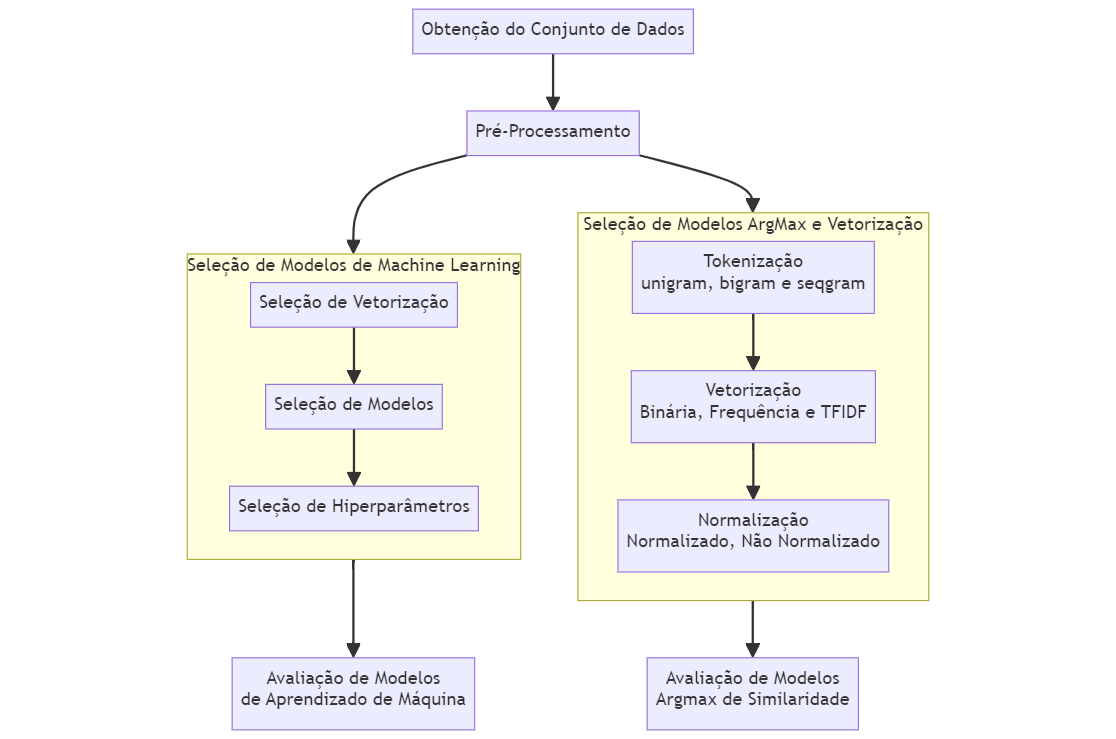
\includegraphics[width=0.8\textwidth]{images/fluxo.png}
    \caption{Fluxo de Trabalho.}
    \label{fig:workpipeline}
\end{figure}

\subsection{Conjunto de Dados}

O conjunto de dados foi obtido em \cite{dataset_2022}. Este conjunto de dados abrange descrições de produtos e suas respectivas categorias, coletadas dos dezoito maiores varejistas no Brasil, baseando-se na classificação da ABRAS do ano de 2020. Os itens selecionados representaram noventa e cinco por cento das vendas do ano de 2020 destes varejistas, representando os produtos mais vendidos das maiores redes varejistas do Brasil.

\subsubsection{Características Gerais}
O dataset é composto por 250.365 entradas e 7 colunas, detalhando descrições de produtos e informações taxonômicas. Os campos incluem \texttt{nm\_item}, \texttt{segmento}, \texttt{subsegmento}, \texttt{categoria}, \texttt{subcategoria}, \texttt{id\_product}, e \texttt{nm\_product}, todos categorizados como strings, exceto \texttt{id\_product} que é do tipo numérico. O número de valores únicos por coluna varia, indicando a diversidade dos produtos e sua classificação. Não existem registros nulos no dataset.

A tabela a seguir apresenta uma visão geral da estrutura hierárquica do conjunto de dados, destacando a organização e a especificidade com que os produtos são catalogados:

\begin{table}[h]
\centering
\begin{tabular}{ll}
\hline
\textbf{Nível de Classificação} & \textbf{Quantidade} \\
\hline
Segmentos              & 6          \\
Subsegmentos           & 20         \\
Categorias             & 70         \\
Subcategorias          & 169        \\
Categoria de Menor Nível & 795      \\
Descrições             & 250.365    \\
\hline
\end{tabular}
\caption{Visão geral da estrutura hierárquica do conjunto de dados.}
\label{table:estrutura_hierarquica}
\end{table}

\subsubsection{Detalhamento dos Campos e Hierarquia}

Para cada campo do conjunto de dados, é apresentado uma descrição a seguir:
\begin{itemize}
    \item \textbf{Nome do Item (\texttt{nm\_item})}: Este campo contém descrições dos produtos.
    \item \textbf{Segmento}: Funciona como uma classificação de nível superior, agrupando os produtos em categorias amplas. Com apenas seis categorias distintas, destaca uma divisão geral dos produtos.
    \item \textbf{Subsegmento}: Fornece uma subdivisão dos segmentos, oferecendo 20 categorias distintas para uma diferenciação mais detalhada entre os produtos.
    \item \textbf{Categoria}: Apresenta uma camada de classificação sob os subsegmentos com 70 categorias únicas.
    \item \textbf{Subcategoria}: Representa o quarto nível de classificação, com 169 subcategorias distintas.
    \item \textbf{Categoria de Nível Mais Baixo (\texttt{id\_product})}: Um código único atribuído a cada categoria de nível mais baixo, com 797 identificadores distintos, representa a menor granularidade hierárquica.
    \item \textbf{Descrição da Categoria de Nível Mais Baixo(\texttt{nm\_product})}: A descrição da categoria de menor granularidade hierárquica.
\end{itemize}

A estrutura hierárquica pode ser resumida na Figura \ref{fig:hierarquia}.
\begin{figure}[H]
    \centering
    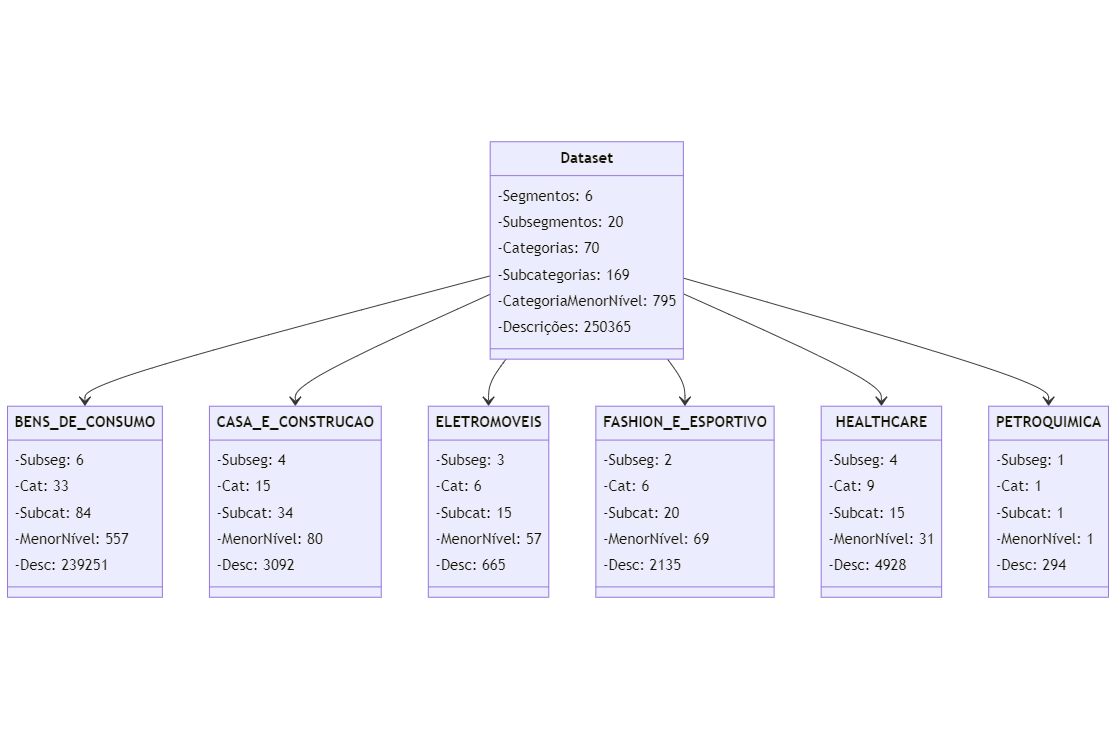
\includegraphics[width=0.8\textwidth]{images/hierarquia.png}
    \caption{Hierarquias}
    \label{fig:hierarquia e quantidade de elementos distintos e descrições em cada segmento}
\end{figure}


\subsubsection{Análise Exploratória de Dados (EDA)}

A Análise Exploratória de Dados é necessária para entender as características do conjunto de dados, permitindo a identificação de padrões, anomalias, e distribuições. As análises concentram-se em descrever características das descrições de produtos e a distribuição de rótulos pelas categorias de menor nível.

Inicia-se a análise pela distribuição das descrições pelas categorias utilizando a curva acumulada, figura \ref{fig:histdistclasses}.  A análise mostra que 70\% dos dados estão concentrados em 80 categorias de menor nível, indicando uma distribuição desigual. Este padrão ressalta a importância de algumas categorias no contexto dos varejistas.
\begin{figure}[H]
    \centering
    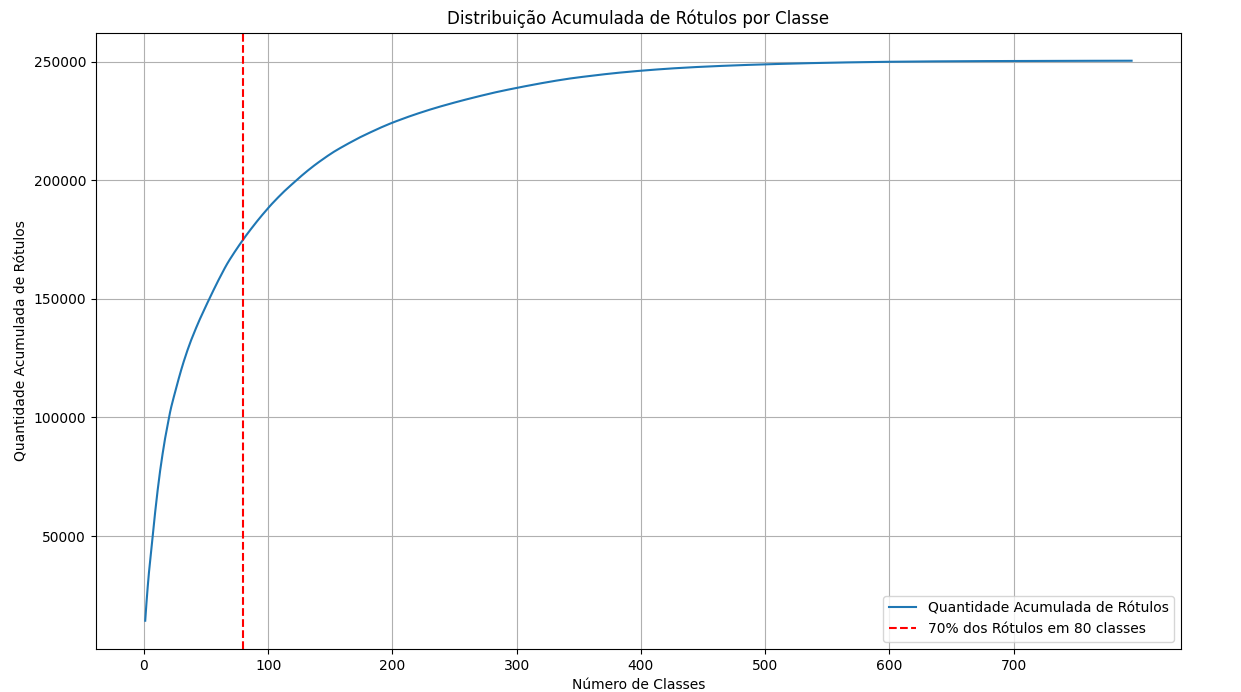
\includegraphics[width=0.8\textwidth]{images/histdistclasses.png}
    \caption{Distribuição das categorias de menor nível em escala logarítmica.}
    \label{fig:histdistclasses}
\end{figure}

Categorias como "BISCOITO" e "IOGURTE" lideram em quantidade de itens, refletindo as tendências de consumo. A Figura , Figura \ref{fig:grafico_barras_top10} exibe as 10 categorias com a maior quantidade de itens classificados.  Esta concentração denota o desbalanceamento e a dificuldade que se tem em tarefas de classificação.

 \begin{figure}[H]
    \centering
    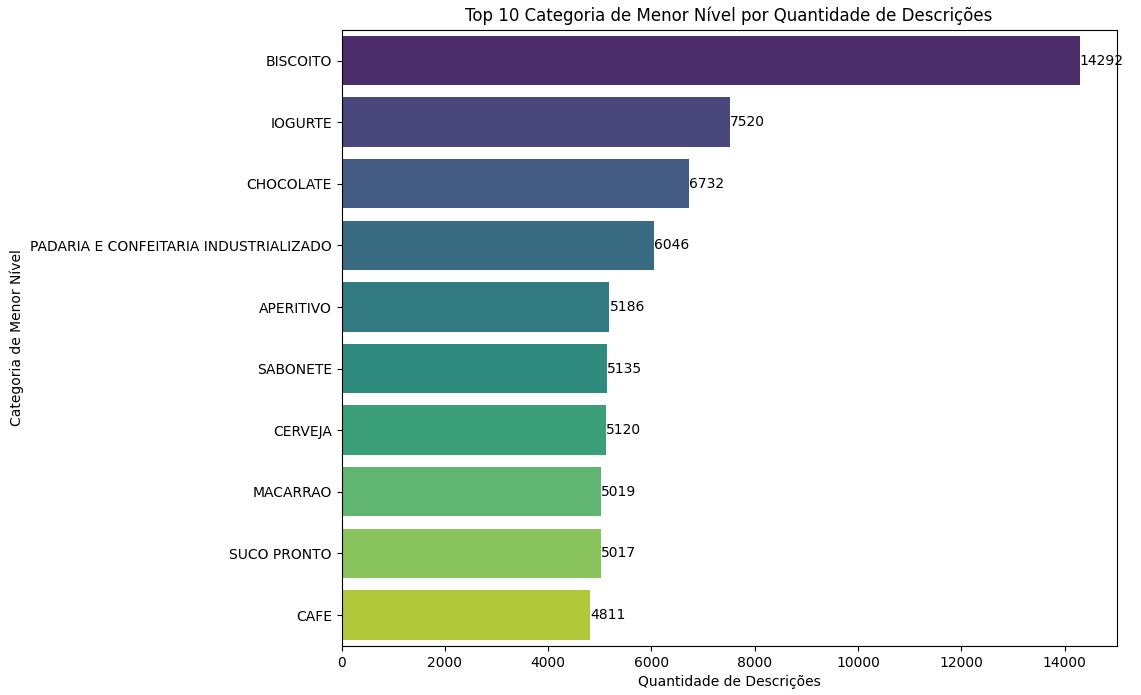
\includegraphics[width=0.8\textwidth]{images/grafico_barras_top10.png}
    \caption{Top 10 categorias de produtos com o maior número de rótulos.}
    \label{fig:grafico_barras_top10}
\end{figure}
\subsubsection{Análise Quantitativa das Descrições de Produtos}

Nesta seção é apresentada, como as descrições de produto se comportam nos varejos em relação a dois atributos importantes.  A quantidade de caracteres e quantidade de palavras.  Para definir uma palavra, realiza-se a segmentação da descrição por espaço.

\subsubsection{Distribuição de Caracteres por Descrição}
A Figura \ref{fig:distcaracteres} demonstra que maioria das descrições contém entre 20 a 35 caracteres, indicando uma preferência por descrições breves, mas informativas. Este padrão sugere que as descrições são projetadas para se encaixar dentro de cupons fiscais.  É interessante observar que não há nas descrições do dataset nenhum registro com mais de 50 caracteres, mostrando um padrão por descrições de até 50 caracteres.

\begin{figure}[H]
    \centering
    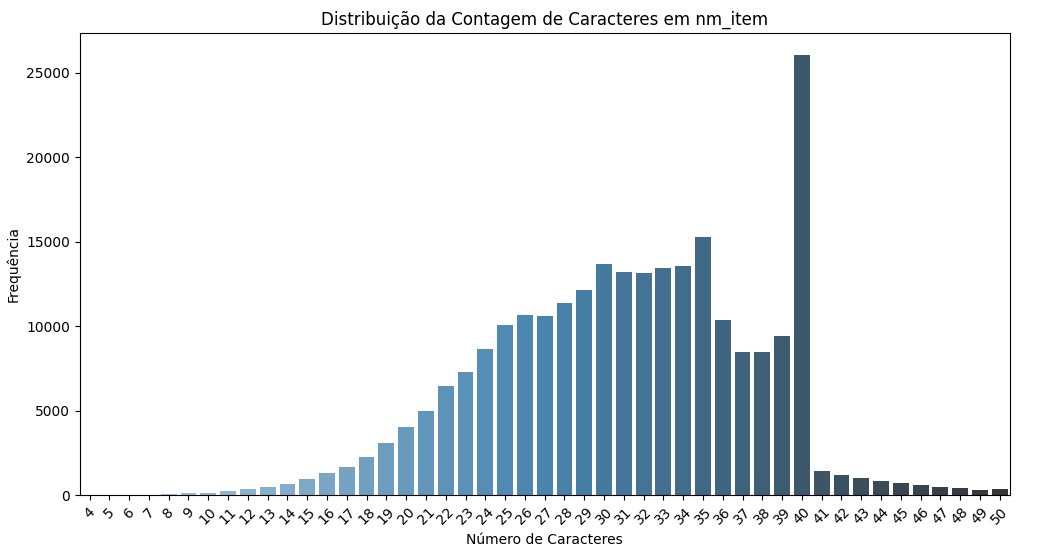
\includegraphics[width=0.8\textwidth]{images/distcaracteres.png}
    \caption{Distribuição de frequencia da contagem de caracteres por descrição.}
    \label{fig:distcaracteres}
\end{figure}

\subsubsection{Distribuição de Palavras por Descrição}
A Figura \ref{fig:distpalavras} apresenta a distribuição por palavra. Esta mostra uma predominância de descrições com 4 a 6 palavras, refletindo uma tendência à concisão nas descrições dos produtos. Este padrão é indicativo de um esforço para comunicar informações essenciais de forma eficiente, permitindo aos consumidores entender rapidamente as características dos produtos.

\begin{figure}[H]
    \centering
    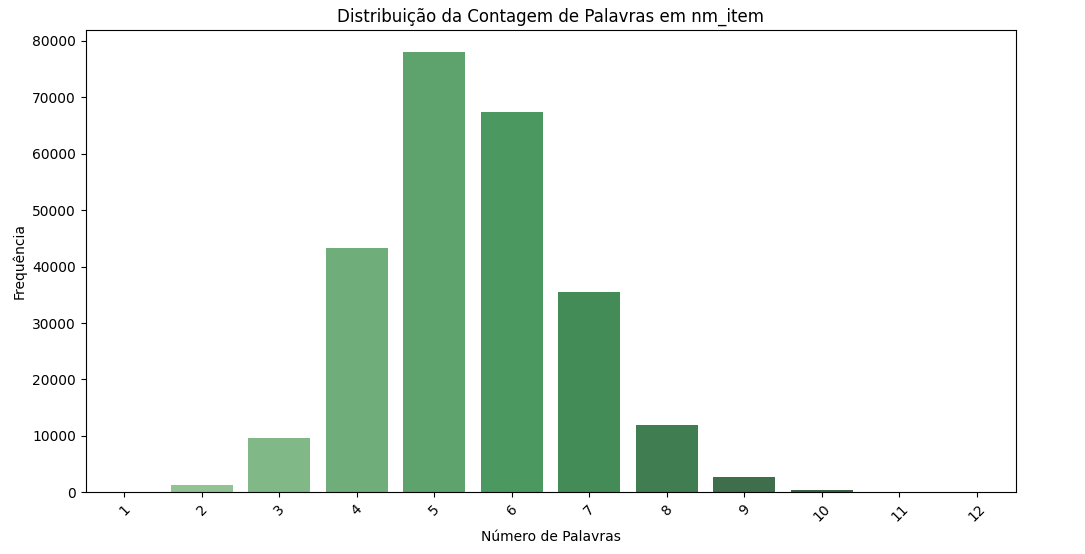
\includegraphics[width=0.8\textwidth]{images/distpalavrass.png}
    \caption{Distribuição de frequencia da contagem de palavras por descrição.}
    \label{fig:distpalavras}
\end{figure}

\subsection{Pré-Processamento}

Conforme discutido na seção \ref{subsec:preprocessamento}, a normalização, incluindo a remoção de acentos e a conversão para letras minúsculas, é adotada para uniformizar as variações linguísticas. Esta abordagem facilita a análise dos dados, alinhando-se com as práticas padrão em processamento de linguagem natural.  Diversas técnicas são apresentadas, mas as de maior impacto são a \textbf{normalização e conversão para minúsculas}.  As demais, conforme \cite{naseem2021survey}, acabam não impactando significativamente no resultado final.  Cabe ressaltar que as descrições de produto não apresentam verbos e variantes com prefixo e sufixo.

\subsection{Tokenização}
A tokenização é realizada para decompor os textos em unidades menores, ou tokens. Neste trabalho, serão exploradas representações baseadas em unigramas, bigramas e seqgramas. Esta decisão é fundamentada pela necessidade de capturar tanto a frequência de palavras individuais (\textit{unigramas}) quanto as relações entre palavras adjacentes (\textit{bigramas}) e sequências de palavras (\textit{seqgramas}), conforme destacado na seção \ref{subsec:tokenizacao}.

\subsection{Vetorização}
Utilizam-se as técnicas de Bag of Words (BoW), Term Frequency (TF), e Term Frequency-Inverse Document Frequency (TFIDF) para transformar os textos tokenizados em representações vetoriais. Estas técnicas são aplicadas a unigramas, bigramas e seqgramas, tanto em formas normalizadas quanto não-normalizadas, para capturar a importância relativa das palavras e suas relações contextuais.  Estas técnicas são descritas na seção \ref{subsec:representacaonumerica} sobre representação numérica.  A escolha se deve a ser os principais modelos utilizados pelas literaturas.

São avaliadas as representações vetoriais em suas formas normalizadas e não-normalizadas. A normalização dos vetores de características visa a padronização à uma escala comum, facilitando a integração de diferentes tipos de características e a aplicação de algoritmos de aprendizado de máquina.

\subsection{Seleção de Modelos}

Com base nos fundamentos apresentados anteriormente, a seleção de modelos para este estudo foi conduzida considerando-se as características distintas da classificação de textos curtos. Identificou-se que a natureza concisa dos dados demanda métodos capazes de extrair eficientemente a informação semântica limitada. Portanto, optou-se por avaliar tanto métodos de recuperação de informação, com ênfase no método baseado em similaridade, quanto modelos tradicionais de aprendizado de máquina, incluindo Naive Bayes (NB), Árvores de Decisão (DT), Máquinas de Vetores de Suporte (SVM), k-Nearest Neighbors (KNN) e Regressão Logística (RL).

\subsubsection{Argmax da Similaridade}

A adoção de métodos baseados em argmax para a classificação de texto neste estudo é justificada pela necessidade de um procedimento fundamentada na similaridade do conteúdo. Esses métodos servem como pontos iniciais para análises mais aprofundadas, proporcionando uma eficiente categorização preliminar de documentos. Além disso, a simplicidade desses métodos auxilia na interpretação dos resultados e na comparação com abordagens mais complexas, estabelecendo uma base sólida para a exploração de métodos adicionais.

\paragraph{Vantagens e Desvantagens}
\textbf{Vantagens:}
\begin{itemize}
    \item Simplicidade de Implementação: Facilita a compreensão e a implementação.
    \item Eficiência Computacional: Permite execução rápida, especialmente em conjuntos de dados volumosos.
    \item Adaptabilidade: Aplica-se a diferentes métricas de similaridade.
\end{itemize}

\textbf{Desvantagens:}
\begin{itemize}
    \item Sensibilidade a Distorções nos Dados: Vulnerabilidade a ruídos e outliers.
    \item Desconsideração da Distribuição de Similaridade: Foco exclusivo no valor máximo, ignorando a distribuição global de similaridades.
    \item Limitação em Contextos Complexos: Dificuldade em capturar nuances em textos com múltiplas interpretações ou categorias próximas.
\end{itemize}

\subsubsection{Modelos Tradicionais}
\begin{itemize}
    \item \textbf{Naive Bayes (NB):} Selecionado pela sua eficiência e simplicidade, reconhecido por sua robustez na classificação de texto.
    
    \item \textbf{Árvores de Decisão (DT):} Escolhidas pela capacidade de abordar características não lineares e pela facilidade de interpretação dos modelos gerados.
    
    \item \textbf{Máquinas de Vetores de Suporte (SVM):} A eficácia em espaços de alta dimensão motivou sua seleção.
    
    \item \textbf{k-Nearest Neighbors (KNN):} A simplicidade e eficácia em classificações que não demandam modelos complexos foram as principais razões para sua escolha.
    
    \item \textbf{Regressão Logística (RL):} Incluída por sua habilidade em fornecer probabilidades de classe, útil para classificar descrições ambíguas.
\end{itemize}

\paragraph{Considerações}
A exclusão de modelos de aprendizado profundo, técnicas de bagging e boosting, bem como modelos baseados em word embeddings, foi uma decisão intencional, motivada pela limitação de escopo deste trabalho. Esta pesquisa estabelece uma fundação inicial, focando em métodos tradicionais e de recuperação de informação, pavimentando o caminho para futuros estudos que possam explorar métodos mais avançados e contemporâneos. A diversidade dos modelos selecionados permite uma avaliação abrangente das técnicas de classificação de texto, maximizando as chances de identificar o método mais eficaz para o conjunto de dados específico.

\subsection{Métricas de Avaliação}

O principal objetivo das métricas de avaliação é fornecer um quadro confiável para a análise do desempenho dos modelos. Procurou-se selecionar métricas que considerassem tanto a eficácia geral do modelo quanto sua capacidade de tratar classes de maneira equitativa, evitando viés em favor das classes mais representativas no conjunto de dados.  Desta forma, pode-se resumir o objetivo em \textit{abrangência} e \textit{equidade}.  Segundo Tharwat (2018) e Grandini et al. (2020), as métricas são fundamentais para compreender o desempenho dos modelos em contextos multiclasse, onde a complexidade e o desbalanceamento entre classes apresentam desafios significativos.
Para satisfazer estes dois critérios foram escolhidas a \textbf{F1-Score Macro} e \textbf{Acurácia}. Elas juntas proporcionam uma visão equilibrada e abrangente do desempenho dos modelos.
Quanto a \textbf{abrangência} a acurácia fornece uma visão geral do desempenho enquanto que para a \textbf{equidade} A F1-score macro, ao calcular a média dos F1-Scores de todas as classes, dá igual peso a cada uma delas, favorecendo uma avaliação justa independentemente do tamanho da classe.

\subsection{Configurações de Treinamento}

Para avaliar o desempenho dos modelos de aprendizado de máquina especificados neste estudo, o conjunto de dados foi submetido a um processo de randomização antes da aplicação das técnicas de treinamento. A técnica de validação cruzada k-fold com 10 partições foi adotada, baseando-se na recomendação de \cite{kohavi1995study}, que destaca a eficiência desta abordagem em proporcionar estimativas confiáveis do desempenho dos modelos.

O procedimento foi realizado da seguinte forma: após a randomização do conjunto de dados, este foi dividido em 10 partições de tamanho igual. Utilizando a abordagem de validação cruzada, em cada ciclo, nove partições foram empregadas para o treinamento do modelo, enquanto a partição restante foi reservada para teste. Este processo foi repetido 10 vezes, com cada partição servindo exatamente uma vez como conjunto de teste. Essa metodologia assegura uma avaliação completa e equitativa do desempenho dos modelos avaliados no trabalho.

\subsection{Ajuste Fino dos Modelos}

O ajuste fino dos hiperparâmetros visa otimizar o desempenho dos modelos de aprendizado de máquina. Nesta seção, é descrito os hiperparâmetros que serão avaliados para cada modelo utilizado neste estudo.

\subsubsection{Métodos Baseados em Argmax}

Para os métodos baseados em argmax, as combinações dos seguintes hiperparâmetros serão avaliadas:

\begin{itemize}
    \item \textbf{Tokenização}: Serão exploradas três abordagens distintas para a tokenização: unigramas, bigramas e seqgramas. Essas abordagens permitem analisar a influência do tamanho dos tokens na performance do modelo.
    \item \textbf{Vetorização}: É avaliada três técnicas de vetorização: binária, frequência e TF-IDF (Term Frequency-Inverse Document Frequency). Cada técnica fornece uma representação diferente dos textos, que será examinada em termos de impacto no desempenho do modelo.
    \item \textbf{Normalização}: Será considerada a aplicação ou não de normalização nos textos, incluindo a conversão para minúsculas e remoção de acentos, para verificar sua influência na eficácia do modelo.
\end{itemize}

A combinação desses hiperparâmetros visa explorar uma ampla gama de configurações para identificar aquela que proporciona o melhor desempenho para a classificação de texto baseada em argmax. A tabela \ref{tab:combinacoes} exibe as combinações avaliadas.

\begin{table}[H]
\centering
\caption{Combinações de Tokenização, Vetorização e Normalização}
\label{tab:combinacoes}
\begin{tabular}{l|l|l|l}
\hline
\textbf{ID} & \textbf{Tokenização} & \textbf{Tipo} & \textbf{Normalização} \\ \hline
ARGMAX1BI            & unigram     & Binário &               \\ \hline
ARGMAX1BINORM        & unigram     & Binário & Normalizado   \\ \hline
ARGMAX1TF            & unigram     & TF      &               \\ \hline
ARGMAX1TFNORM        & unigram     & TF      & Normalizado   \\ \hline
ARGMAX1TFIDF         & unigram     & TFIDF   &               \\ \hline
ARGMAX1TFIDFNORM     & unigram     & TFIDF   & Normalizado   \\ \hline
ARGMAX2BI            & bigram      & Binário &               \\ \hline
ARGMAX2BINORM        & bigram      & Binário & Normalizado   \\ \hline
ARGMAX2TF            & bigram      & TF      &               \\ \hline
ARGMAX2TFNORM        & bigram      & TF      & Normalizado   \\ \hline
ARGMAX2TFIDF         & bigram      & TFIDF   &               \\ \hline
ARGMAX2TFIDFNORM     & bigram      & TFIDF   & Normalizado   \\ \hline
ARGMAXSBI            & seqgram     & Binário &               \\ \hline
ARGMAXSBINORM        & seqgram     & Binário & Normalizado   \\ \hline
ARGMAXSTF            & seqgram     & TF      &               \\ \hline
ARGMAXSTFNORM        & seqgram     & TF      & Normalizado   \\ \hline
ARGMAXSTFIDF         & seqgram     & TFIDF   &               \\ \hline
ARGMAXSTFIDFNORM     & seqgram     & TFIDF   & Normalizado   \\ \hline
\end{tabular}
\end{table}

\subsubsection{Modelos de Aprendizado de Máquina}

O processo de ajuste fino para os modelos de aprendizado de máquina específicos será detalhado a seguir, focando nos hiperparâmetros chave de cada um:

\paragraph{Máquina de Vetores de Suporte (SVM)}

A Máquina de Vetores de Suporte (SVM) é um modelo de aprendizado de máquina baseado em otimização, projetado para encontrar um hiperplano que minimize a distância até os vetores mais próximos de classes distintas, conhecidos como vetores de suporte. A formulação matemática do SVM é expressa pela seguinte equação, adaptada de \cite{pedregosa2011scikit}:

\begin{equation}
\label{eq6}
\begin{aligned}\min_ {w, b, \zeta} \frac{1}{2} w^T w + C \sum_{i=1}^{n} \zeta_i\\
\begin{split}\textrm {sujeito a} \\
& y_i (w^T \phi (x_i) + b) \geq 1 - \zeta_i,\\
& \zeta_i \geq 0, i=1, ..., n\end{split}
\end{aligned}
\end{equation}

Durante o processo de ajuste fino, os seguintes hiperparâmetros do SVM serão avaliados:

\begin{itemize}
    \item \textbf{Funções de Kernel:} Diferentes funções de kernel, incluindo linear, polinomial, radial (RBF) e sigmoide, serão testadas. O kernel transforma o espaço de entrada em um espaço de maior dimensão onde é possível encontrar um hiperplano de separação linear.
    \item \textbf{C (Parâmetro de Regularização):} O parâmetro C, que controla o trade-off entre a maximização da margem e a minimização do erro de classificação, será ajustado. Valores mais altos de C indicam uma menor tolerância a erros de classificação.
    \item \textbf{Peso da Classe:} Este hiperparâmetro ajusta o peso das classes, sendo particularmente útil em situações de desbalanceamento de classes.
    \item \textbf{Grau (para Kernel Polinomial):} Quando o kernel polinomial é selecionado, o grau do polinômio representa um hiperparâmetro crítico que será ajustado.
\end{itemize}

A seleção e o ajuste desses hiperparâmetros serão realizados por meio de técnicas como busca em grade (Grid Search) ou busca aleatória (Random Search), com o objetivo de identificar a configuração que maximiza a precisão do modelo SVM no conjunto de dados utilizado neste estudo.

\paragraph{Regressão Logística}

A Regressão Logística (RL) é empregada como um modelo de classificação no contexto de aprendizado de máquina supervisionado. A formulação matemática da RL, adaptada de \cite{pedregosa2011scikit}, é apresentada abaixo:

\begin{equation}
\label{eq5}
\min_{w, c} \frac{1 - \rho}{2}w^T w + \rho \|w\|_1 + \\ C \sum_{i=1}^n \\ \log\left (e^{-y_i (X_i^T w + c)} + 1\right )
\end{equation}

Durante o ajuste fino, os seguintes hiperparâmetros da Regressão Logística serão explorados:

\begin{itemize}
    \item \textbf{Solver:} O método de otimização a ser utilizado na minimização da função de custo. O solver "saga" foi escolhido por sua eficiência em conjuntos de dados de grande escala.
    \item \textbf{Penalidade (Penalty):} Representa o tipo de regularização aplicada ao modelo. Serão testadas as opções "l1" (norma L1), "l2" (norma L2) e "elasticnet", que é uma combinação linear das penalidades L1 e L2. A relevância de cada tipo de penalidade será determinada pelo ajuste do hiperparâmetro \(\rho\) (l1\_ratio) no caso de "elasticnet".
    \item \textbf{C (Parâmetro de Regularização):} Controla a força da regularização inversamente. Valores mais altos de C correspondem a uma regularização menos rigorosa. Serão avaliados diferentes valores de C para identificar o equilíbrio ideal entre bias e variância.
    \item \textbf{Peso da Classe (Class Weight):} Este hiperparâmetro ajusta os pesos das classes no cálculo da função de custo, sendo particularmente útil em situações com classes desbalanceadas. A opção "balanceada" será comparada ao cenário onde todas as classes têm o mesmo peso.
\end{itemize}

O processo de ajuste desses hiperparâmetros visa otimizar o desempenho da Regressão Logística no conjunto de dados estudado, utilizando técnicas como busca em grade (Grid Search) para explorar o espaço de hiperparâmetros de forma sistemática.

\paragraph{Árvores de Decisão}

As Árvores de Decisão são modelos de aprendizado de máquina supervisionado amplamente utilizados para tarefas de classificação e regressão. Esses modelos são preferidos por sua facilidade de interpretação, a capacidade de lidar com dados não lineares e a não necessidade de normalização dos dados. A formulação matemática específica para uma árvore de decisão é mais intuitiva, focando na divisão do espaço de dados em regiões homogêneas com base nos valores dos atributos.

Durante o processo de ajuste fino, os seguintes hiperparâmetros das Árvores de Decisão serão avaliados:

\begin{itemize}
    \item \textbf{Critério:} O critério utilizado para medir a qualidade de uma divisão. Os critérios mais comuns são "gini" para a impureza de Gini e "entropy" para o ganho de informação (entropia), sendo ambos avaliados para determinar qual oferece o melhor desempenho para o modelo.
    \item \textbf{Profundidade Máxima da Árvore (max\_depth):} A profundidade máxima da árvore será ajustada para controlar a complexidade do modelo, prevenindo overfitting. Serão testados valores variados para encontrar o equilíbrio ideal entre bias e variância.
    \item \textbf{Número Mínimo de Amostras para Dividir um Nó (min\_samples\_split):} Este hiperparâmetro determina o número mínimo de amostras necessárias para dividir um nó interno. Valores diferentes serão explorados para otimizar a capacidade da árvore de generalizar bem para dados não vistos.
    \item \textbf{Número Mínimo de Amostras em um Nó Folha (min\_samples\_leaf):} O número mínimo de amostras requeridas para estar em um nó folha. Ajustar esse parâmetro ajuda a suavizar o modelo, especialmente em casos de dados ruidosos.
\end{itemize}

O ajuste desses hiperparâmetros será realizado por meio de técnicas de busca, como a busca em grade (Grid Search) ou busca aleatória (Random Search), com o objetivo de identificar a configuração que maximiza a precisão da árvore de decisão no conjunto de dados utilizado neste estudo.

\paragraph{k-Nearest Neighbors (KNN)}

O k-Nearest Neighbors (KNN) é um algoritmo simples, porém poderoso, utilizado tanto para classificação quanto para regressão. Baseia-se no princípio de que as amostras mais próximas no espaço de características tendem a pertencer à mesma classe. O KNN é particularmente apreciado por sua facilidade de implementação e sua eficácia em uma ampla gama de problemas.

Durante o processo de ajuste fino, os seguintes hiperparâmetros do KNN serão avaliados:

\begin{itemize}
    \item \textbf{Número de Vizinhos (n\_neighbors):} O número de vizinhos a considerar determina a fronteira de decisão do KNN. Serão testados diferentes valores para encontrar o número ótimo de vizinhos que maximiza a precisão do modelo.
    \item \textbf{Peso dos Vizinhos (weights):} O peso atribuído aos vizinhos pode ser uniforme, onde todos os vizinhos contribuem igualmente, ou baseado na distância, onde vizinhos mais próximos têm uma influência maior na decisão. Ambas as opções serão exploradas para determinar qual oferece o melhor desempenho.
    \item \textbf{Métrica de Distância (metric):} A escolha da métrica de distância (como distância euclidiana, manhattan, minkowski, ou hamming) é crucial para o desempenho do KNN. Diferentes métricas serão avaliadas para identificar a mais adequada para o conjunto de dados em questão.
    \item \textbf{Algoritmo para Computação da Distância (algorithm):} As opções incluem 'ball\_tree', 'kd\_tree', 'brute', e 'auto', influenciando a eficiência do cálculo das distâncias. O algoritmo mais eficiente para o nosso conjunto de dados será identificado mediante experimentação.
\end{itemize}

O processo de ajuste desses hiperparâmetros será conduzido utilizando técnicas como a busca em grade (Grid Search) ou busca aleatória (Random Search), visando encontrar a configuração que oferece o melhor equilíbrio entre precisão e eficiência computacional para o modelo KNN no conjunto de dados utilizado neste estudo.

\paragraph{Naive Bayes}

O Naive Bayes é um classificador probabilístico baseado no teorema de Bayes, com a "ingênua" suposição de independência entre os preditores. Apesar de sua simplicidade, o Naive Bayes pode ser surpreendentemente eficaz e é frequentemente utilizado em tarefas de classificação de texto e filtragem de spam.

No ajuste fino do modelo Naive Bayes, focaremos na seleção do tipo de modelo Naive Bayes apropriado para o nosso conjunto de dados, uma vez que diferentes variantes são mais adequadas para diferentes tipos de distribuição de dados. Os seguintes hiperparâmetros e variantes do modelo serão avaliados:

\begin{itemize}
    \item \textbf{Tipo de Modelo Naive Bayes:} Dependendo da natureza do conjunto de dados, diferentes versões do Naive Bayes serão testadas, incluindo:
    \begin{itemize}
        \item Gaussian Naive Bayes: Ideal para características com distribuição normal.
        \item Multinomial Naive Bayes: Adequado para dados distribuídos multinomialmente, como a contagem de palavras em textos.
        \item Bernoulli Naive Bayes: Utilizado para características binárias/multivariáveis.
        \item Complement Naive Bayes: Uma adaptação do Multinomial Naive Bayes que é particularmente adequada para conjuntos de dados desbalanceados.
    \end{itemize}
    \item \textbf{Suavização Laplaciana (alpha):} Para modelos como Multinomial e Bernoulli Naive Bayes, a suavização Laplaciana (ou aditiva) é aplicada para lidar com o problema de probabilidade zero. O valor de $\alpha$ será ajustado para otimizar o desempenho do modelo.
\end{itemize}

A seleção do modelo e o ajuste do hiperparâmetro de suavização serão realizados por meio de validação cruzada, com o objetivo de identificar a configuração que oferece a melhor acurácia para a classificação no conjunto de dados estudado.




\chapter{Resultados}

\section{Introdução aos Resultados}

Neste capítulo, os resultados obtidos a partir da aplicação dos métodos de classificação de texto analisados neste estudo são apresentados, incluindo tanto técnicas baseadas em Argmax. A avaliação do desempenho desses métodos é considerada referencial para compreender sua eficácia na classificação de descrições de produtos em português, utilizando o dataset RETAILPRODUCTDESCRIPTION-PTBR especialmente preparado para este fim.

Inicialmente, uma análise detalhada dos resultados obtidos com o método Argmax é apresentada, explorando diferentes configurações de vetorização, tokenização e normalização, e como estas são vistas para afetar o desempenho do método em termos de acurácia e F1-Score Macro.

Finalmente, uma comparação geral dos resultados de todos os métodos analisados é realizada, oferecendo uma visão integrada do desempenho relativo de cada técnica. Esta seção de resultados gerais visa identificar os métodos mais promissores provenientes das técnicas base da recuperação da informação para a classificação de textos curtos em português, considerando as particularidades do dataset em estudo. Discussões sobre as limitações dos resultados, considerações para a interpretação dos dados e sugestões para pesquisas futuras também são abordadas, fornecendo um panorama dos achados e sua implicação para o campo do processamento de linguagem natural e aprendizado de máquina.

\subsection{Avaliação do Método Argmax}

Para a avaliação do método Argmax, diversas combinações de parâmetros foram examinadas. O foco desta análise reside na determinação de configurações ótimas que apresentam a melhor combinação de acurácia e f1score macro na tarefa de classificação de textos curto, especificamente nas descrições de produtos em português. As combinações de parâmetros selecionadas para estudo incluem:

As combinações de parâmetros selecionadas para o estudo foram:

\begin{itemize}
    \item \textbf{Método de Vetorização:} Foram consideradas abordagens binárias, frequência de termos (TF) e frequência de termos ponderada pelo inverso da frequência dos termos nos documentos (TF-IDF).
    \item \textbf{N-Gramas:} Unigramas (1,1) e unigramas com bigramas (1,2) foram avaliados.
    \item \textbf{Normalização:} A influência da normalização L2 foi examinada em comparação com a ausência de normalização.
\end{itemize}

Para uma compreensão completa do desempenho e da eficácia das diferentes configurações avaliadas, a análise será iniciada examinando os resultados das medidas de acurácia e F1 Score Macro para todas as combinações de parâmetros. Uma tabela detalhada será apresentada, incluindo o ranqueamento de cada método em cada medida, proporcionando uma visão abrangente do desempenho relativo de cada configuração. Em seguida, boxplots serão utilizados para visualizar a distribuição das medidas de acurácia e F1 Score Macro, destacando possíveis padrões e variações entre as configurações. Complementando esta análise, um gráfico bidimensional, denominado "Gráfico de Desempenho", será apresentado, ilustrando a relação entre acurácia (eixo x) e F1 Score Macro (eixo y) para cada configuração avaliada. Posteriormente, uma análise detalhada do impacto da tokenização e normalização em cada método será conduzida, identificando as configurações mais promissoras e destacando os pontos fortes e fracos de cada abordagem. Por fim, com base nos insights obtidos, recomendações serão oferecidas sobre as melhores práticas para a seleção de parâmetros e a configuração ideal do método Argmax em tarefas de classificação de texto em português.

\subsubsection{Resultados}

    Foram realizadas simulações com todas as combinações utilizando para testre e treino o método K-Fold com 10 partições.  Isto permite gerar estatísticas e avaliar a variância do método, aqui avaliada em porcentagem pelo coeficiente de variação.  A tabela \ref{tab:resultadoargmax_rankings} apresenta estas estatísticas.

\begin{table}[H]
\centering
\caption{Resultados estatísticos dos testes para o método Argmax com Rankings}
\label{tab:resultadoargmax_rankings}
\footnotesize % Diminui a fonte da tabela
\begin{tabular}{lllrrrrrr}
\hline
Método & NGram & Norm & \multicolumn{3}{c}{Acurácia (\%)} & \multicolumn{3}{c}{F1 Score Macro(\%)} \\
& & & Média & CV & \# & Média & CV & \# \\
\hline
Binary & [1, 1] & None & 75.31 & 0.44 & 6 & 58.77 & 3.15 & 3 \\
Binary & [1, 1] & L2 & 19.07 & 2.40 & 12 & 25.39 & 2.04 & 11 \\
Binary & [1, 2] & None & 89.56 & 0.21 & 1 & 70.09 & 1.91 & 1 \\
Binary & [1, 2] & L2 & 31.30 & 1.48 & 11 & 33.82 & 1.77 & 8 \\
TermFrequency & [1, 1] & None & 63.76 & 0.41 & 10 & 23.44 & 2.05 & 12 \\
TermFrequency & [1, 1] & L2 & 77.05 & 0.24 & 4 & 52.31 & 2.46 & 5 \\
TermFrequency & [1, 2] & None & 66.68 & 0.28 & 9 & 27.08 & 1.69 & 10 \\
TermFrequency & [1, 2] & L2 & 79.65 & 0.29 & 3 & 55.56 & 2.61 & 4 \\
TFIDF & [1, 1] & None & 70.64 & 0.28 & 8 & 32.10 & 2.25 & 9 \\
TFIDF & [1, 1] & L2 & 78.37 & 0.32 & 5 & 55.20 & 2.47 & 6 \\
TFIDF & [1, 2] & None & 74.57 & 0.33 & 7 & 37.67 & 1.53 & 7 \\
TFIDF & [1, 2] & L2 & 82.76 & 0.29 & 2 & 59.83 & 2.52 & 2 \\
\hline
\end{tabular}
\end{table}

\subsection{Análise dos Resultados}

\subsubsection{Acurácia}

Os resultados de acurácia revelam que o método Binary com NGram [1, 2] e sem normalização obteve a maior média de acurácia (89.56\%), seguido pelo método TFIDF com NGram [1, 2] e L2 (82.76\%). Por outro lado, o método Binary com NGram [1, 1] e L2 apresentou a menor média de acurácia (19.07\%). Observa-se que o método Binary com NGram [1, 1] e L2 apresentou o maior coeficiente de variação (CV) (2.40\%), indicando uma maior variabilidade nos resultados.

Os boxplots das acurácias (Figura \ref{fig:boxplot_acuracia}) demonstram uma variância relativamente baixa entre as combinações de parâmetros testadas. Observou-se a presença de poucos outliers, indicando que a maioria das configurações apresenta um desempenho consistente. As combinações que utilizam o método binário sem normalização destacaram-se por apresentar as melhores acurácias, enquanto aquelas com normalização L2 mostraram-se menos eficazes.
\begin{figure}[H]
    \centering
    \includegraphics[width=0.8\textwidth]{images/ArgmaxAcuráciaTodos.png}
    \caption{Boxplot das acurácias das combinações Argmax.}
    \label{fig:boxplot_acuracia}
\end{figure}

\subsubsection{F1 Score Macro}


Em relação ao F1 Score Macro, observa-se algumas diferenças em comparação com os resultados de acurácia. Por exemplo, o método Binary com NGram [1, 2] e sem normalização mantém sua posição de destaque, enquanto o método TFIDF com NGram [1, 1] e L2 apresenta um desempenho superior em relação ao método TermFrequency com a mesma configuração. As diferenças nos rankings atribuídos para acurácia e F1 Score destacam a importância de considerar múltiplas métricas ao avaliar o desempenho de modelos de classificação de texto.

Similarmente, os boxplots dos F1 Scores Macro (Figura \ref{fig:boxplot_f1score}) revelam que as configurações com bom desempenho em acurácia tendem também a exibir resultados satisfatórios no F1 Score Macro. Este padrão sugere que as configurações selecionadas são capazes de manter um equilíbrio razoável na performance entre as diversas classes, mesmo considerando o desbalanceamento presente no conjunto de dados.

\begin{figure}[H]
    \centering
    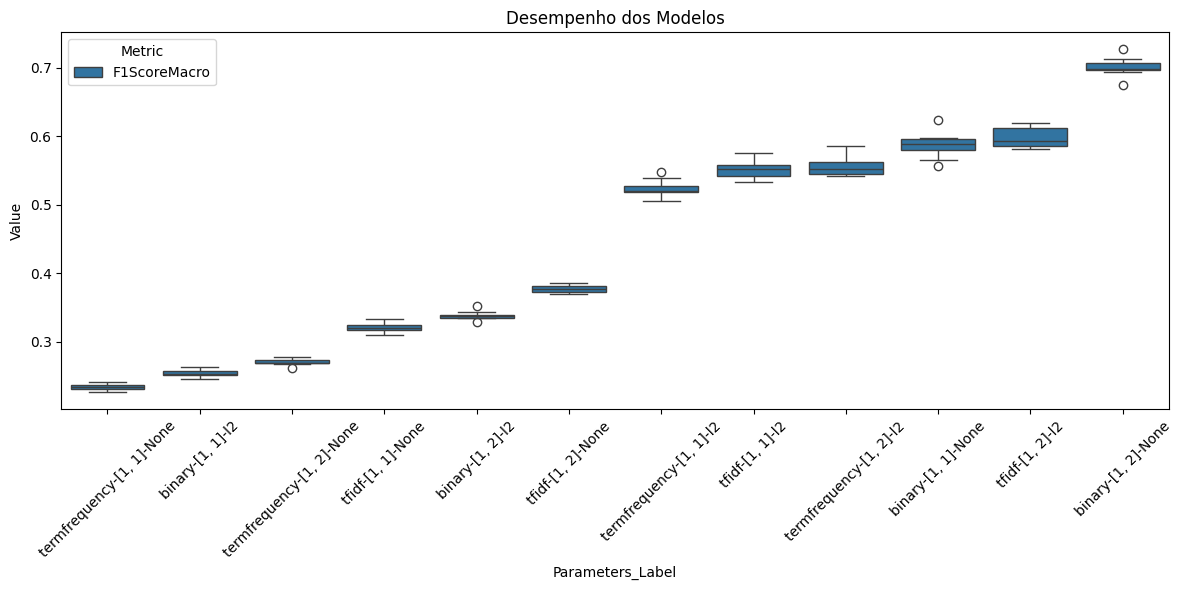
\includegraphics[width=0.8\textwidth]{images/ArgmaxF1ScoreTodos.png}
    \caption{Boxplot dos F1 Scores Macro das combinações Argmax.}
    \label{fig:boxplot_f1score}
\end{figure}

\subsubsection{Análise Combinada}

\subsection{Análise do Gráfico de Métricas Combinadas}

A análise combinada dos resultados visa integrar as observações feitas individualmente para acurácia e F1 Score Macro, oferecendo uma visão geral do desempenho dos métodos de classificação utilizados. Esta seção enfoca a interpretação conjunta dessas métricas, utilizando o gráfico de dispersão para ilustrar a eficácia relativa de cada configuração de método de vetorização, n-gramas e normalização.

O gráfico de dispersão apresentado na Figura \ref{fig:scatter_acuracia_f1score_ilustracao} permite uma análise visual das diferentes configurações de modelos de classificação, dividindo o espaço em quatro áreas distintas. Na área superior direita (++), encontram-se as configurações que alcançaram altos valores tanto de acurácia quanto de F1 Score Macro, indicando um desempenho superior em ambas as métricas. Por outro lado, na área inferior esquerda (--), situam-se as combinações que apresentaram os piores resultados em ambas as métricas. Na área superior esquerda (-+), estão as configurações que alcançaram baixa acurácia, mas alto F1 Score Macro, enquanto na área inferior direita (+-), encontram-se as combinações com alta acurácia e baixo F1 Score Macro. Isto fornece uma maneira de avaliar ambas as métricas ao mesmo tempo.


\begin{figure}[htbp]
    \centering
    \begin{tikzpicture}
    \begin{axis}[
        xlabel={Acurácia},
        ylabel={F1 Score Macro},
        xmin=0, xmax=100,
        ymin=0, ymax=100,
        xtick={0,20,40,60,80,100},
        ytick={0,20,40,60,80,100},
        legend pos=north west,
        grid style=dashed,
    ]
    
    \draw[dotted] (50,0) -- (50,100);
    \draw[dotted] (0,50) -- (100,50);
    
    \addplot[
        only marks,
        mark=*,
        blue,
        mark options={scale=1.5},
        nodes near coords,
        point meta=explicit symbolic,
    ] table[meta=label] {
    x y label
    25 75 [-,+]
    75 75 [+,+]
    25 25 [-,-]
    75 25 [+,-]
    };
    \legend{Configurações}
    \end{axis}
    \end{tikzpicture}
\caption{Interpretação do gráfico de dispersão relacionando acurácia e F1 Score Macro das combinações Argmax.}
    \label{fig:scatter_acuracia_f1score_ilustracao}
\end{figure}

No gráfico \ref{fig:scatter_acuracia_f1score} apresenta-se os métodos de maneira combinada.  Isto permite separar os métodos em quatro grupos distintos de configurações, divididos conforme a mediana de cada métrica. 

\begin{itemize}
    \item \textbf{Quadrante Superior Direito (++)}: Configurações com alto desempenho tanto em acurácia quanto em F1 Score Macro.
    \begin{itemize}
        \item Binary [1, 2] \& None: Acurácia = 89.56\%, F1 Score Macro = 70.09\%.
        \item TermFrequency [1, 2] \& L2: Acurácia = 79.65\%, F1 Score Macro = 55.56\%.
        \item TFIDF [1, 2] \& L2: Acurácia = 82.76\%, F1 Score Macro = 59.83\%.
        \item Binary [1, 1] \& None: Acurácia = 75.31\%, F1 Score Macro = 58.77\%.
        \item TermFrequency [1, 1] \& L2: Acurácia = 77.05\%, F1 Score Macro = 52.31\%.
        \item TFIDF [1, 1] \& L2: Acurácia = 78.37\%, F1 Score Macro = 55.20\%.
    \end{itemize}

    \item \textbf{Quadrante Inferior Direito (+-)}: Configurações com alta acurácia mas F1 Score Macro abaixo de 50\%.
    \begin{itemize}
        \item TFIDF [1, 1] \& None: Acurácia = 70.64\%, F1 Score Macro = 32.10\%.
        \item TFIDF [1, 2] \& None: Acurácia = 74.57\%, F1 Score Macro = 37.67\%.
        \item TermFrequency [1, 1] \& None: Acurácia = 63.76\%, F1 Score Macro = 23.44\%.
        \item TermFrequency [1, 2] \& None: Acurácia = 66.68\%, F1 Score Macro = 27.08\%.
    \end{itemize}

    \item \textbf{Quadrante Inferior Esquerdo (--) }: Configurações com desempenho abaixo de 50\% em ambas as métricas.
    \begin{itemize}
        \item Binary [1, 1] \& L2: Acurácia = 19.07\%, F1 Score Macro = 25.39\%.
        \item Binary [1, 2] \& L2: Acurácia = 31.30\%, F1 Score Macro = 33.82\%.
    \end{itemize}

    \item \textbf{Quadrante Superior Esquerdo (-+)}: Não aplicável, pois não há configurações com acurácia < 50\% e F1 Score Macro >= 50\%.
\end{itemize}

Concluída a classificação preliminar das configurações por meio do método Argmax, a investigação avança para uma avaliação detalhada de cada técnica de classificação textual individualmente. Esta etapa visa avaliar o impacto dos parâmetros específicos — incluindo o método de vetorização, a aplicação de N-Gramas e a normalização — na acurácia e no F1 Score Macro associados a cada método.

\begin{figure}[H]
    \centering
    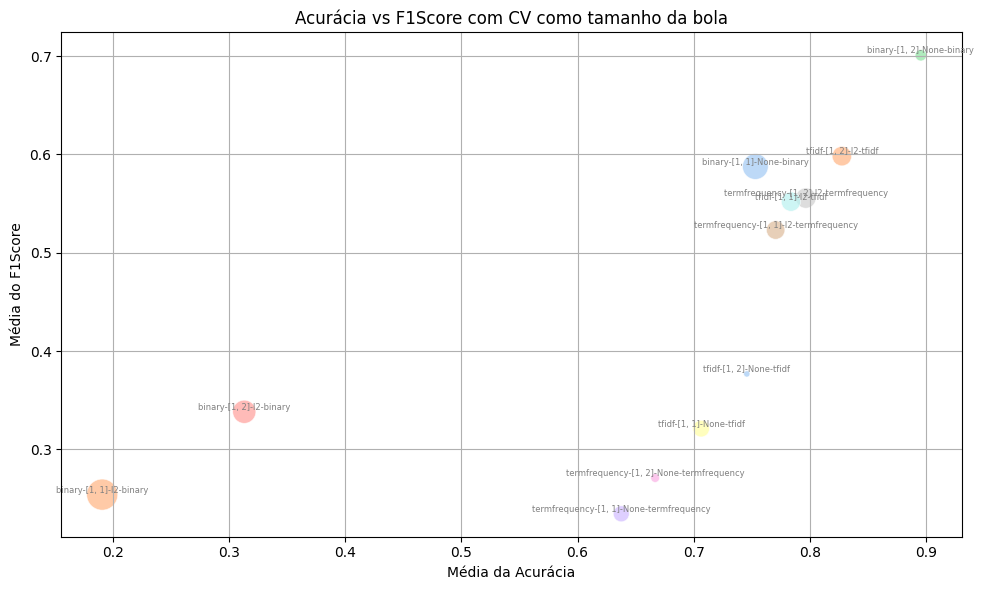
\includegraphics[width=0.8\textwidth]{images/ArgmaxScatterTodos.png}
    \caption{Gráfico de dispersão relacionando acurácia e F1 Score Macro das combinações Argmax.}
    \label{fig:scatter_acuracia_f1score}
\end{figure}

\subsection{Análise do Método Binário}

É avaliado as variações em relação ao N-Grama e Normalização.  Os resultados são apresentados na tabela \ref{tab:resultado_binario}.  Observando-a, a configuração binária sem normalização e com N-Gramas [1, 2] (binary-[1, 2]-None) apresentou o melhor desempenho, alcançando a maior média de acurácia (89.56\%) e F1 Score Macro (70.09\%). Em contraste, a configuração com normalização L2 e unigramas (binary-[1, 1]-l2) registrou o pior desempenho, com as menores médias de acurácia (19.07\%) e F1 Score Macro (25.39\%).

\begin{table}[H]
\centering
\caption{Resultados estatísticos dos testes para o método Argmax Binário}
\label{tab:resultado_binario}
\footnotesize % Diminui a fonte da tabela
\begin{tabular}{lllrrrrrr}
\hline
Método & NGram & Norm & \multicolumn{3}{c}{Acurácia (\%)} & \multicolumn{3}{c}{F1 Score Macro(\%)} \\
& & & Média & CV & \# & Média & CV & \# \\
\hline
Binary & [1, 1] & None & 75.31 & 0.44 & 2 & 58.77 & 3.15 & 2 \\
Binary & [1, 1] & L2 & 19.07 & 2.40 & 4 & 25.39 & 2.04 & 4 \\
Binary & [1, 2] & None & 89.56 & 0.21 & 1 & 70.09 & 1.91 & 1 \\
Binary & [1, 2] & L2 & 31.30 & 1.48 & 3 & 33.82 & 1.77 & 3 \\
\hline
\end{tabular}
\end{table}

Os boxplots, \ref{fig:boxplot_binary} indicam uma forte correlação entre a acurácia e o f1scoremacro, a dispersões são relativamente baixas. 
% Boxplot e Gráfico de Dispersão para o método Binary
\begin{figure}[H]
    \centering
    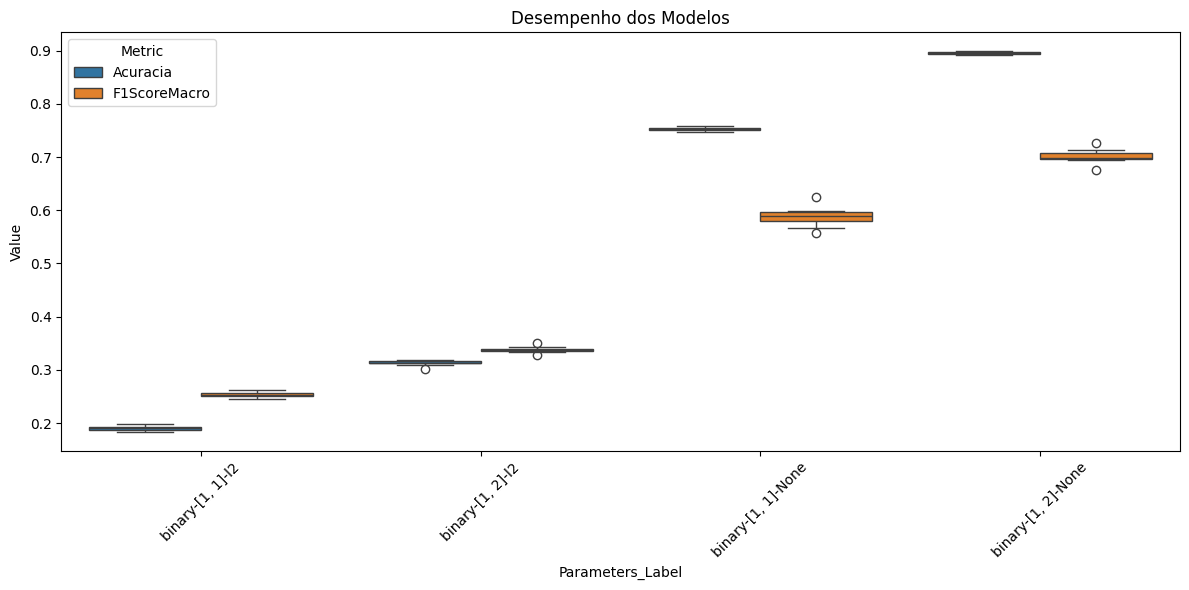
\includegraphics[width=0.8\textwidth]{images/boxbinario.png}
    \caption{Boxplot dos F1 Scores Macro das combinações Argmax para o método Binary.}
    \label{fig:boxplot_binary}
\end{figure}

O gráfico de dispersão, \ref{fig:scatter_acuracia_f1score_binary}, ilustra o impacto significativo dos parâmetros de normalização e range de N-Gramas no desempenho do modelo. Configurações sem normalização L2 tendem a agrupar-se no quadrante de desempenho superior, destacando a influência negativa da normalização L2 na classificação binária para este conjunto de dados.  É observável que ao se aplicar o ngram (1,2), as métricas melhoram, indicando melhoria no método.

\begin{figure}[H]
    \centering
    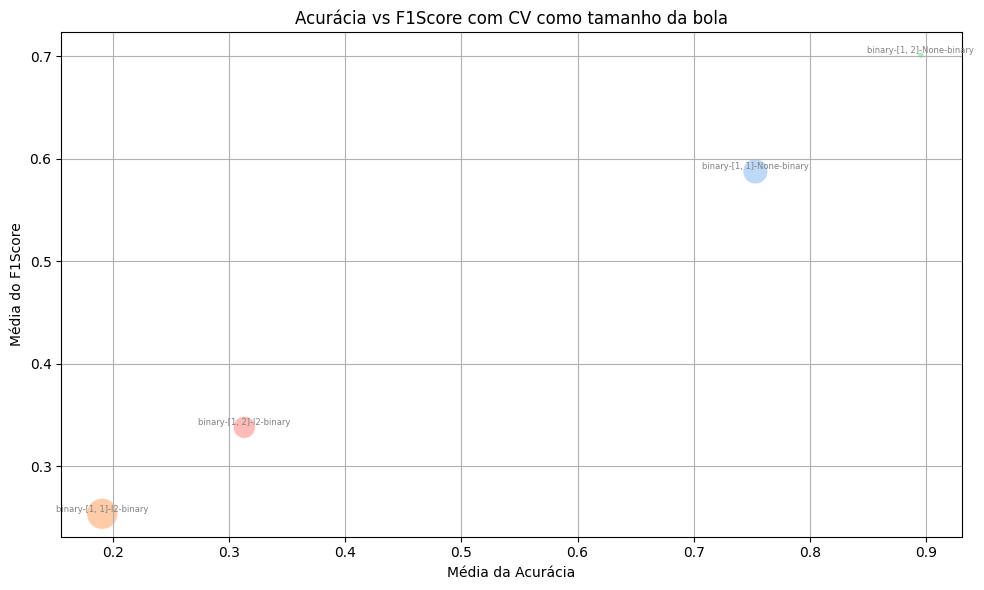
\includegraphics[width=0.8\textwidth]{images/dispersaobinario.png}
    \caption{Gráfico de dispersão relacionando acurácia e F1 Score Macro das combinações Argmax para o método Binary.}
    \label{fig:scatter_acuracia_f1score_binary}
\end{figure}

Em resumo, os resultados sugerem que a ausência de normalização L2, combinada com o uso de bigramas, otimiza significativamente o desempenho da classificação binária. Esse padrão pode ser atribuído à maior capacidade dos bigramas em capturar contextos relevantes sem a penalização da normalização.  É explicável que ao se normalizar um vetor binário, classes com mais termos tendem a possuir valores menores para o token, o que por sua vez perde relevância ao se realizar a avaliação da similaridade.

\subsection{Análise do Método TermFrequency}

A Tabela \ref{tab:resultadoargmaxtf_rankings} apresenta os resultados para o método tf.  Os resultados indicam que a configuração utilizando bigramas (NGram [1,2]) com aplicação de normalização L2 alcançou a melhor performance em ambos os indicadores. Especificamente, a configuração TermFrequency [1, 2] com L2 destacou-se, sugerindo que a inclusão de bigramas e a normalização são benéficas para a análise de textos curtos, ao capturar relações contextuais mais complexas e reduzir a influência de termos frequentes, respectivamente.

\begin{table}[H]
\centering
\caption{Resultados estatísticos dos testes para o método Argmax TF}
\label{tab:resultadoargmaxtf_rankings}
\footnotesize % Diminui a fonte da tabela
\begin{tabular}{lllrrrrrr}
\hline
Método & NGram & Norm & \multicolumn{3}{c}{Acurácia (\%)} & \multicolumn{3}{c}{F1 Score Macro(\%)} \\
& & & Média & CV & \# & Média & CV & \# \\
\hline
TermFrequency & [1, 1] & None & 63.76 & 0.41 & 4 & 23.44 & 2.05 & 4 \\
TermFrequency & [1, 1] & L2 & 77.05 & 0.24 & 2 & 52.31 & 2.46 & 2 \\
TermFrequency & [1, 2] & None & 66.68 & 0.28 & 3 & 27.08 & 1.69 & 3 \\
TermFrequency & [1, 2] & L2 & 79.65 & 0.29 & 1 & 55.56 & 2.61 & 1 \\
\hline
\end{tabular}
\end{table}

Os boxplots, \ref{fig:boxplot_tf}, associados a estas configurações ilustram uma variância reduzida nos resultados de acurácia e F1Score não normalizado.  Quando ocorre normalização a um leve aumenta da dispersão em relação ao F1Score. Novamente, a correlação entre os rankings de acurácia e F1 Score Macro reforça a ideia de que as configurações que performam bem em uma métrica tendem a performar bem na outra, demonstrando uma correlação em performar bem em uma métrica implica em performar bem em outra, medida global e medida interna.

\begin{figure}[H]
    \centering
    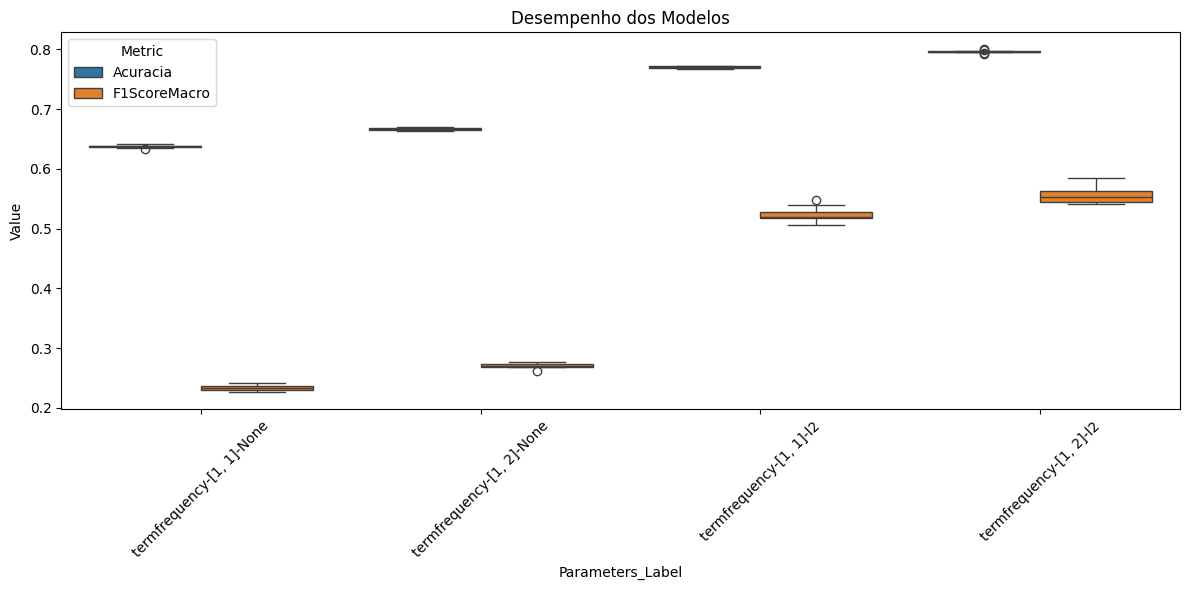
\includegraphics[width=0.8\textwidth]{images/boxtf.png}
    \caption{Boxplot dos F1 Scores Macro das combinações Argmax para o método TFIDF.}
    \label{fig:boxplot_tf}
\end{figure}

O gráfico de dispersão, \ref{fig:scatter_tf}, permite observar o maior ganho, quando aplicado sobre a normalização. 
 Por outro lado aumentar a quantidade de tokens não influencia de maneira significativa a performance do modelo.  A normalização incrementa significativamente a performance sobre a métrica F1Score, devido a tirar o efeito do desbalanceamento.  

\begin{figure}[H]
    \centering
    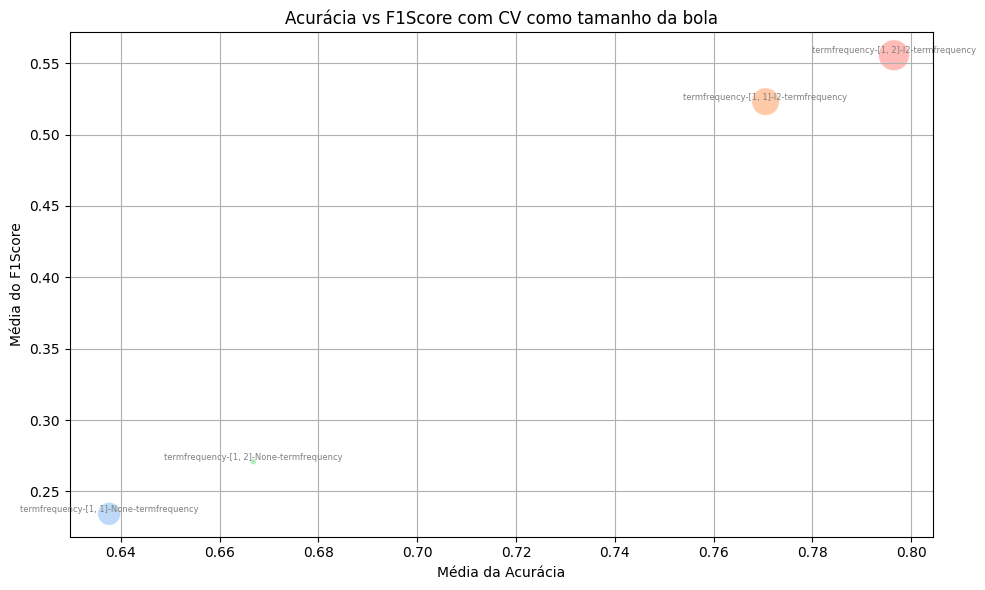
\includegraphics[width=0.8\textwidth]{images/dispersaotf.png}
    \caption{Gráfico de dispersão relacionando acurácia e F1 Score Macro das combinações Argmax para o método TFIDF.}
    \label{fig:scatter_tf}
\end{figure}

Em suma, a análise do método TF revela uma preferência clara pelas configurações que utilizam bigramas em conjunto com normalização L2. Sendo a normalização que apresenta o maior impacto.


\subsection{Análise do Método TFIDF}

A análise dos resultados obtidos pelo método TFIDF, conforme apresentado na Tabela \ref{tab:resultadoargmaxtfidf_rankings}, destaca que configuração TFIDF [1, 2] e L2 como a mais eficaz, alcançando a maior média tanto em acurácia (82.76\%) quanto em F1 Score Macro (59.83\%). Tal configuração sugere que a utilização de bigramas, ao adicionar uma camada de análise contextual, juntamente com a normalização L2, que penaliza termos excessivamente frequentes, cria um equilíbrio ideal para a captura de nuances linguísticas em textos curtos.

O impacto da normalização L2, em particular, merece destaque. Ao comparar as configurações com e sem normalização L2, observa-se uma melhoria consistente nos resultados quando a normalização é aplicada. Isso indica que a redução da influência de termos de alta frequência pode ser crucial para aumentar a eficácia da classificação, especialmente em conjuntos de dados onde a prevalência de certos termos pode distorcer a representação do texto.

\begin{table}[H]
\centering
\caption{Resultados estatísticos dos testes para o método TFIDF com diferentes configurações}
\label{tab:resultadoargmaxtfidf_rankings}
\footnotesize % Diminui a fonte da tabela
\begin{tabular}{lllrrrrrr}
\hline
Método & NGram & Norm & \multicolumn{3}{c}{Acurácia (\%)} & \multicolumn{3}{c}{F1 Score Macro(\%)} \\
& & & Média & CV & \# & Média & CV & \# \\
\hline
TFIDF & [1, 1] & None & 70.64 & 0.28 & 4 & 32.10 & 2.25 & 4 \\
TFIDF & [1, 1] & L2 & 78.37 & 0.32 & 3 & 55.20 & 2.47 & 3 \\
TFIDF & [1, 2] & None & 74.57 & 0.33 & 2 & 37.67 & 1.53 & 2 \\
TFIDF & [1, 2] & L2 & 82.76 & 0.29 & 1 & 59.83 & 2.52 & 1 \\
\hline
\end{tabular}
\end{table}

Os boxplots, \ref{fig:boxplot_tfidf} permite novamente verificar a correlação entre acurácia e f1score.  Além disto, percebe-se o impacto normalização sendo o mais impactante, promovendo tanto ganho em acurácia quando ganho em f1score.  Novamente o F1Score apreenta um ligeiro aumento de variabilidade quando se aplica a normalização, e por fim, o impacto do aumento de termos, ngram (1,2), melhora o desempenho, mas não na mesma intensidade que a normalização..


% Boxplot e Gráfico de Dispersão para o método TFIDF
\begin{figure}[H]
    \centering
    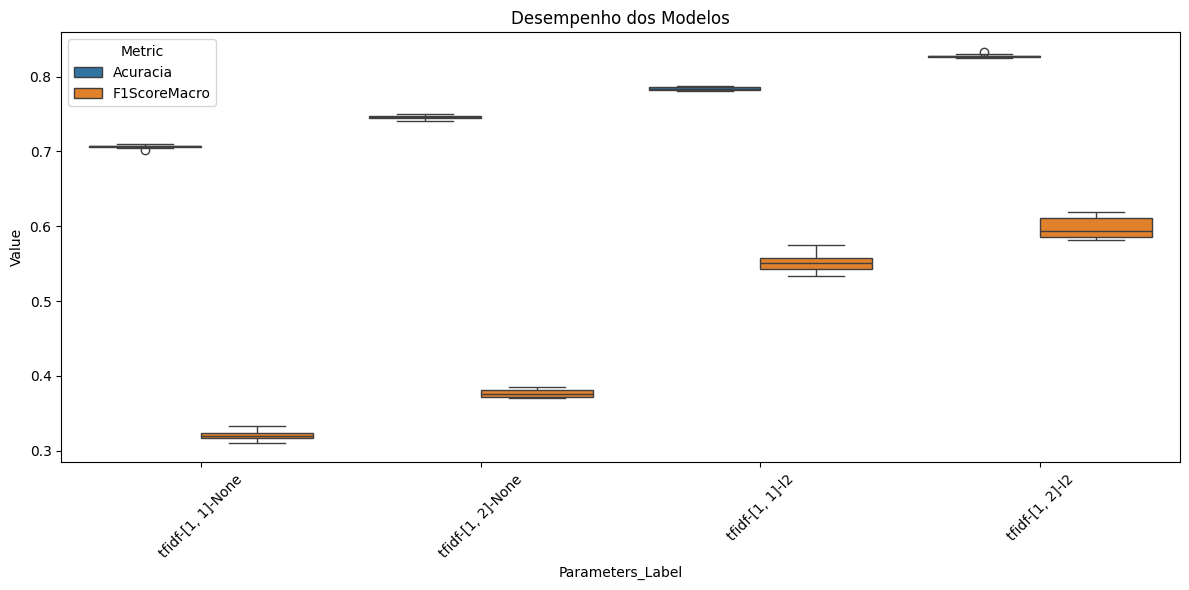
\includegraphics[width=0.8\textwidth]{images/boxtfidf.png}
    \caption{Boxplot dos F1 Scores Macro das combinações Argmax para o método TFIDF.}
    \label{fig:boxplot_tfidf}
\end{figure}

O gráfico de dispersão, \ref{fig:scatter_tfidf}, permite confirmar visualmente a análise acima de maneira combinda.  

\begin{figure}[H]
    \centering
    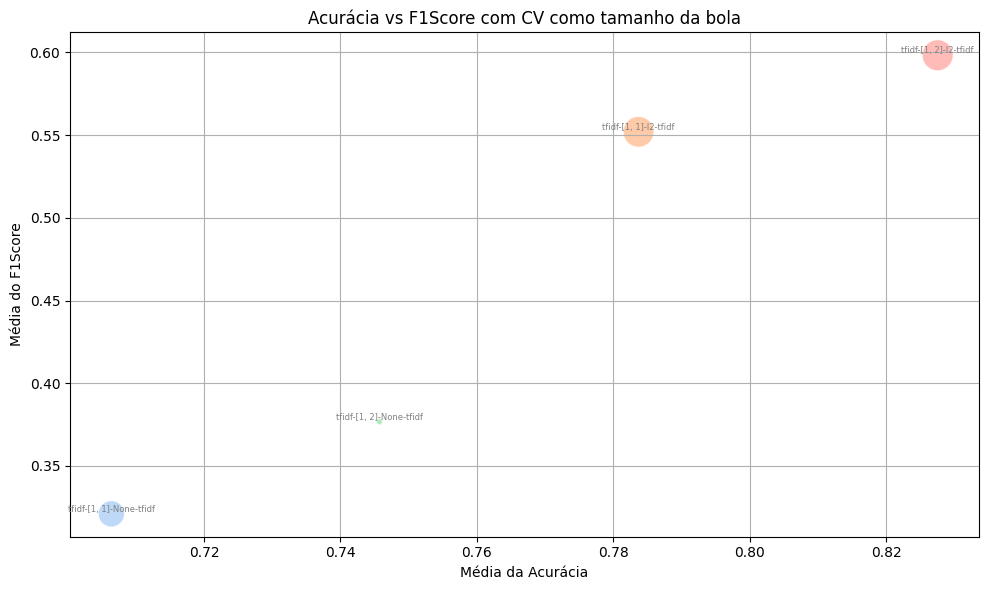
\includegraphics[width=0.8\textwidth]{images/dispersaotfidf.png}
    \caption{Gráfico de dispersão relacionando acurácia e F1 Score Macro das combinações Argmax para o método TFIDF.}
    \label{fig:scatter_tfidf}
\end{figure}

Em conclusão, a normalização L2 provoca a maior alteração nos resultados, seguido de uma melhora não tão significativa dada pela tokenização.


\subsection{Considerações Finais sobre Configurações Testadas}

Ao finalizar a avaliação das diversas configurações testadas para os métodos de classificação Argmax, emerge um panorama claro sobre a influência dos parâmetros de normalização e n-gram na eficácia da classificação de textos curtos. Esta seção visa sintetizar as conclusões extraídas das análises anteriores e discutir as implicações práticas destes achados.

A Tabela \ref{tab:resumo_parametros} apresenta os parâmetros sugeridos para cada modelo bem como o parâmetro que promove o maior impacto.

\begin{table}[H]
\centering
\caption{Parâmetros sugeridos para os métodos Argmax baseados em Acurácia e F1 Score Macro ($^*$ parâmetro mais impactante)}
\label{tab:resumo_parametros}
\begin{tabular}{lcc}
\hline
\textbf{Método} & \textbf{Normalização} & \textbf{N-Gram} \\
\hline
Binary & None$^*$ & [1, 2] \\
TermFrequency & L2$^*$ & [1, 2] \\
TFIDF & L2 & [1, 2]$^*$ \\
\hline
\end{tabular}
\end{table}

Neste segmento, são resumidos os principais achados decorrentes da avaliação das configurações testadas nos métodos de classificação Argmax, com ênfase na influência exercida pelos parâmetros de normalização e n-gram sobre a eficácia da classificação de textos curtos. Os padrões identificados nas preferências de configuração para cada método de classificação são delineados a seguir em forma de pontos-chave:

\begin{itemize}
    \item Para o método Binary:
    \begin{itemize}
        \item A ausência de normalização L2 foi determinante para alcançar melhores resultados, sugerindo que, no contexto binário, a normalização pode penalizar classes com uma diversidade maior de termos.
        \item A utilização de bigramas [1, 2] contribuiu para uma melhoria secundária, evidenciando que a presença ou ausência de termos constitui um fator impactante na classificação.
    \end{itemize}
    \item Para os métodos TermFrequency e TFIDF:
    \begin{itemize}
        \item A aplicação da normalização L2, em combinação com bigramas [1, 2], foi identificada como a configuração mais eficaz, sublinhando a importância da normalização para contrabalançar a influência de termos frequentes e da expansão contextual para enriquecer a representação textual.
        \item A normalização L2 assume um papel primordial no método TermFrequency, enquanto sua relevância é secundária no método TFIDF, o qual intrinsecamente ajusta a influência de termos frequentes através de sua formulação.
        \item A inclusão de bigramas [1, 2] melhorou o desempenho dos modelos, indicando que a captura de contexto adicional beneficia a classificação.
    \end{itemize}
\end{itemize}



\subsubsection{Aplicação das Métricas Propostas e Resultados}

As métricas propostas foram aplicadas ao conjunto de variações dos métodos baseados em argmax, cujos resultados são apresentados na Tabela \ref{tab:Índice de Eficiência Geral (IEG) e Estabilizado (IEGE)}. Observa-se que essas métricas fornecem um índice unificado capaz de refletir eficientemente o desempenho dos métodos tanto em aspectos gerais quanto específicos. Notavelmente, a análise revela uma similaridade nos resultados entre o IEG e o IEGE, o que pode ser atribuído à pouca variação nos coeficientes de variação entre os diferentes métodos avaliados. Essa característica sublinha a possibilidade de classificar os métodos desde a melhor até a pior configuração de maneira consistente, corroborando os resultados observados em diversas representações gráficas neste estudo.

\begin{table}[H]
\centering
\caption{Índice de Eficiência Geral (IEG) e Estabilizado (IEGE)}
\label{tab:Índice de Eficiência Geral (IEG) e Estabilizado (IEGE)}
\footnotesize % Diminui a fonte da tabela
\begin{tabular}{lllrrrrrrrrrr}
\hline
Método & NGram & Norm & \multicolumn{3}{c}{Acurácia (\%)} & \multicolumn{3}{c}{F1 Score Macro (\%)} & \multicolumn{2}{c}{IEG} & \multicolumn{2}{c}{IEGE} \\
& & & Média & CV & \# & Média & CV & \# & Valor & Rank & Valor & Rank \\
\hline
Binary & [1, 2] & None & 89.56 & 0.21 & 1 & 70.09 & 1.91 & 1 & 80.4 & 1 & 79.7 & 1 \\
TFIDF & [1, 2] & L2 & 82.76 & 0.29 & 2 & 59.83 & 2.52 & 2 & 72.2 & 2 & 71.5 & 2 \\
TF & [1, 2] & L2 & 79.65 & 0.29 & 3 & 55.56 & 2.61 & 4 & 68.7 & 3 & 68.0 & 3 \\
TFIDF & [1, 1] & L2 & 78.37 & 0.32 & 5 & 55.20 & 2.47 & 6 & 67.8 & 4 & 67.1 & 4 \\
Binary & [1, 1] & None & 75.31 & 0.44 & 6 & 58.77 & 3.15 & 3 & 67.5 & 5 & 66.6 & 5 \\
TF & [1, 1] & L2 & 77.05 & 0.24 & 4 & 52.31 & 2.46 & 5 & 65.9 & 6 & 65.2 & 6 \\
TFIDF & [1, 2] & None & 74.57 & 0.33 & 7 & 37.67 & 1.53 & 7 & 59.1 & 7 & 58.7 & 7 \\
TFIDF & [1, 1] & None & 70.64 & 0.28 & 8 & 32.10 & 2.25 & 9 & 54.9 & 8 & 54.5 & 8 \\
TF & [1, 2] & None & 66.68 & 0.28 & 9 & 27.08 & 1.69 & 10 & 50.9 & 9 & 50.6 & 9 \\
TF & [1, 1] & None & 63.76 & 0.41 & 10 & 23.44 & 2.05 & 12 & 48.0 & 10 & 47.7 & 10 \\
Binary & [1, 2] & L2 & 31.30 & 1.48 & 11 & 33.82 & 1.77 & 8 & 32.6 & 11 & 32.1 & 11 \\
Binary & [1, 1] & L2 & 19.07 & 2.40 & 12 & 25.39 & 2.04 & 11 & 22.5 & 12 & 22.0 & 12 \\
\hline
\end{tabular}
\end{table}




% % Repita a estrutura acima para cada método de ML analisado
% % Exemplo para um método de ML: SVM
% \section{Análise dos Resultados do Método SVM}
% \subsection{Resultado Geral}
% \subsubsection{Box Plot}
% \subsubsection{Tabela de Desempenho}
% \subsubsection{Análise ANOVA}

% \subsection{Impacto do Método de Vetorização}
% \subsubsection{Box Plot}
% \subsubsection{Tabela de Desempenho}
% \subsubsection{Análise ANOVA}

% \subsection{Impacto da Tokenização}
% \subsubsection{Box Plot}
% \subsubsection{Tabela de Desempenho}
% \subsubsection{Análise ANOVA}

% \subsection{Impacto da Normalização}
% \subsubsection{Box Plot}
% \subsubsection{Tabela de Desempenho}
% \subsubsection{Análise ANOVA}

% \subsection{Discussão dos Resultados do SVM}
% Discussão detalhada dos resultados obtidos com o método SVM, fazendo conexões com estudos anteriores e teorias relevantes.

% % Adicione seções similares para outros métodos de ML aqui

% \section{Resultado Geral Comparativo}
% Esta seção compara os resultados obtidos de todos os métodos analisados, destacando as principais diferenças e semelhanças em termos de desempenho.

% \subsection{Box Plots Comparativos}
% \subsection{Tabelas de Desempenho Comparativas}
% \subsection{Análise ANOVA Geral}

% \section{Considerações sobre os Resultados}
% Discussão sobre as limitações dos resultados, possíveis viéses e sugestões para pesquisas futuras.

% \section{Conclusões da Seção de Resultados}
% Sumário dos achados mais significativos desta seção, reiterando a contribuição dos resultados para os objetivos da pesquisa.




% \chapter{Conclusão}
% \section{Resumo dos Achados}
% \section{Contribuições da Pesquisa}
% \section{Limitações do Estudo}
% \section{Sugestões para Trabalhos Futuros}

\chapter{Conclusão}

Neste estudo, investigou-se a eficácia de algoritmos simples de recuperação da informação, combinados com técnicas de pré-processamento e otimização de parâmetros, na classificação de descrições curtas de produtos em português. A análise fundamentou-se na hipótese de que tais algoritmos, quando devidamente ajustados, poderiam melhorar significativamente métricas de desempenho como precisão, acurácia, recall e F1-score.

\section{Síntese dos Resultados}

Os resultados apresentados no capítulo de resultados demonstraram que a combinação de métodos de vetorização (como TF e TF-IDF), aplicação de N-gramas e normalização L2 teve um impacto considerável no desempenho dos modelos. Em particular, o método Binary com N-Gram [1, 2] e sem normalização destacou-se, alcançando a maior acurácia (89.56\%) e F1 Score Macro (70.09\%). Da mesma forma, o método TFIDF com N-Gram [1, 2] e normalização L2 também apresentou desempenho robusto, confirmando a hipótese de que a combinação de técnicas apropriadas de pré-processamento e otimização de parâmetros pode efetivamente melhorar os resultados.

\section{Conexão com as Hipóteses e Objetivos}

Confirma-se a hipótese central do estudo, que postulava que algoritmos simples de recuperação da informação poderiam melhorar significativamente a precisão, acurácia, recall e F1-score na classificação de descrições curtas de produtos em português, pelos resultados obtidos. A análise detalhada dos métodos Argmax revelou que, ao aplicar técnicas de vetorização e normalização adequadas, foi possível alcançar melhorias substanciais nas métricas de desempenho.

Atenderam-se aos objetivos específicos delineados na introdução:

1. \textbf{Adaptação de métodos de recuperação da informação:} Adaptaram-se métodos como sacola de palavras, TF e TF-IDF para a classificação de descrições curtas de produtos.
   
2. \textbf{Avaliação de desempenho:} Demonstrou-se que algoritmos simples de recuperação da informação, como TF e TF-IDF, combinados com métricas de similaridade, são eficazes na classificação de textos curtos em português.

3. \textbf{Impacto das técnicas de pré-processamento:} Revelou-se que a normalização L2 e a aplicação de N-gramas (particularmente bigramas) têm um impacto significativo na eficácia dos modelos.

4. \textbf{Otimização de parâmetros:} Identificaram-se, através da validação cruzada e outras técnicas de ajuste, os parâmetros mais adequados para maximizar a acurácia e o F1-score macro dos algoritmos avaliados.

5. \textbf{Métrica unificada:} Propôs-se e aplicou-se uma métrica unificada que combina acurácia e F1-score macro, permitindo uma comparação mais integrada e holística dos resultados.

\section{Implicações e Contribuições}

As principais contribuições deste estudo incluem uma análise aprofundada do desempenho de diferentes algoritmos de recuperação da informação na classificação de textos curtos em português e a apresentação de diretrizes sobre as técnicas de pré-processamento mais eficazes. Além disso, a adaptação de uma métrica unificada para avaliação de desempenho mostrou-se valiosa, proporcionando uma ferramenta adicional para futuras pesquisas na área.

\section{Limitações e Trabalhos Futuros}

Apesar dos resultados promissores, este estudo apresenta algumas limitações. A avaliação foi limitada a descrições curtas de produtos, o que pode não refletir a complexidade de outros tipos de textos em português. Além disso, a análise foi restrita a um conjunto específico de técnicas e parâmetros, sugerindo que futuros estudos poderiam explorar uma gama mais ampla de algoritmos e métodos de pré-processamento.

Além disso, a não utilização de algoritmos de machine learning mais avançados é uma limitação significativa. Conforme apontado em um artigo publicado pelo próprio autor, a partir de uma base de desempenho de ~90\%, é possível aumentar significativamente a precisão utilizando técnicas mais sofisticadas de machine learning.

Pesquisas futuras podem expandir o escopo desta investigação, aplicando os métodos avaliados a diferentes tipos de textos e explorando novas técnicas de recuperação da informação e aprendizado de máquina. Também seria valioso considerar a implementação de modelos mais avançados, como redes neurais profundas, e comparar seus desempenhos com os algoritmos mais simples analisados neste estudo.

Em suma, este estudo fornece uma base sólida para o desenvolvimento de sistemas de classificação de texto eficientes e precisos, adaptados às particularidades do idioma português, contribuindo para o avanço do processamento de linguagem natural e das aplicações de recuperação da informação no contexto do e-commerce e além.

% O texto tem como objetivo construir uma referência de acurácia para o conjunto de dados específico que contém descrições de produtos em Português. Os resultados mostram que o uso de algoritmos de classificação de texto para tarefas de classificação de texto curto em descrições de produtos em Português é uma maneira eficiente.


% O pipeline simples de pré-processamento (minúsculas, remoção de ruídos e tokenização unigrama por espaço), um saco de palavras e um algoritmo resultam em um método viável e rápido para classificar descrições de produtos.

% Em comparação com diferentes métodos, o aprendizado de máquina apresenta os melhores valores para acurácia simples sobre métodos de recuperação de informações baseados em termos contados ou ponderados. Confirmando dados da literatura, as regressões logísticas demonstram o melhor desempenho sobre a acurácia e os melhores parâmetros encontrados foram C igual a 100, solver igual a sage, sem peso de classe e sem penalidade. Máquinas de vetores de suporte demonstraram um resultado melhorado sobre algoritmos de recuperação de informações e não superam a regressão logística. A melhor combinação de hiperparâmetros foi C igual a 100, kernel igual a sigmóide e peso de classe igual a balanceado.


% Entre os métodos de recuperação de informações, argmaxtfidf e argmaxtfidf obtêm resultados semelhantes e argmaxtf obtém o pior resultado.


% A validação cruzada com quatro dobras e mil amostras demonstra viabilidade para encontrar o melhor hiperparâmetro. E a validação cruzada com 30 dobras apresenta uma boa estatística e um baixo desvio para determinar, em média, o melhor algoritmo.

% Como sugestão para trabalhos futuros, sugere-se expandir as técnicas de pré-processamento, como adicionar TAGS, limpar e nomear entidades e usar outras técnicas de incorporação de palavras, como tfidf, tfnorm, word2vec, LDA e FastText. Tokenizar usando bigrama ou skip-gram, tratar palavras fora do vocabulário e aplicar técnicas de seleção variável, como Lasso. Aplicar técnicas de redução de dimensionalidade, como PCA. Aplicar outras técnicas de aprendizado de máquina não apresentadas aqui e, finalmente, aplicar técnicas de balanceamento de amostras.



\chapter*{Referências}
% Adicione suas referências bibliográficas aqui.
\bibliography{referencias} % Nome do arquivo sem a extensão .bib
\bibliographystyle{apalike}  % ou outro estilo de sua preferência, como "apa" ou "ieee"
\addcontentsline{toc}{chapter}{Referências Bibliográficas}

\appendix
\chapter{Apêndices}
\section{Código Fonte para Geração das Matrizes Termos Documento}
\label{appendix:codigo-fonte-matrizes}
A seguir, apresentamos o código fonte utilizado para a geração das matrizes de frequência, TF-IDF e TF-IDF normalizado, juntamente com comentários explicativos:

\begin{verbatim}
from sklearn.feature_extraction.text import CountVectorizer, TfidfVectorizer
from sklearn.preprocessing import normalize
import pandas as pd

# Definindo os textos para as classes ARROZ e FEIJÃO
textos_arroz = ["arroz tio joao 1 kg arroz fumacence parb 1kg"]
textos_feijao = ["feijao carioca 1kg azulao feij 1 kg preto caldao"]

# Unindo os textos das duas classes para análise conjunta
textos = textos_arroz + textos_feijao

# Criando o vetorizador para contagem de frequência dos termos
count_vectorizer = CountVectorizer(token_pattern=r"(?u)\b\w+\b")
X_count = count_vectorizer.fit_transform(textos)

# Criando o vetorizador TF-IDF para calcular a frequência ponderada dos termos
tfidf_vectorizer = TfidfVectorizer(token_pattern=r"(?u)\b\w+\b")
X_tfidf = tfidf_vectorizer.fit_transform(textos)

# Normalizando os valores TF-IDF para obter uma distribuição mais uniforme
X_tfidf_norm = normalize(X_tfidf, norm='l1', axis=1)

# Convertendo os resultados para DataFrames para facilitar a visualização
df_count = pd.DataFrame(X_count.toarray(), 
                        columns=count_vectorizer.get_feature_names_out(), 
                        index=['ARROZ', 'FEIJÃO'])
df_tfidf = pd.DataFrame(X_tfidf.toarray(), 
                        columns=tfidf_vectorizer.get_feature_names_out(), 
                        index=['ARROZ', 'FEIJÃO'])
df_tfidf_norm = pd.DataFrame(X_tfidf_norm.toarray(), 
                             columns=tfidf_vectorizer.get_feature_names_out(), 
                             index=['ARROZ', 'FEIJÃO'])

# Definindo os índices multiníveis para as colunas
metodos = ['Frequência', 'TF-IDF', 'TF-IDF Normalizado']
termos = ['ARROZ', 'FEIJÃO']
colunas = pd.MultiIndex.from_product([metodos, termos], names=['Método', 'Termo'])

# Combinando os DataFrames com índices multiníveis
df_final = pd.concat([df_count.T, df_tfidf.T, df_tfidf_norm.T], axis=1)
df_final.columns = colunas

# Exibindo a tabela em formato LaTeX
print(df_final.to_latex())
\end{verbatim}
\end{table}

% \section{Detalhes sobre o Dataset DARU}
% \section{Código Fonte e Configurações dos Experimentos}


\end{document}

